\documentclass[12pt,letterpaper]{article}

\usepackage{amsmath}
\usepackage{fontspec}
\setromanfont[Ligatures=TeX]{TeX Gyre Pagella}
\usepackage{unicode-math}
\setmathfont{TeX Gyre Pagella Math}
\usepackage[title]{appendix}
\usepackage[margin=1.0in]{geometry}
\usepackage[figuresleft]{rotating}
\usepackage[longnamesfirst]{natbib}
\usepackage{dcolumn}
\usepackage{booktabs}
\usepackage{multirow}
\usepackage[flushleft]{threeparttable}
\usepackage{setspace}
\usepackage[justification=centering,skip=2pt]{caption}
\usepackage[font=scriptsize]{subfig}
\usepackage[xetex,colorlinks=true,linkcolor=black,citecolor=black,urlcolor=black]{hyperref}
\usepackage{adjustbox}
\usepackage{xfrac}
\usepackage{placeins}

% For word counting uncomment line below and raggedright below
% http://countwordsfree.com/#
% \usepackage[nolists]{endfloat}


% \bibpunct{(}{)}{;}{a}{}{,}
\newcommand{\mco}[1]{\multicolumn{1}{c}{#1}}
\newcommand{\mct}[1]{\multicolumn{2}{c}{#1}}
\newcommand{\mcth}[1]{\multicolumn{3}{c}{#1}}
\newcommand{\X}{$\times$ }
\newcommand{\hs}{\hspace{15pt}}

% Attempt to squeeze more floats in
\renewcommand\floatpagefraction{.9}
\renewcommand\topfraction{.9}
\renewcommand\bottomfraction{.9}
\renewcommand\textfraction{.1}
\setcounter{totalnumber}{50}
\setcounter{topnumber}{50}
\setcounter{bottomnumber}{50}


%------------------------------------------------------------------------


\title{Birth Spacing and Fertility in the Presence of Son Preference and Sex-Selective Abortions:
India's Experience Over Four Decades%
\protect\thanks{%
I am grateful to Andrew Foster and Darryl Holman for discussions about the method.
I owe thanks to Monica Das Gupta, Shelly Lundberg, Daniel Rees, David Ribar, 
Hendrik Wolff, three anonymous reviewers, and seminar participants at University of 
Copenhagen, University of Michigan, University of Washington, University of Aarhus, the 
Fourth Annual Conference on Population, Reproductive Health, 
and Economic Development, and the Economic Demography Workshop for helpful 
suggestions and comments.
I would also like to thank Nalina Varanasi for research assistance.
Support for development of the method from the University of Washington Royalty 
Research Fund and the Development Research Group of the World Bank is gratefully 
acknowledged.
The views and findings expressed here are those of the author and
should not be attributed to the World Bank or any of its member countries.
Partial support for this research came from a Eunice Kennedy Shriver National
Institute of Child Health and Human Development research infrastructure grant,
5R24HD042828, to the Center for Studies in Demography and Ecology at the
University of Washington.
}
}

\author{Claus C P\"ortner\\
    Department of Economics\\
    Albers School of Business and Economics\\
    Seattle University, P.O. Box 222000\\
    Seattle, WA 98122\\
    \href{mailto:cportner@seattleu.edu}{\texttt{cportner@seattleu.edu}}\\
    \href{mailto:claus@clausportner.com}{\texttt{claus@clausportner.com}}\\
    \href{http://www.clausportner.com}{\texttt{www.clausportner.com}}\\
    \& \\
    Center for Studies in Demography and Ecology \\
    University of Washington\\ \vspace{2cm}
    }

\date{August 2020}


%------------------------------------------------------------------------


\begin{document}
\graphicspath{{../figures/}}
\DeclareGraphicsExtensions{.eps,.jpg,.pdf,.mps,.png}

\setcounter{page}{-1}
\maketitle
\thispagestyle{empty}

% \setcounter{page}{0}


\newpage
\thispagestyle{empty}
\doublespacing

\begin{abstract}

% Demography abstract
\noindent 
% In India, the most substantial lengthening in Hindu women's birth intervals over the past 
% four decades has occurred for the women most likely to use sex-selective abortions. 
% For well-educated women with two girls, the median birth interval before the third child 
% has increased by nearly 15 months---and the 75th percentile interval by 21 months---as the 
% sex ratio has approached 80\% boys. 
% Because of the rapid lengthening in spacing, standard fertility rates have significantly 
% overestimated how fast cohort fertility fell. 
% Despite convergence, cohort fertility is still 10\%--20\% higher than the 
% fertility rate and above replacement level for all but the best-educated urban women. 
% With the lengthening from sex selection, some women show a reversal of the traditional 
% spacing pattern; instead of the shortest birth interval in the absence of sons, they now 
% have the longest. 
% Finally, infant mortality has declined over time for all groups, but the decline was 
% fastest for the less educated. 
% Short birth spacing is still associated with higher mortality, although considerably less 
% so for the best-educated women. 
% There is no evidence that the increasing use of sex selection is associated with higher 
% infant mortality. 
% Neither does it appear that the use of sex selection is declining.


\noindent Over the past four decades, the Hindu women in India most likely to use 
sex-selective abortions---well-educated women with no sons---had the most substantial 
lengthening of birth intervals and the most biased sex ratios. 
As a result, we now see cases that reverse the traditional spacing pattern, with some
women with no sons having longer birth intervals than those with sons. 
Those least likely to use sex-selective abortions---less-educated women in rural 
areas---still follow the traditional pattern of short spacing when they have girls, with 
only limited evidence of sex selection. 
Because of the rapid lengthening in spacing, the standard fertility rates substantially 
overestimated how fast cohort fertility fell. 
Despite a convergence, cohort fertility is still 10\%--20\% higher than the fertility rate 
and above replacement level for all but the best-educated urban women. 
Infant mortality has declined substantially over time for all groups, with the fastest 
decline among the less educated. 
Short birth spacing is still associated with higher mortality, although considerably less 
so for the best-educated women. 
There is no evidence that repeated sex-selective abortions are associated with higher 
infant mortality for the child eventually born. 
Finally, it does not appear that the use of sex selection is declining.




% I show that, in India, the most substantial increases in Hindu women's
% birth interval over the last four decades came from the increasing use
% of sex-selective abortions. The women most likely to use sex
% selection---well-educated with no sons---had the most substantial
% lengthening of birth intervals and the most biased sex ratios. 

\noindent JEL: J1, O12, I1

\noindent Keywords: India, prenatal sex determination, censoring, competing risk, 
nonproportional hazard
\end{abstract}

\newpage


%------------------------------------------------------------------------

\section{Introduction\label{sec:intro}}

% For word counting remove comment on the line below
% \raggedright


% Background
India has experienced many positive changes over the past four decades:
The economy has grown substantially,
educational attainment has increased for males and females,
and the total fertility rate has fallen to 2.2 children
\citep{Bosworth2008,Dharmalingam2014,
International-Institute-for-Population-Sciences-IIPS2017}.

However, India also witnessed the advent of sex selection---the selective abortion of 
female fetuses based on prenatal sex determination---with the introduction of ultrasound 
in the mid-1980s.
Combined with a strong continued preference for sons, the result was a dramatic increase 
in the male--female ratio at birth
\citep{das_gupta97,Arnold2002,retherford03b,Guilmoto2012,Portner2015b,Jayachandran2017}.


% Questions addressed and why valuable
The main question I address here is how birth spacing responded to these changes, 
especially the spread of sex selection. 
The motivation is twofold.
First, researchers have failed to appreciate that each abortion increases the
interval between births by 6--12 months.%
\footnote{
The increase consists of three parts. 
First, after an abortion, the uterus needs at least two menstrual cycles to recover, 
or the likelihood of spontaneous abortion increases substantially \citep{zhou00b}. 
Second, the waiting time to conception is one to six months. 
Finally, sex determination tests are reliable only from three months of gestation. 
}
Hence, the growing use of sex-selective abortions may substantially increase birth spacing, 
although we do not know to what extent. 
Second, greater educational attainment by women, higher household income, and the low and 
declining female labor force participation all likely influence birth spacing. 
Thus, the combined changes in birth spacing may outpace what we have observed in 
other countries.

Studying birth spacing contributes to our understanding of fertility decisions, but, equally 
important, birth spacing also affects the reliability of our fertility measures and may 
affect mortality. 
Therefore, I address two additional questions. 

First, did changes in birth spacing bias the fertility estimates for India? 
With longer spacing, mothers will be older at each parity, and this tempo effect makes the 
total fertility rate a downward-biased estimate of cohort fertility
\citep{Hotz1997,Bongaarts1999,Ni-Bhrolchain2011}. 
Hence, if birth intervals increased substantially, then India's fertility may be higher 
than generally accepted.

Second, what is the relationship between infant mortality and the changes in birth spacing 
and sex selection?
In India, birth intervals have traditionally been shorter with fewer sons, contributing 
to the higher mortality risk for girls
\citep{Whitworth2002,Bhalotra2008,Maitra2008,Jayachandran2011,Jayachandran2017a}.
Therefore, longer birth spacing, whether from sex selection or secular changes, may reduce 
mortality \citep{Conde-Agudelo2012,Molitoris2019}.
However, a counteracting effect is possible if longer birth intervals arise from multiple 
abortions because the short duration between pregnancies could increase mortality. 
% Nevertheless, there has been no attempt to examine how infant mortality has changed with 
% the increase in sex selection.


% How the study progresses
To investigate how birth spacing has changed, I use a competing risk hazard model with 
two exit states: The birth of a girl or the birth of a boy. 
I apply the model to the birth histories of Hindu women covering 1972--2016 using 
data from the four National Family and Health Surveys (NFHS). 

The primary outcomes I examine are the 25th, 50th, and 75th percentile birth intervals;
the sex ratio at birth; and the likelihood of giving birth. 
I estimate the model across four periods to capture the changing access and 
legality of sex selection. 
The key variables are maternal education, the sex of previous children, and the area of 
residence.

The empirical model allows me to predict cohort fertility. 
To examine whether tempo effects bias our standard fertility measures, I compare 
the predicted cohort fertility with fertility calculated from age-specific fertility 
rates.

I use the same data to study how infant mortality changed with birth spacing and 
the increasing use of sex selection. 
The key explanatory variables remain the same, except for the addition of birth spacing 
and the sex of the index child. 

% Main results
There are three main results.

First, birth intervals lengthened over the four decades, and the lengthening was longer, 
the higher the parity, the more educated the woman, and the higher the percentile. 
Women most likely to use sex selection---well-educated women with no sons---had the most 
substantial lengthening of birth intervals and the most biased sex ratios. 
As a result, we now see cases that reverse the traditional spacing pattern, with some 
women with no sons having \emph{longer} birth intervals than those with sons. 
Those least likely to use sex selection---less-educated women in rural areas---still follow the 
traditional pattern of short spacing when they have girls, with only some evidence of sex 
selection. 
The likelihood of a very short birth interval changed little. 

Second, the fertility rate substantially overestimated how fast cohort fertility fell in the 
1990s and early 2000s as spacing began to increase. 
Although the two have lately been converging, the predicted cohort fertility is still 
10\%--20\% higher than the fertility rate. 
Furthermore, predicted cohort fertility is still at or above replacement level for all but 
the best-educated urban women. 

Finally, infant mortality has declined substantially over time for all groups, but fastest 
for the less educated, who are now close to the level of the best-educated women. 
However, mortality is still inversely related to education level, especially for very short 
birth intervals. 
There is no evidence that repeated sex-selective abortions are associated with higher 
mortality for the child eventually born.

%------------------------------------------------------------------------------------

% Combine descriptive and theory sections into one

\section{Background and Conceptual Framework}

To set the stage for the subsequent analyses and provide a conceptual framework for 
understanding birth spacing, I first discuss female education and labor force 
participation in India and relevant theories on birth spacing.

% [Female education]

Female education is a crucial explanatory variable here for three reasons.
First, higher female education is associated with lower fertility and increased use of 
sex selection
\citep{das_gupta97,dreze01,bhat03,retherford03b,Guilmoto2009a,Portner2015b,Jayachandran2017}.
Second, female labor force participation in India, as in other developing countries, 
first decreases and then increases with education
\citep{Klasen2015,Fletcher2017,Afridi2018,Bhargava2018,Chatterjee2018,Bhargava2019}.
Finally, child mortality decreases with maternal education
\citep{Rosenzweig1982a,Whitworth2002,Maitra2008}.

% [TK where to put son preference discussion?]
% %
% \footnote{
% It is also possible that the effect is driven by a stronger son preference, although 
% higher education women have shown declining son preference \citep{bhat03,pande07}.
% }

I divide education levels into four groups: No education, 1--7 years, 8--11 years, and 
12 and more years.
The latter two correspond to having completed primary and secondary school, 
respectively.%
\footnote{
Although there are variations by state, elementary education in India consists of a 
primary school covering grades one through five and an upper primary---or middle 
school---covering grades six through eight. 
Similarly, secondary education covers grades nine and tenth for ``secondary education'' 
and 11 and 12 for ``upper secondary.''
}
To ensure that the results are comparable with the prior literature on fertility
and mortality in India, I follow the NFHS reports, except that I combine the 
less than five years and 5--7 years of schooling completed and the 8--9 
and 10--11 years of schooling completed.
This grouping allows me to capture the differences across education levels discussed below, 
while also having groups large enough for the empirical method.


% [what has happened to education]
Female education has increased substantially over time in rural and urban areas but 
is still substantially higher in urban than in rural areas.
Figure \ref{fig:education_over_time} shows the distribution of schooling by birth 
cohort for urban and rural women, 
20 years or older, whether married or not, based on the four rounds of the NFHS.
In rural areas, women with no education have gone from 90\% for the 1930s cohorts to 
less than 20\% for the 1990s cohorts.
Women with eight or more years of education have gone from almost zero for the 1930 cohort 
to more than 60\% for the 1990s cohorts, with about half in the 8--11 group and the 
other half in the 12 plus group.
In urban areas, the proportions with no education or 1--7 years have each declined 
to just below 10\%.
Most of the increase in urban female education came from the 12 plus group, which 
now accounts for more than half of all urban women for the most recent cohorts.

\begin{figure}[htpb]
\centering
\subfloat[Rural]{
    \begin{minipage}{0.49\textwidth}
        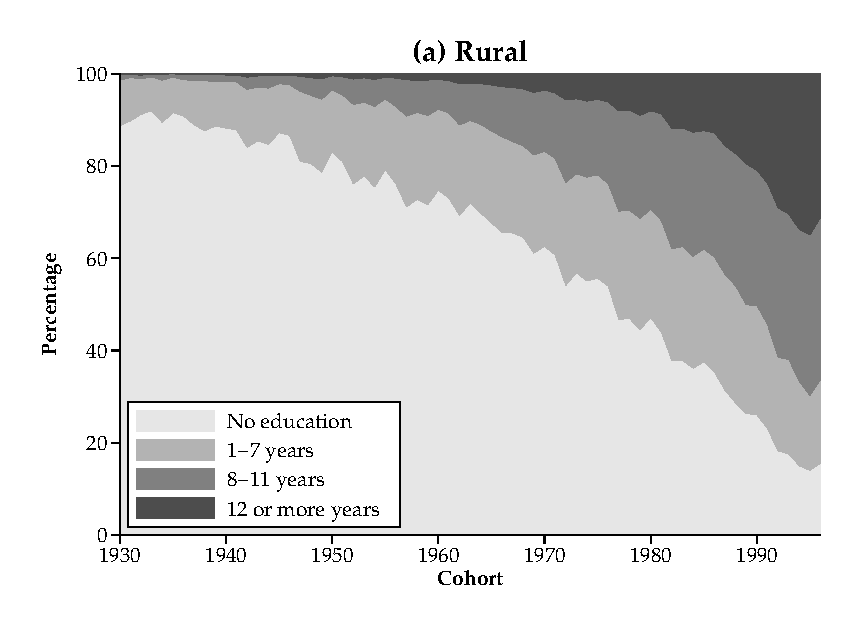
\includegraphics[width=\textwidth]{educ_over_time_rural}
    \end{minipage}
} 
\subfloat[Urban]{
    \begin{minipage}{0.49\textwidth}
        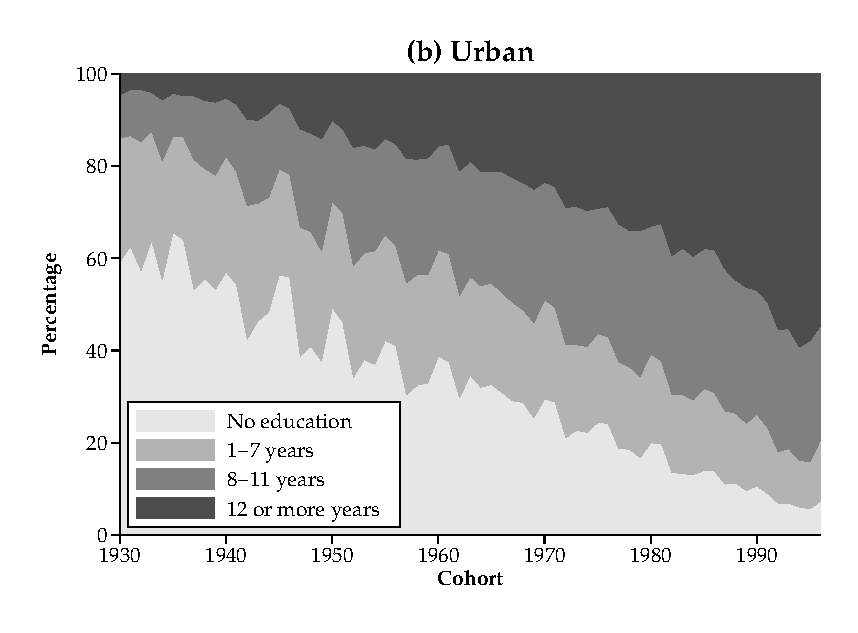
\includegraphics[width=\textwidth]{educ_over_time_urban} 
    \end{minipage}
}
\caption{Distribution of education by cohort for women 20 years or older at survey}
\label{fig:education_over_time}
\end{figure}


% [female labor force participation]

The standard economic argument for shorter spacing with increasing female education 
is that parents incur time costs when they have children \citep{Hotz1997,schultz97}.
Suppose having children requires the mother to reduce her market work. 
Parents can then lower this cost of children by shortening birth spacing to take advantage 
of economies of scale in childrearing  \citep{Vijverberg1982}.

However, even as the level of female education has increased, the female labor force 
participation in both urban and rural areas has stagnated or decreased
\citep{Klasen2015,Fletcher2017,Afridi2018,Bhargava2018,Chatterjee2018,Bhargava2019}.
India's female labor force participation is now lower than that of most other countries and does 
not yet show any signs of increasing \citep{Klasen2015,Chatterjee2018}.
In line with previous research, the NFHS data show a U-shaped relationship between 
education and working for married women, with the highest percentage working being women with 
either no education or 12 or more years and the lowest being women with 8--11 years of education.%
\footnote{
See appendix Figures \ref{fig:work_by_survey} through \ref{fig:work_family_by_survey}. 
}

The low and declining female labor force participation, especially for younger women, 
suggests that families face little incentive to space children more closely 
together for economic reasons.
One explanation is that household income has increased so substantially that the income 
effect dominates any substitution effect.
Two findings speak to this effect.
First, although real wages for both men and women have almost doubled between 1987 and 
2011, the mean male wage is still close to 70\% higher than the female wage 
\citep{Klasen2015,Bhargava2018}.
Second, women’s labor supply appears to be more negatively elastic to husbands' 
wages than positively elastic to their own wages \citep{Bhargava2018}.


% [sex selection]

The introduction of sex selection allows parents to avoid giving birth to girls but 
increases the expected interval to the next birth.
Theory suggests that sex selection increases with lower desired fertility and with
higher parity for a given desired number of children \citep{Portner2015b}.
Sex selection is more widespread among better-educated than less-educated and among urban 
than rural women, which is consistent with lower desired fertility increasing the
use of sex selection 
\citep{das_gupta97,retherford03b,Guilmoto2009a,Portner2015b,Jayachandran2017}.
Better-educated and urban women also tend to live in households with higher income, which 
lowers the relative costs of using sex selection and having long birth intervals.

The combination of rising incomes and continued son preference may lead to even longer 
spacing than might be expected from the income effect alone.
As women's education increases, their productivity in the production of offspring human 
capital also increases.
With relatively more boys born because of increased access to sex-selective 
abortions and the increasing income potential for (male) offspring, demand for 
better-educated women can increase, even if they do not participate in the labor market 
\citep{Behrman1999}.

If more and ``better'' parental attention per child results in higher child ``quality,'' 
we should expect longer birth intervals \citep{Zajonc1975,Zajonc1976,Razin1980}.
However, the evidence on spacing's effect on child quality measures such as IQ 
and education is mixed for developed countries and nonexisting for developing countries
\citep{Powell1993,Pettersson-Lidbom2009,Buckles2012,Barclay2017}.
The exception is health and mortality, where longer spacing does lead to better outcomes, 
although this relationship weakens with maternal education 
\citep{Whitworth2002,Conde-Agudelo2012,Molitoris2019}.

% If parents realize that longer spacing leads to better child outcomes, we may even observe 
% later conception, especially when, with sex selection, the next child is likely to be a boy.
% Working in the opposite direction of this "delay" effect is that women with more education 
% can, in principle, space their children closer together without substantially increasing 
% child mortality risk. 
% However, given the apparent lack of pressure to return to the labor force, this effect is 
% likely small.

% Sanskritization

The increases in female educational attainment imply that access to education has 
expanded beyond the higher castes. 
One possible effect of the associated change in the composition of better-educated women 
is that this group's behavior would change.
However, ``Sanskritization'' implies that as lower-castes females gain access to 
education and their husbands' income increases, they adopt higher-caste 
norms such as stronger son preference and a retraction from the formal labor 
market \citep{Srinivas1956,Chen1995,Abraham2013,Chatterjee2018}.
The low and declining female labor force participation suggests that this process still operates.

% Summary / hypotheses

In summary, with substantial increases in husbands' income and a declining female labor 
force participation, I expect a push toward longer birth spacing over time, independent
of education levels, based on the income effects and the effects of spacing
on child outcomes.
Furthermore, I expect birth spacing to increase the most among the better educated 
because their household income increases the most---even with declining female labor 
participation---and because of their use of sex selection.
Even with the substantial increase in the number of better-educated women, 
"Sanskritization" implies that the changing composition will not substantially change 
the use of sex selection.


%------------------------------------------------------------------------------------

\section{Estimation Strategy\label{sec:strategy}}

% Requirements for method and the intuition behind each:  
%  - Account for censoring (hazard model)
%  - Work both with and without sex selection (competing risk part)
%  - Allow for changes in use of sex selection within spell (flexible specification of baseline hazard ?)
%  - Capture that the shape of the hazard function differ across groups
%    (nonproportionality); needs a better description, maybe using example
%    of shorter spacing and/or use of sex selection. Differences in parity
%    progression likelihood. 

The standard approach in the birth spacing literature is to use proportional hazard
models with a single exit---the birth of a child.%
\footnote{
See \citet{Sheps1970} and \citet{Newman1984} for early discussions of why 
hazard models are the preferred way to deal with the censoring of birth
intervals.
}
There are two problems with the standard approach in this setting.

First and foremost, the use of sex selection means that the sex of the next child is 
no longer random and that the spacing to the birth of a boy will differ from the 
spacing to a girl. 
Therefore, I use a competing risk setup that captures both the non-randomness of 
the birth outcome and the differential spacing.%
\footnote{
\cite{Merli2000} used a discrete hazard model to examine whether 
there was underreporting of births in rural China, although they 
estimated separate waiting time regressions for boys and girls.
}

Second, even without sex selection, it is unlikely that characteristics, such as 
the sex composition of previous births, have the same effects throughout the entire 
birth interval. 
The proportional hazard model requires that the hazard for any individual is a 
fixed proportion of the hazard for any other individual. 
Nonconstant effects violate that assumption, and the results from a proportional hazard 
model would, therefore, be biased. 
The proportionality assumption is especially problematic for higher-order birth 
intervals because there are substantial differences across groups in the likelihood 
of progressing to the next birth and how soon couples want their next child if they 
are going to have one \citep{Whitworth2002,Bhalotra2008,Kim2010}.

The introduction of prenatal sex determination exacerbates any bias from
the proportionality assumption for two reasons. 
First, different groups have different levels of sex-selective abortion use and, thereby, 
birth spacing. 
Second, within a birth interval, a household's use of sex selection may vary, and that
means that the effects of covariates vary as well.

Therefore, I use a nonproportional hazard specification that allows the shape of the 
hazard functions to vary across groups.
The use of a nonproportional specification also mitigates any potential effects 
of unobserved heterogeneity when used in conjunction with a flexible baseline hazard 
\citep{Dolton1995}.

The model is a discrete-time, nonproportional, competing risk hazard model with two 
exit states: Either a boy or a girl is born. 
The unit of analysis is a spell---the period from one parity birth to the following 
birth or censoring. 
For estimation purposes, the spells begin nine months after the previous birth because 
this is the earliest we should expect to observe a new birth. 
Censoring can happen for three reasons: The survey takes place, sterilization of the 
woman or her husband, or imposed because of too few births for the method to work.

For each woman, $i=1,\ldots,n$, the starting point for a spell is time $t=1$, and 
the spell continues until time $t_i$, when either birth or censoring of the spell 
occurs.
The time of censoring is assumed to be independent of the hazard rate,
as is standard in the literature.
The two exit states are the birth of a boy, $j=1$, or a girl, $j=2$.

The discrete-time hazard rate $h_{ijt}$ is 
\begin{equation}
 h_{ijt} = \frac{\exp(D_j(t) + \alpha_{jt}'\mathbf{Z}_{it} + \beta_j'\mathbf{X}_{i})} 
 {1 + \sum_{l=1}^2 \exp(D_j(t) + \alpha_{lt}'\mathbf{Z}_{it} + \beta_l'\mathbf{X}_{i})} \: \: \; \; \;  j = 1,2.
 \label{eq:hazard}
\end{equation}
$D_{j}(t)$ is the piece-wise constant baseline hazard for outcome $j$, captured
by dummies and the associated coefficients,
\begin{equation}
D_j(t) = \gamma_{j1} D_1 + \gamma_{j2} D_2 + \ldots + \gamma_{jT} D_T,
\end{equation}
with $D_m = 1$ if $t=m$ and zero otherwise.
This approach to modeling the baseline hazard is flexible and does not restrict the 
baseline hazard unnecessarily.
$\mathbf{Z}$ is the nonproportional part, which includes the interactions between 
$D_j(t)$ and a set of explanatory variables and the interactions of those.
The remaining explanatory variables, $\mathbf{X}$, enter proportionally.


% To further minimize any potential bias from assuming proportionality, estimations 
% are done separately for different levels of mothers' education and different periods.
% I discuss the choice of which variables to use for nonproportionality below.


Equation \ref{eq:hazard} is equivalent to the logistic hazard model and has the same 
likelihood function as the multinomial logit model \citep{allison82,jenkins95}.
Hence, splitting spells into smaller intervals---here equal to three months---and 
treating them as observations, I can estimate the model using a standard multinomial 
logit model. 
% In the reorganized data, the outcome variable is 0 if the woman does not have a child 
% in a given interval (the base outcome), 1 if she gives birth to a son in that interval, 
% and 2 if she gives birth to a daughter in that interval.

I use the model to predict birth interval measures, parity progression probabilities, 
and the sex ratio rather than present coefficients because the interpretation 
of competing risk model coefficients is challenging \citep{thomas96}.
The predicted parity progression probability is the likelihood of giving birth by the
imposed censoring based on standard survival curve calculations averaged across all
women in a given sample.

For birth intervals, I estimate a set of percentile birth intervals. 
I first calculate for each woman when there is a given percentage chance that she will have 
given birth, conditional on the probability of giving birth in the spell. 
For example, with an 80\% parity progression probability, the median birth interval 
is the predicted number of months before a woman passes the 60\% mark on her survival 
curve. 
I then add nine months to account for the start of the spell. 
The reported statistic is the average of a given percentile interval across all women in 
a given sample using the individual progression probabilities as weights.

% The predicted sex ratio is the weighted average of individual predicted sex ratios, using 
% parity progression probabilities as weights.
% For an individual woman, the estimated percent of births that are boys at $t$, $\hat{Y_t}$, is:  
% \begin{equation}
% \hat{Y}_t 
% = 
% \frac{ P(b_{t} | \mathbf{X}_{k}, \mathbf{Z}_{kt},t )}
% { P(b_{t} | \mathbf{X}_{k}, \mathbf{Z}_{kt},t) + P(g_{t} | \mathbf{X}_{k}, \mathbf{Z}_{kt},t )} 
% \times 100,
% \label{eq:probability_son}
% \end{equation}
% where $b$ and $g$ are the predicted probabilities of having a boy and a girl, respectively,
% conditional on the explanatory variables and not having had a child before $t$.
% Weighting the percentages boys with the likelihood of exiting the spell with a birth across all 
% $t$ gives the predicted percent of boys over the entire spell for an individual.%
% \footnote{
% Imagine $T=2$. 
% If 54 and 66 percent of births are boys and the likelihood of giving birth 20 and 40 percent, 
% then the predicted sex ratio is $\frac{54*0.2+66*0.4}{0.2+0.4} = 62$ percent boys. 
% }


The predicted sex ratio is the weighted average of individual predicted sex ratios, using 
parity progression probabilities as weights.
To find the individual sex ratio, I estimate the percentage of births that are boys at $t$, 
conditional on not having had a child before $t$.
Weighting the percent boys with the likelihood of exiting the spell with a birth across all 
$t$ gives the predicted percentage of boys over the entire spell for an individual.%
\footnote{
Imagine $T=2$. 
If 54\% and 66\% of births are boys and the likelihood of giving birth 20\% and 40\%, 
then the predicted sex ratio is $\frac{54*0.2+66*0.4}{0.2+0.4} = 62$\% boys. 
}



\section{Data\label{sec:data}}

The data come from the four rounds of the NFHS
collected in 1992--1993, 1998--1999, 2005--2006, and 2015--2016.
The surveys are large: 89,777, 90,303, 124,385, and 699,686 women, respectively. 
NFHS-1 and NFHS-2 surveyed only ever-married women, while the two later surveys included 
never-married.

I focus on the three spells starting from the first birth and ending with the 
fourth birth.
I exclude the interval from marriage to the first birth because many are imputed and the
higher-order intervals because few women had five or more births, especially among the 
better-educated.

I restrict the sample to Hindus for two reasons.
First, Hindus are the majority population group, about 80\% of India’s population.
Second, the prior literature shows that son preference and use of sex selection vary 
substantially between Hindus and the second largest group, Muslims. 
Combining them and assuming that the baseline hazard is the same would lead to biased 
results.
Because of space constraints and the relatively small number of observations once split 
by education and periods, I do not provide separate results for Muslims or any of the 
remaining groups, such as Sikhs, Jains, and Christians.

Finally, I exclude visitors and women in any of the following categories: Never married; 
no gauna yet; married more than once; divorced; not living with husband; inconsistent age 
at marriage; or education information missing.  
The same goes for women who had at least one multiple births, reported giving birth 
before age 12, had a birth before marriage, or had an interval between births of less than 
nine months. 

In addition to a large number of women surveyed and the long period covered, a significant 
benefit of the NFHS over other surveys is that enumerators pay careful attention to the 
spacing between births and probe for ``missed'' births.
For India, the main concern is underreporting of deceased children, especially a systematic 
recall error where respondents' likelihood of reporting the birth of a deceased child depends 
on the sex of that child.
Unreported deceased children inflate the birth intervals and, with declining mortality, 
make changes over time appear too small.
In the online appendix, I provide a detailed analysis of systematic recall error, which 
shows that recall error depends heavily on how long ago a woman was married. 
I, consequently, drop women married 22 years or more.%
\footnote{
Recall error is likely behind the designation of the first two rounds of NFHS as ``moderate 
quality'' in an analysis of the quality of birth histories in DHS surveys and its impact 
on fertility estimates \citep{Schoumaker2014}.
}

To ensure that there are enough births for the method to work, I censor spells at 96 
months (eight years) after a woman can first give birth, equivalent to 105 months 
after the birth of the prior child.
Less than 1\% of observed births occur after the cutoff.
The final sample consists of 
  395,695 women, with   815,360 parity one through four births.
% [number] women, with [number] parity one through four births.

% %
% \footnote{
% \input{../tables/num_missed.tex}
% }

Direct information on the use of sex selection is not available, so I compare periods 
based on the changes in access and legality of prenatal sex determination in India.
Abortion has been legal in India since 1971.
Reports of sex determination appeared around 1982--1983, and the number of clinics 
quickly increased \citep{Sudha1999,bhat06,Grover2006}.
In 1994, the Prenatal Diagnostic Techniques Act made determining and communicating 
the sex of a fetus illegal.%
\footnote{
% Details about the act are at \href{http://pndt.gov.in/}{http://pndt.gov.in/}.
There is little evidence that the ban significantly affected sex ratios \citep{Das-Gupta2019}.
}
Finally, although sex selection increased even after 1994, we may have passed a 
turning point in its use in the mid-2000s \citep{Das_Gupta2009,Kumar2012,Bongaarts2013,Diamond-Smith2015}.

I use four periods: 1972--1984, 1985--1994, 1995--2004, and 2005--2016.
The first covers the period before sex selection became available and the second from when sex 
selection became available until the Prenatal Diagnostic Techniques Act.
I have split the period from 1995 until 2016 into two to examine if there was support for 
the prior literature's hypothesized reversal in child sex ratios and son 
preference in India.

The allocation of spells into periods is determined by when conception, and, therefore, 
decisions on sex selection can begin. 
Hence, some spells cover two periods, which may bias downward the differences between the 
periods.
Most sterilizations take place soon after giving birth. 
These spells, therefore, do not show up in the samples used. 
Furthermore, sterilization depends strongly on the sex composition of prior children
with lower probabilities, the fewer boys. 
The effect is to bias downward the differences in parity progression probabilities.

I divide the explanatory variables into two groups, nonproportional and proportional. 
The first group consists of characteristics shown in the prior literature to affect the 
spacing choice and the use of sex selection: Mother’s education, sex composition of 
previous children, and area of residence. 
To minimize any potential bias from including proportional variables, I estimate a 
separate model for each birth interval, education group, and period combination, rather 
than including education as a variable. 
I capture sex composition with dummy variables for the possible combinations, ignoring 
the ordering of births.%
\footnote{
With sex selection, the composition of prior children is, in principle, endogenous. 
It is beyond the scope of this paper to develop a method for dealing with this issue. 
}
Area of residence is a dummy variable for living in an urban area.

The second group of variables consists of those expected to have an approximately 
proportional effect on the hazard.
These include the mother's age when the spell begins, the household's
land ownership, and whether it belongs to a scheduled tribe or caste.
Appendix Tables \ref{tab:des_stat1} and \ref{tab:des_stat2} present descriptive statistics.


\section{How Birth Spacing Changed\label{sec:results}}

% Explain question and what I am doing
The first question I address is how birth spacing responded to the significant 
changes in India.
Figures \ref{fig:spacing_low_rural} through \ref{fig:spacing_highest_urban}
show the 25th, 50th, and 75th percentile birth intervals in 
months, the sex ratio, and the probability of having a birth for each spell
by education levels and area of residence.%
\footnote{
Results for urban women without education, rural women with 12 or more years of 
education, and the fourth spell for women with 12 or more years of education are
in the online appendix because of relatively small samples.
}
The sex ratio graphs also show the natural sex ratio, approximately 51.2\% boys
\citep{ben-porath76b,jacobsen99,Portner2015b}.
The underlying values with bootstrapped standard errors are available in the online 
appendix.


\captionsetup[figure]{skip = -16pt}

\begin{figure}
\centering
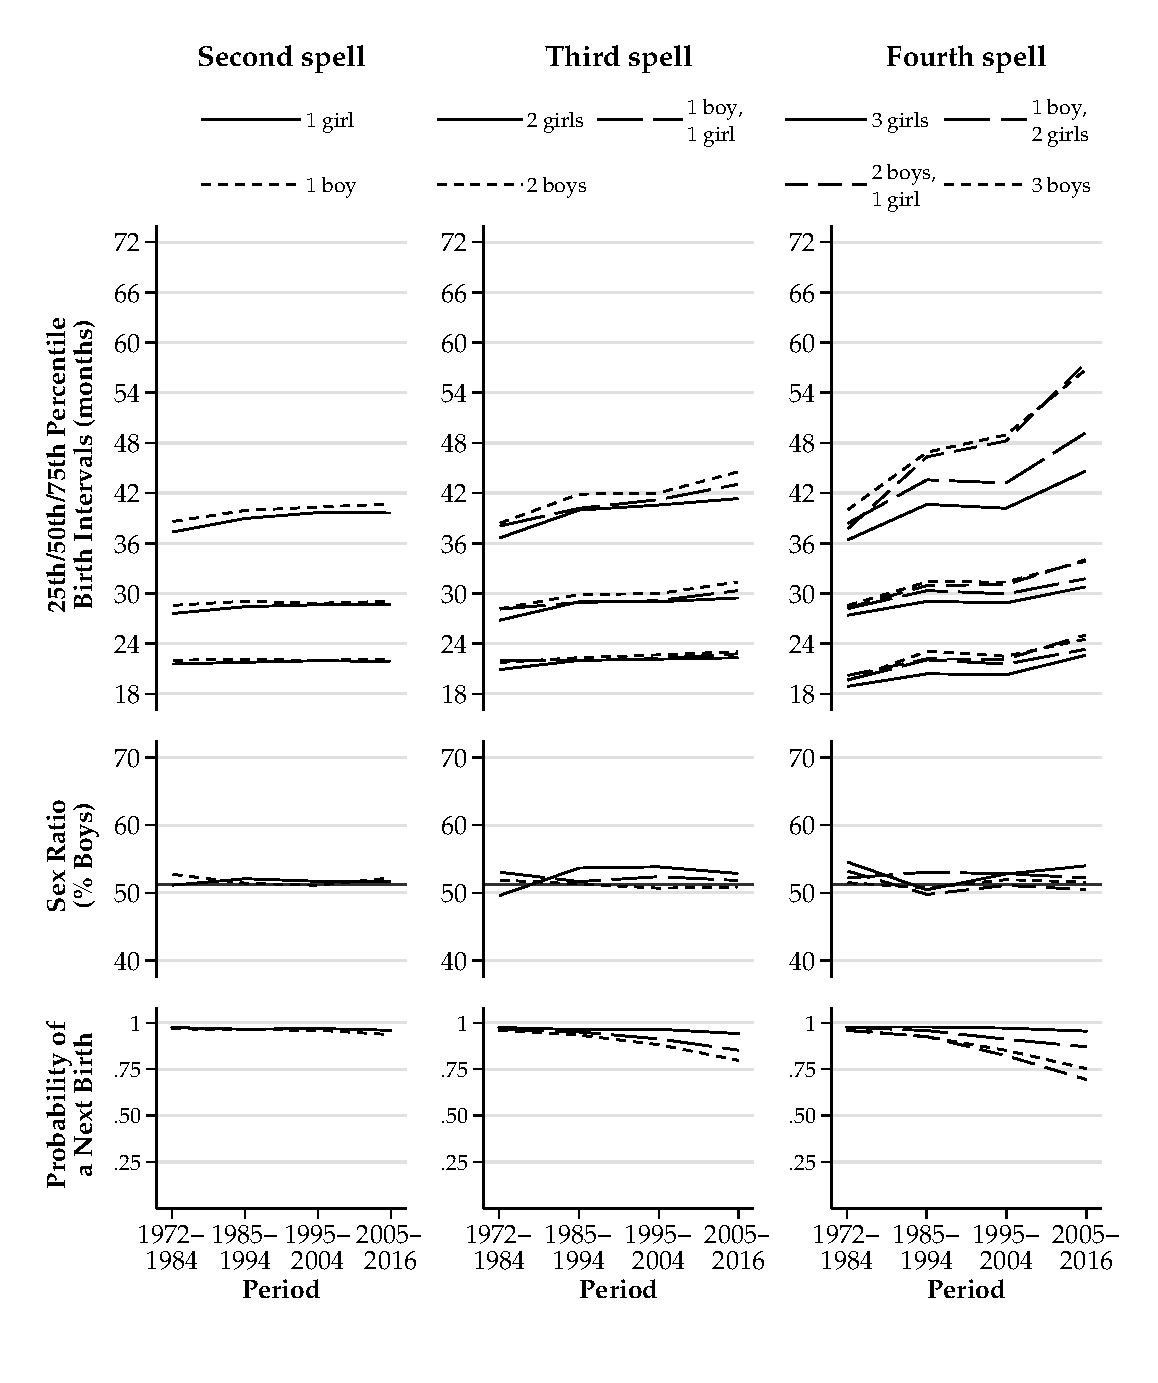
\includegraphics[width=\textwidth,height=\textheight,keepaspectratio=true]{bs_low_rural}
\caption{Percentile birth intervals, sex ratios, and parity progression  
for rural women with no education by spell, sex composition, and period}
\label{fig:spacing_low_rural}
\end{figure}

% \begin{figure}
% \centering
% 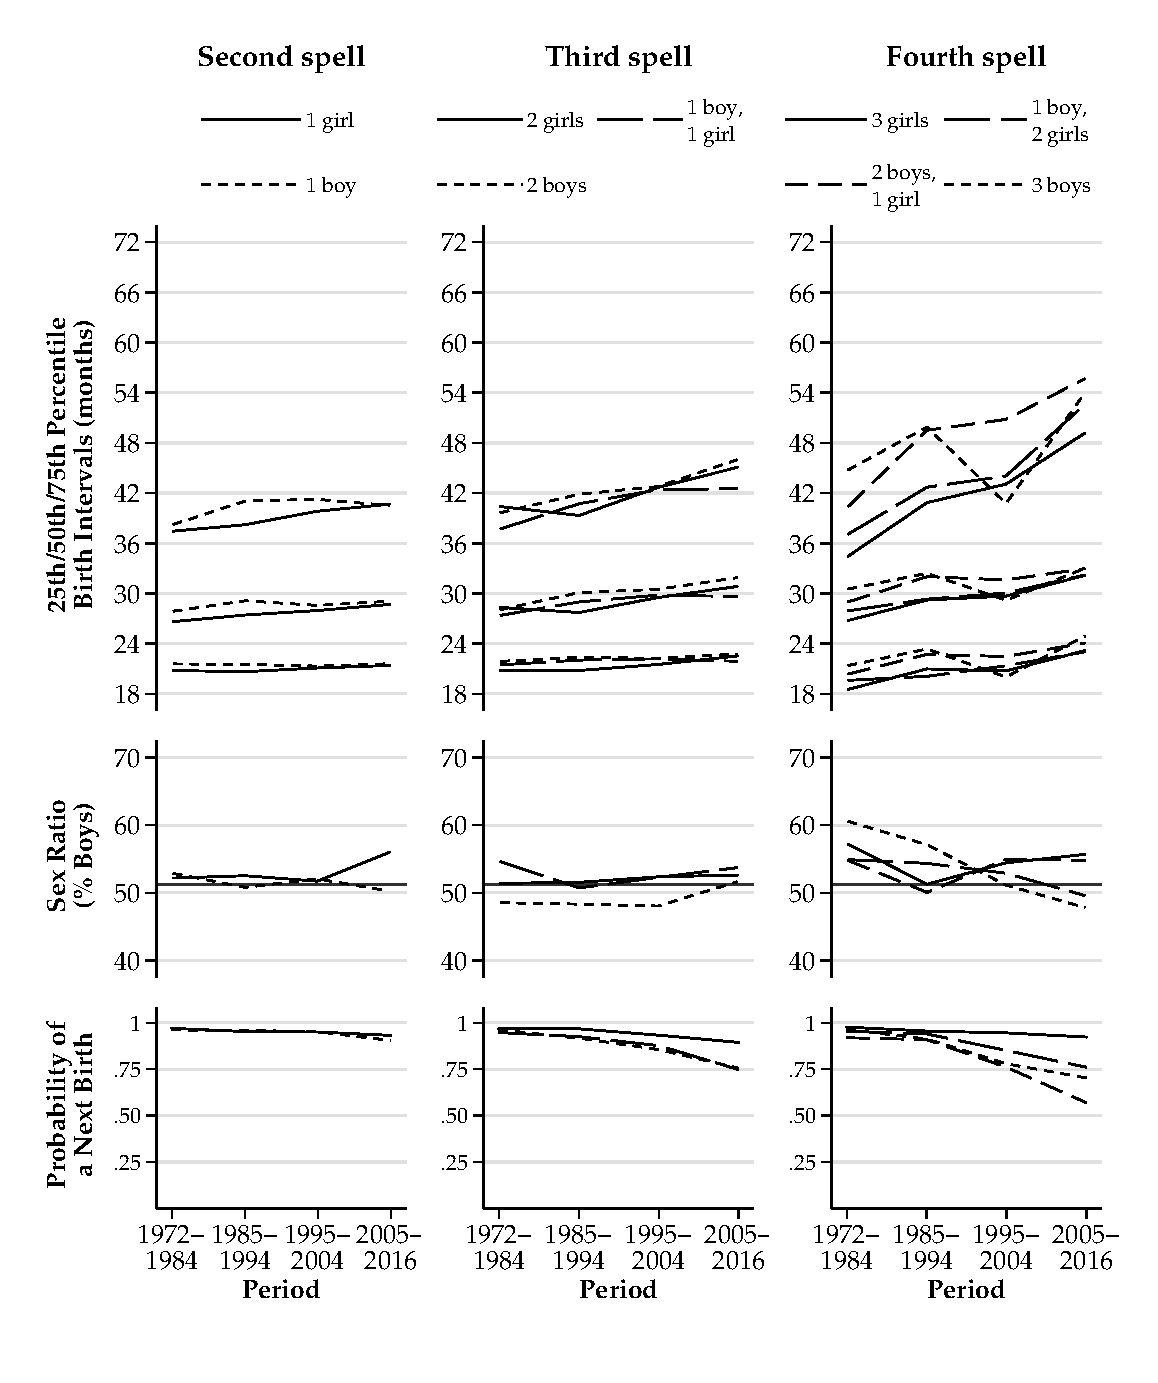
\includegraphics[width=\textwidth,height=\textheight,keepaspectratio=true]{bs_low_urban}
% \caption{Percentile birth intervals, sex ratios, and parity progression  
% for urban women with no education by spell, sex composition, and period}
% \label{fig:spacing_low_urban}
% \end{figure}

\begin{figure}
\centering
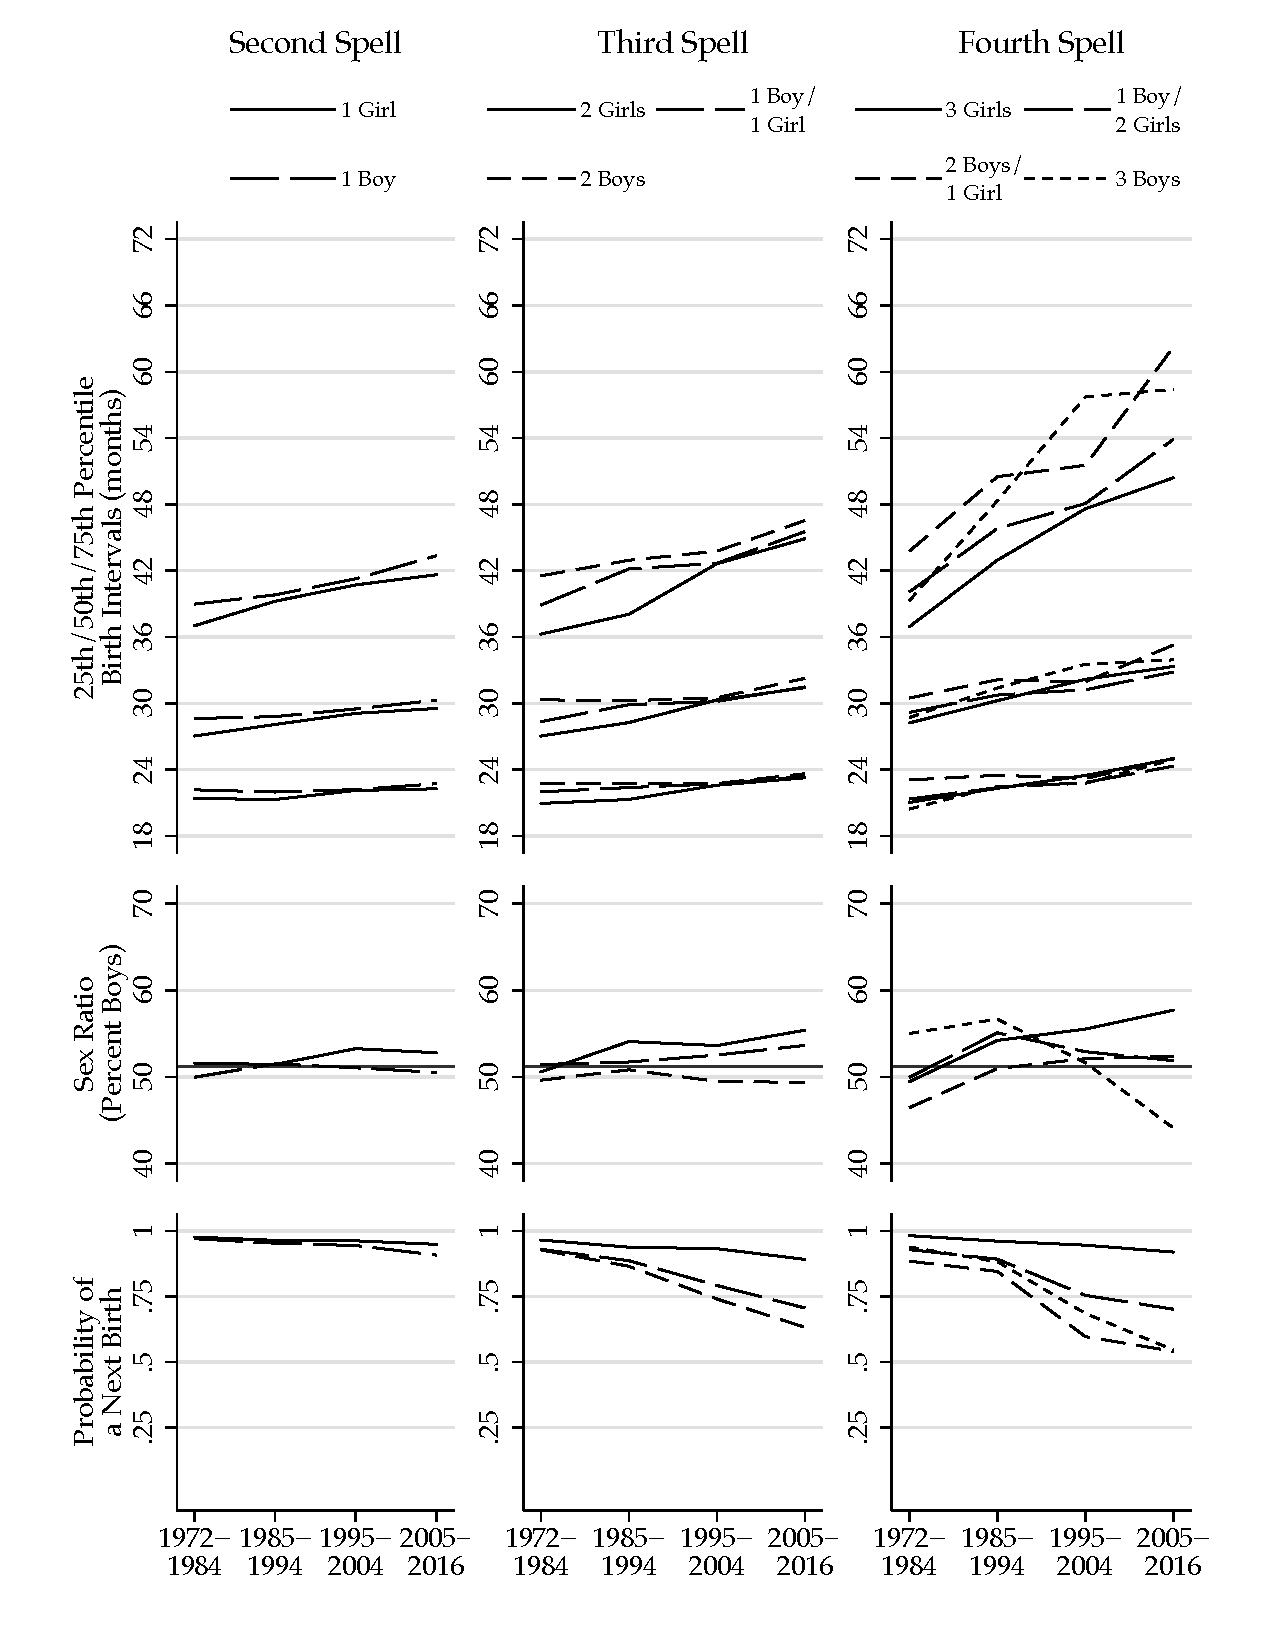
\includegraphics[width=\textwidth,height=\textheight,keepaspectratio=true]{bs_med_rural}
\caption{Percentile birth intervals, sex ratios, and parity progression  
for rural women with 1--7 years of education by spell, sex composition, and period}
\label{fig:spacing_med_rural}
\end{figure}

\begin{figure}
\centering
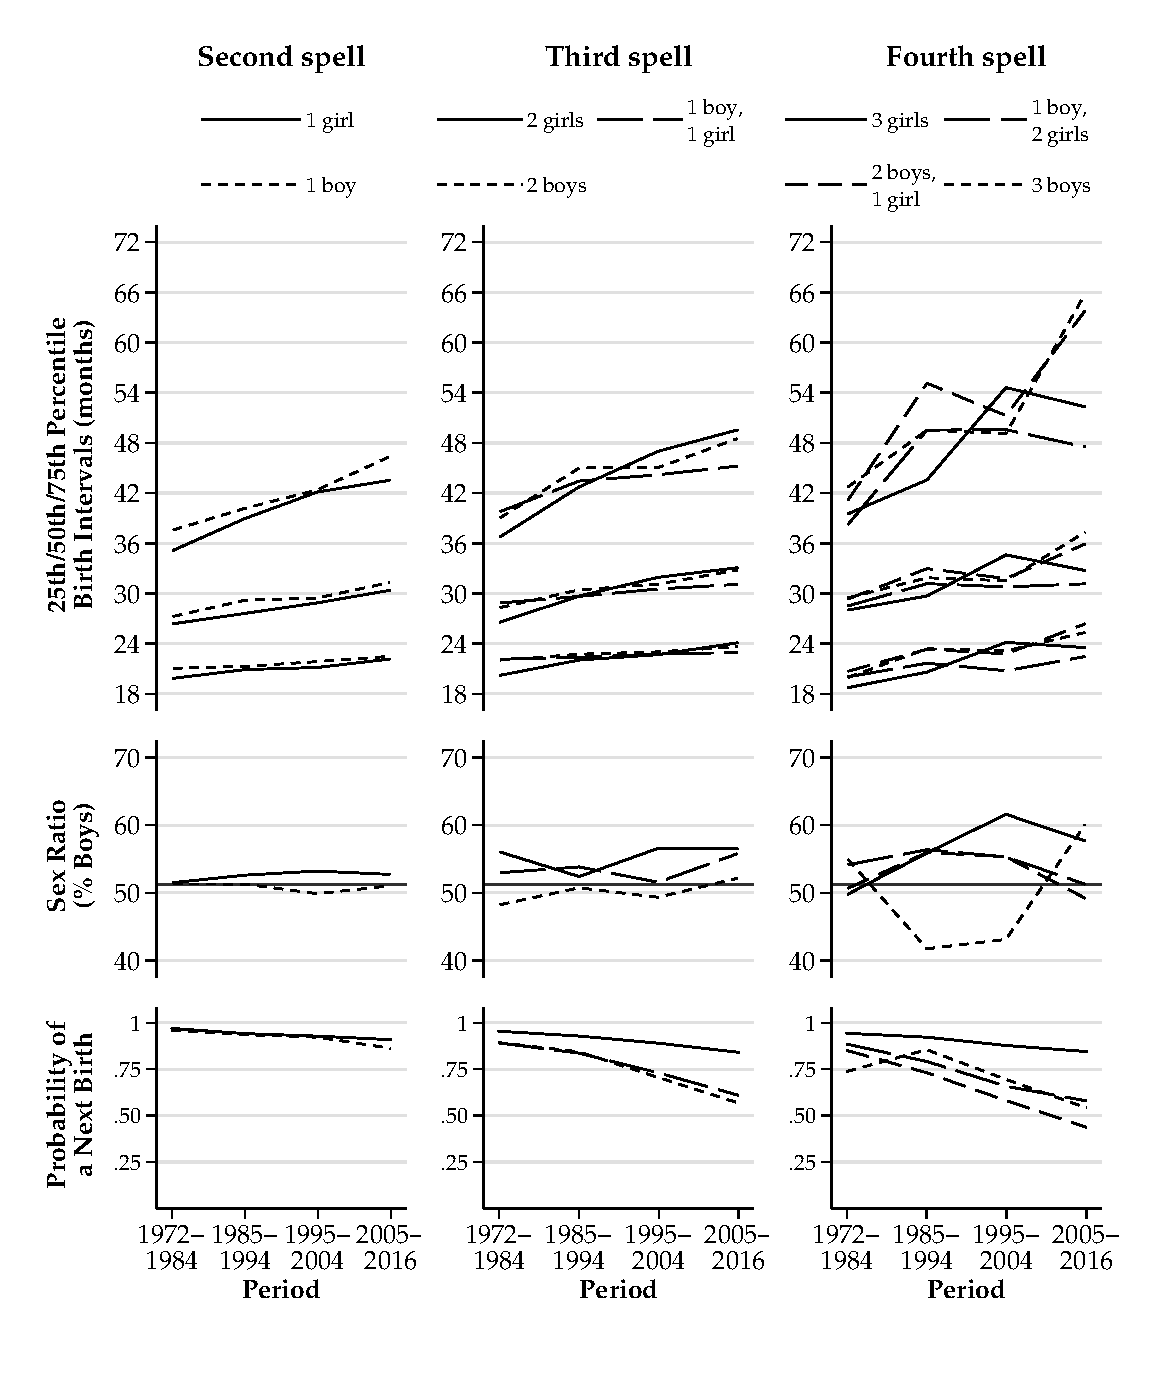
\includegraphics[width=\textwidth,height=\textheight,keepaspectratio=true]{bs_med_urban}
\caption{Percentile birth intervals, sex ratios, and parity progression  
for urban women with 1--7 years of education by spell, sex composition, and period}
\label{fig:spacing_med_urban}
\end{figure}

\begin{figure}
\centering
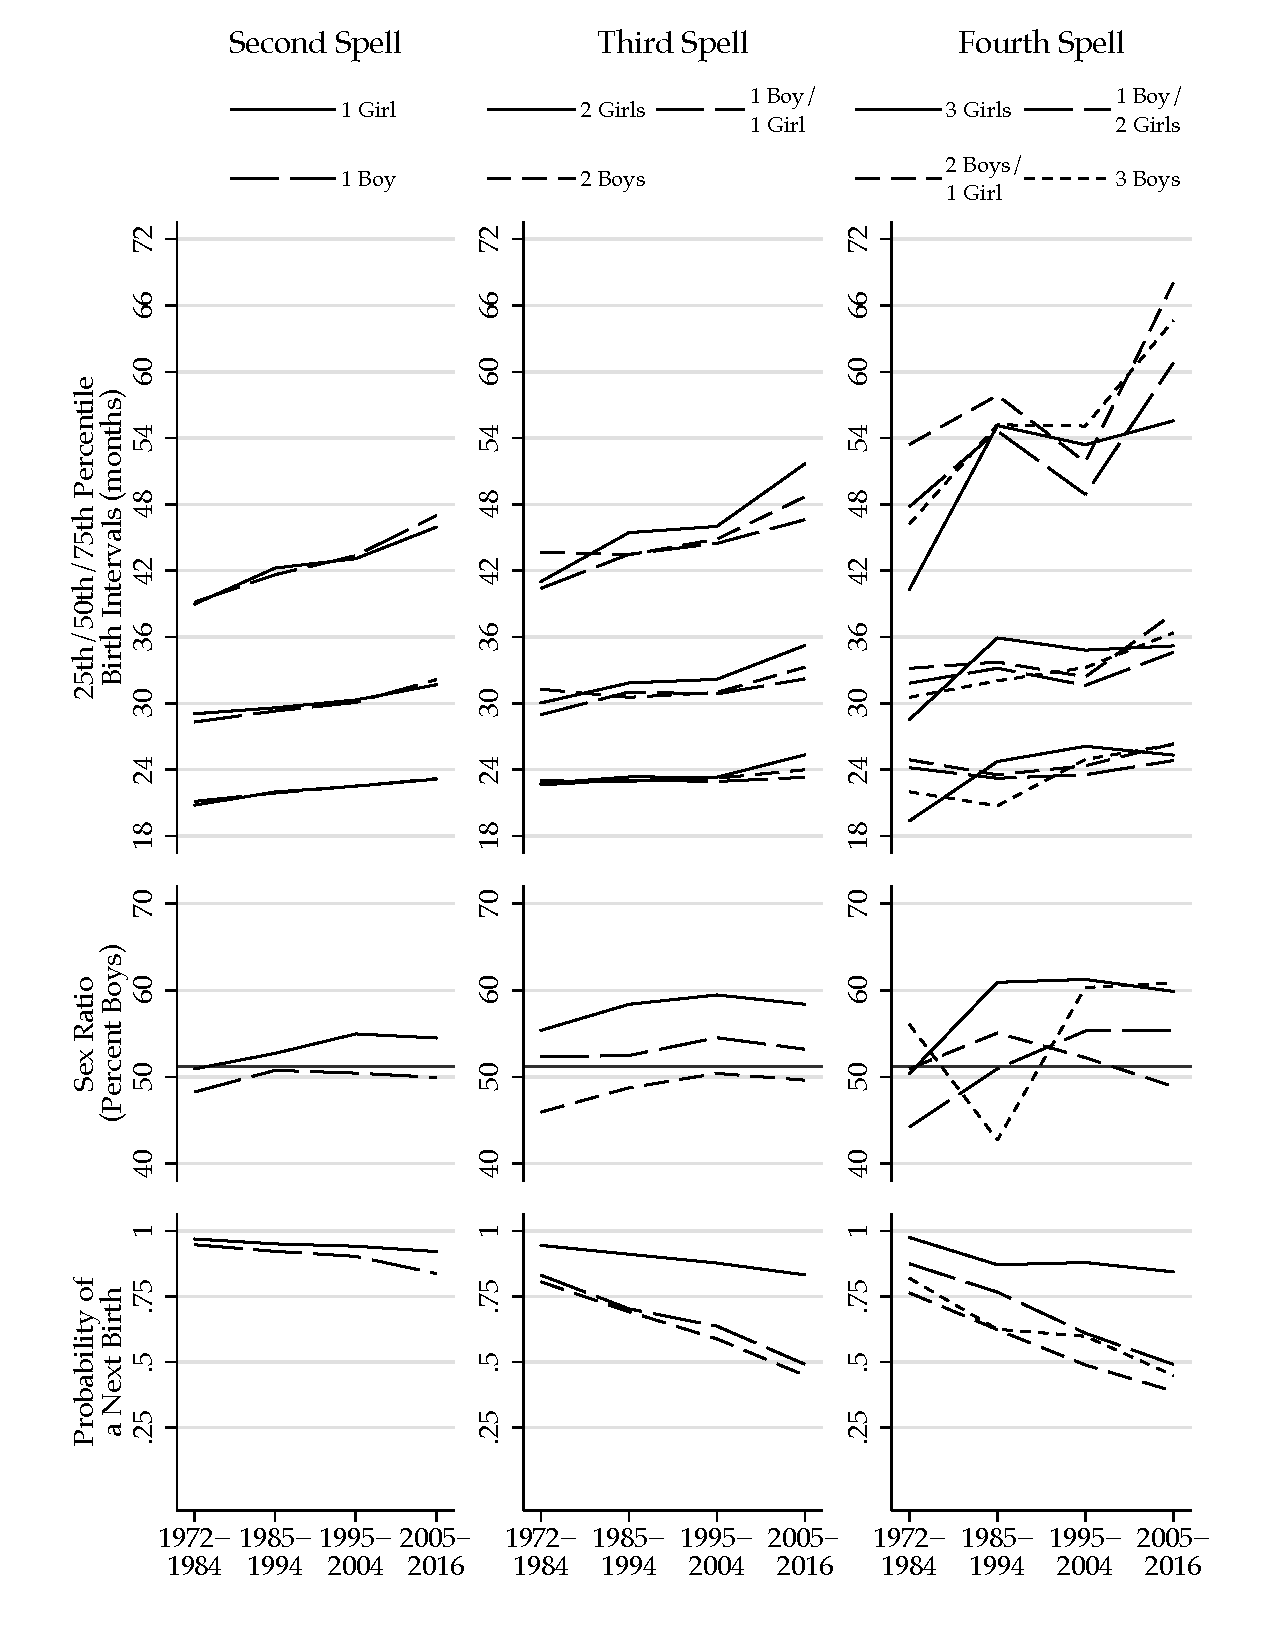
\includegraphics[width=\textwidth,height=\textheight,keepaspectratio=true]{bs_high_rural}
\caption{Percentile birth intervals, sex ratios, and parity progression  
for rural women with 8--11 years of education by spell, sex composition, and period}
\label{fig:spacing_high_rural}
\end{figure}

\begin{figure}
\centering
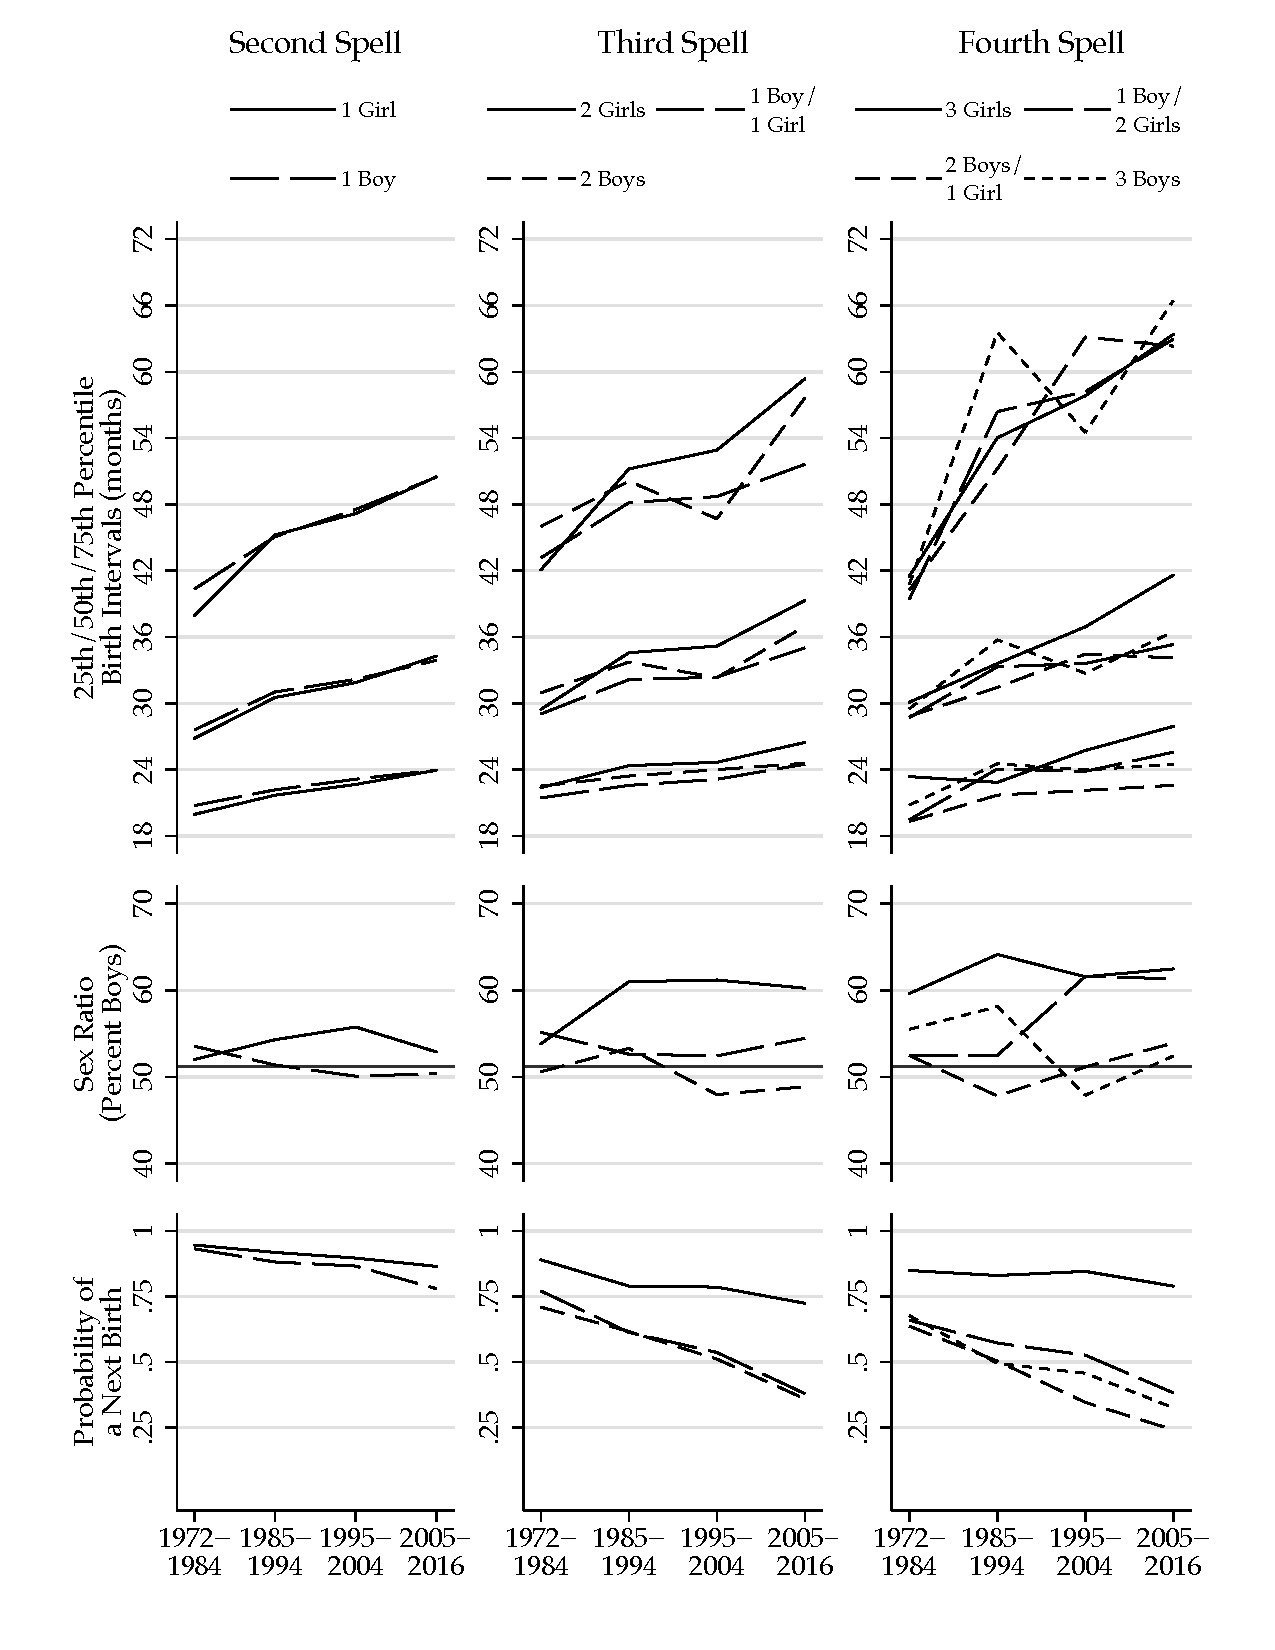
\includegraphics[width=\textwidth,height=\textheight,keepaspectratio=true]{bs_high_urban}
\caption{Percentile birth intervals, sex ratios, and parity progression  
for urban women with 8--11 years of education by spell, sex composition, and period}
\label{fig:spacing_high_urban}
\end{figure}

% \begin{figure}
% \centering
% 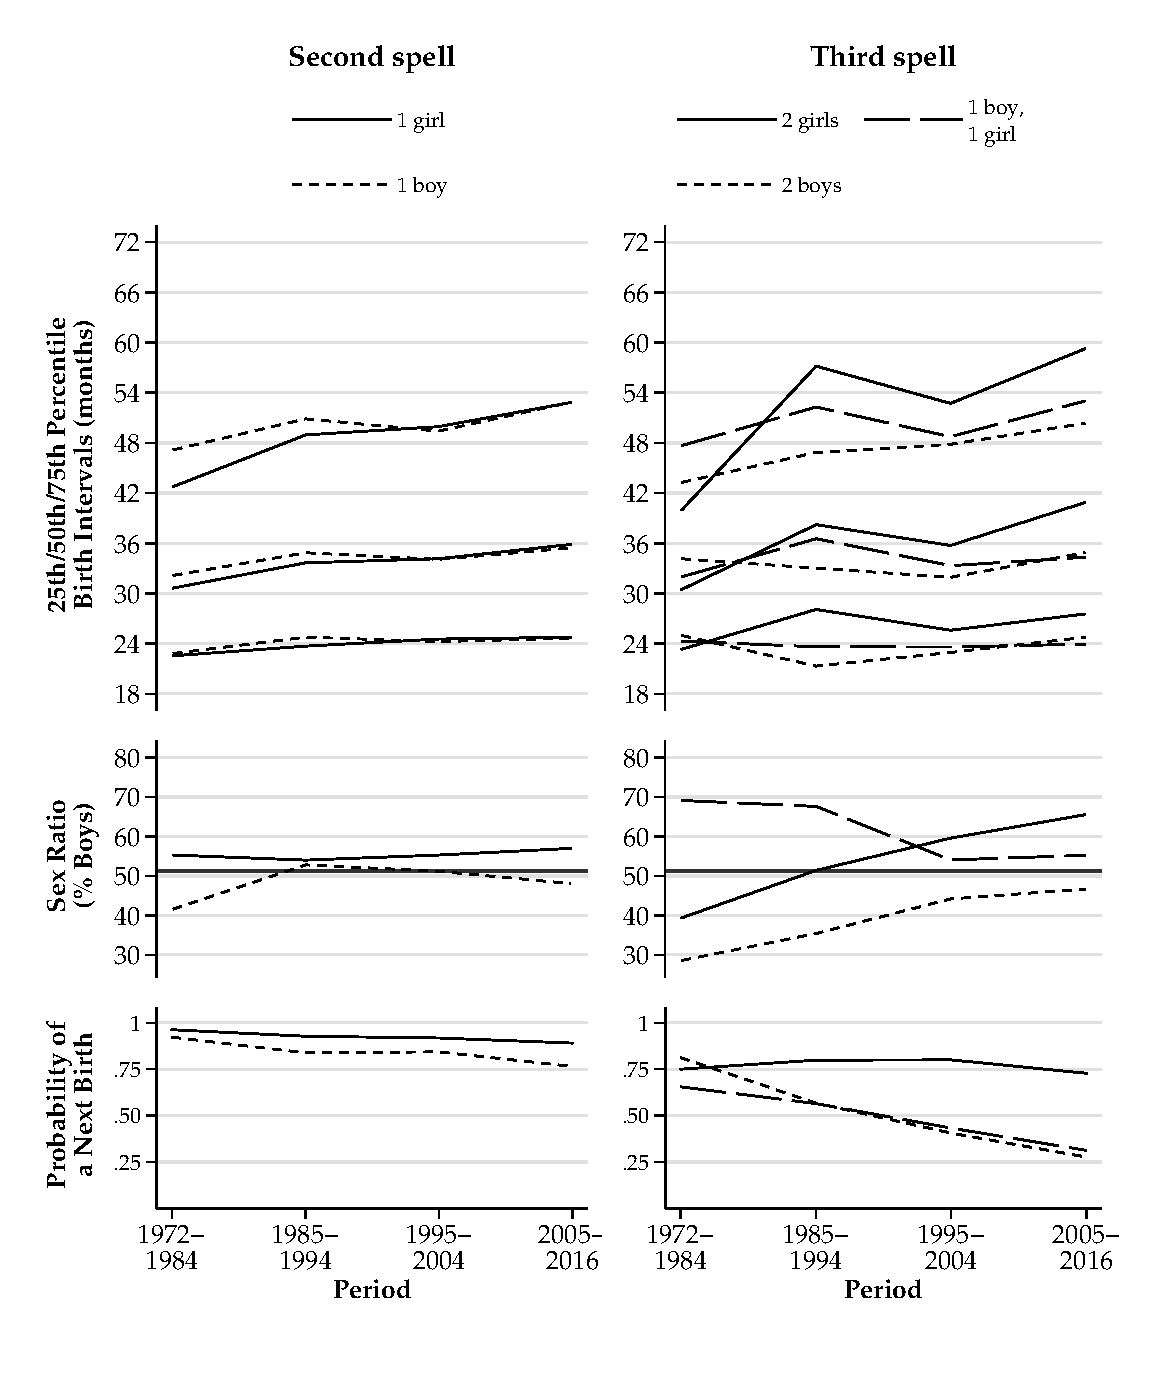
\includegraphics[width=\textwidth,height=\textheight,keepaspectratio=true]{bs_highest_rural}
% \caption{Percentile birth intervals, sex ratios, and parity progression  
% for rural women with 12 or more years of education by spell, sex composition, and period}
% \label{fig:spacing_highest_rural}
% \end{figure}

\begin{figure}
\centering
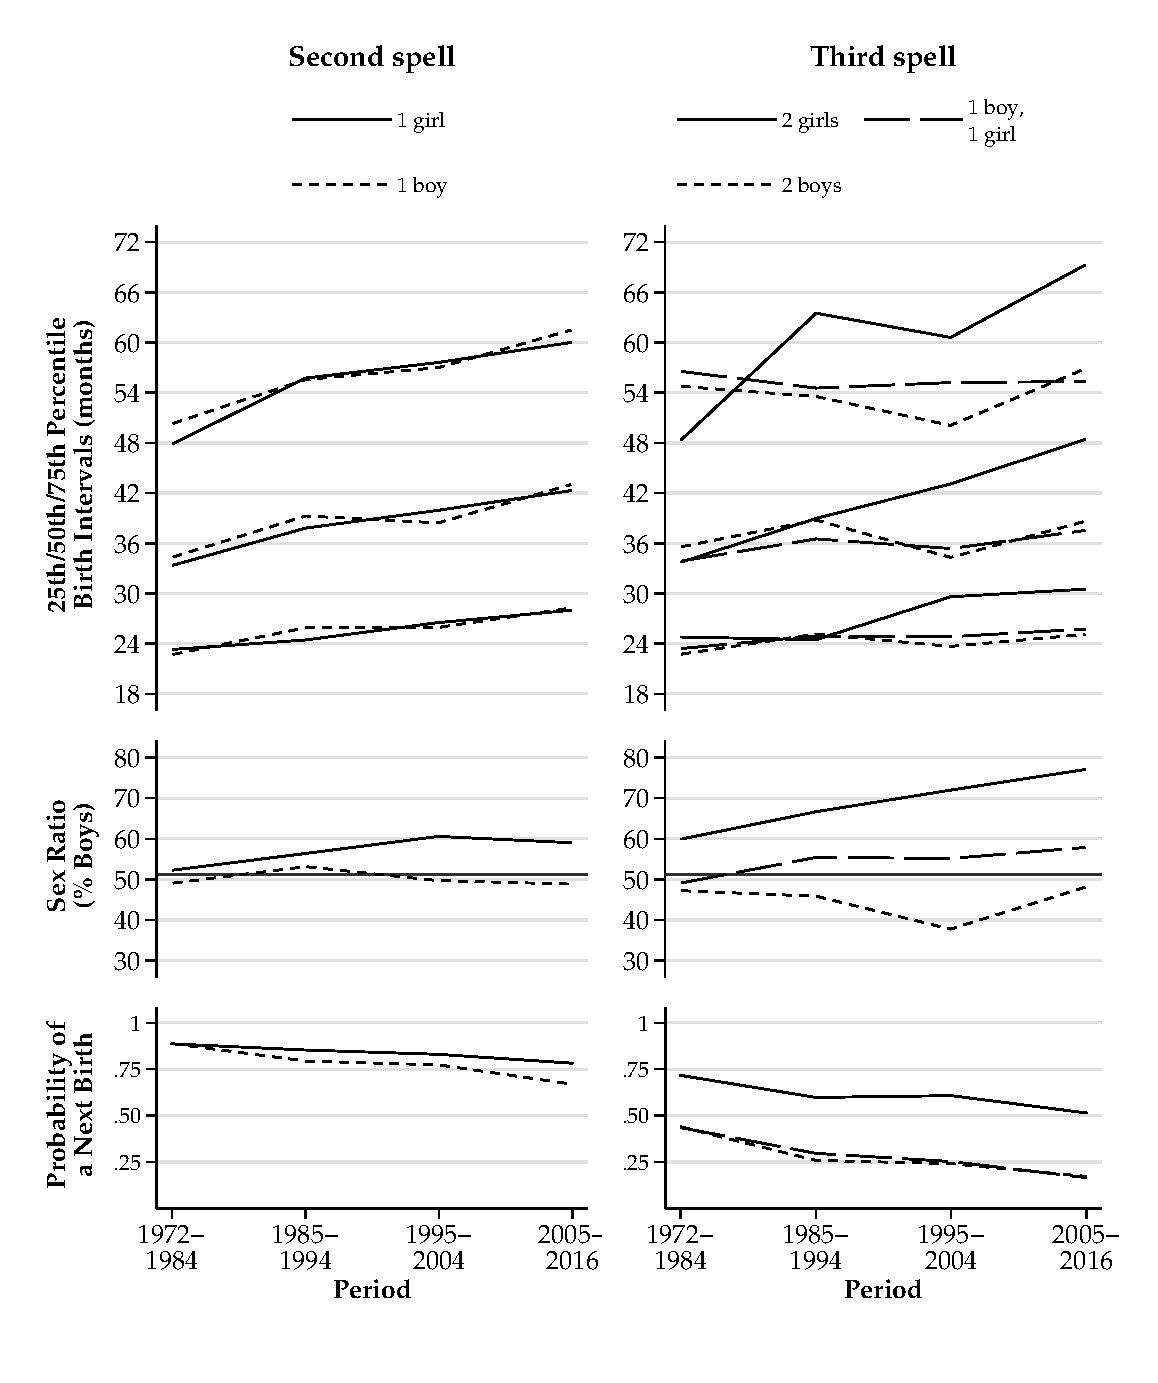
\includegraphics[width=\textwidth,height=\textheight,keepaspectratio=true]{bs_highest_urban}
\caption{Percentile birth intervals, sex ratios, and parity progression  
for urban women with 12 or more years of education by spell, sex composition, and period}
\label{fig:spacing_highest_urban}
\end{figure}


% [Parity progression probability]
The parity progression and the sex ratio show two broad trends.
First, 
in line with the falling total fertility rate, the likelihood of a next birth 
has decreased over time.
The likelihood of a next birth fell more rapidly, the higher the education, the higher the 
parity, and with at least one son.
Within a given spell and period, parity progressions are lower in urban than rural areas, 
if at least one son is present, and the more educated the mother.


% [Sex ratios]
Second, 
the spread of sex selection shows clearly in the sex ratios of next births, which has 
become more male-dominated for women with no sons.
The percentage of births that were boys increased more quickly, the higher the education and the 
higher the parity.
There are no clear trends for the other sex compositions.
Within a given spell and period combination and in the absence of a son, sex ratios are higher 
the more educated the mother is and with higher parity. 
Sex ratios are also higher in urban than in rural areas.
Some women with one son also show an unnaturally high percentage of boys, although the 
failing fertility makes these estimates noisy.


% [Birth intervals w/o sex selection]
\subsection{When Sex Selection Is Less Used}

To separate the effects of the introduction of sex selection and the other changes in
India, I first discuss how birth intervals have changed in situations where sex selection 
is less used.
The group broadly covers women with no education, regardless of the sex composition of their 
children, and women with any education who have one or two sons already. 
Despite the lower level of sex selection, son preference is still evident with the 
shortest spacing when they have only girls. 
Notably, for those least likely to use sex selection---rural women with no education---the 
difference in birth intervals across sex compositions has grown over time as spacing when 
sons are present has increased.

% [25th percentile birth intervals]
A remarkably high proportion of birth intervals are still very short.
For all but the most educated, 25\% or more have their second and third child 
within 24 months of the previous birth.
These intervals are substantially below the 24 months between 
\emph{pregnancies} the WHO recommends.
Furthermore, despite higher parities' more substantial increases in birth intervals, even 
the 25th percentile birth intervals for the fourth spell are around 24 months for women 
with less than eight years of education.

% [median birth intervals]
Median birth intervals have also increased relatively little---only three to six months 
over the four decades---compared to around 3.5 months \emph{per decade} in other countries with 
declining fertility \citep{Rutstein2011,Casterline2016}.%
\footnote{
The NFHS reports show median closed birth intervals of approximately 31 months, which have 
barely moved over time, underscoring the importance of accounting for censoring when examining 
birth spacing.
}
The result is that most of the median birth intervals are still at 36 months or below, 
with the shortest only 29 months.


Birth intervals appeared to lengthen the most for women the least likely to work.
For example, from lowest to highest education, the average third-spell birth intervals for 
urban women with one boy and one girl increased by 2.7, 3.4, 5.8, and 1.8 months over the 
four decades.%
\footnote{
For women with two sons, the numbers were 4.3, 6.3, 7.0, and 3.0.
See the online appendix tables for the average birth intervals.
}
Hence, women with the lowest labor force participation---those with 8--11 years 
of education---also saw the largest increases in average spacing, possibly driven by the 
substantial improvement in household income for this group from economic growth.


% [75th percentile birth intervals]
The most substantial changes occurred in the 75th percentile birth intervals, where the 
more the parity progression probabilities declined, the more the birth interval lengthened. 
For example, the probability of a fourth birth for urban women with 8--11 years 
of education and two sons and a girl has declined by almost 40 percentage points as the 
75th percentile birth interval increased by 22 months.
Compare this with rural women of no education with a boy as their first child, for whom the 
probability of a third birth declined by fewer than six percentage points while the birth 
interval increased only slightly over two months.

%0.637 0.241

These results are in line with prior research showing that falling fertility is associated 
with increases in longer spacing, although why is still an unresolved question 
\citep{Casterline2016}.
The exception to this trend suggests one possible answer.
For the most educated women who already have a son, the probability of a third birth 
declined rapidly, but the birth intervals changed little.
These women both have better access to modern contraceptives and are better at using 
traditional contraceptive methods \citep{Rosenzweig1989}.


% [Interpretation]
% How do these changes in birth intervals tie in with the changes in India over the four
% decades?
% [TK economic growth? -> higher return to education for males -> lower fertility and
% higher investment in boys' education -- has anybody looked at this?]
% First, the parity progression probabilities have been falling over time across all 
% education levels, especially for women with at least one son.



% [Birth intervals with sex selection]
\subsection{Sex Selection and Birth Spacing}

A clear illustration of how the combination of son preference and the introduction of 
sex selection affected birth spacing comes from the third spell of the best-educated urban 
women.
With two girls, almost 80\% of the third births are boys, and the 75th percentile 
birth interval is close to 70 months. 
This interval is about 13 months longer than if they had at least one son and represents 
an increase of almost 21 months over the four decades.

Even more striking is that most of the change took place right at the introduction of sex 
selection.
The 75th percentile birth interval with two girls increased from 48 months to 
64 months in a decade, while the other sex compositions showed a slight decrease from 
around 55 months to 54 months.
These changes in birth spacing may even be an underestimate because this particular group 
appears to have had access to sex selection even before it became widespread, as shown by 
the unequal sex ratio for the 1972--1984 period for women with two girls.


The 75th percentile changes are the most dramatic, but sex selection also affects the 
25th and median birth intervals. 
For the best-educated urban women with two girls, the 25th percentile birth interval 
increased by six months, or 23\%, while the median percentile birth interval 
increased by 15 months (43\%).


Not surprisingly, given these effects of sex selection, the third spell for the 
best-educated women shows the clearest reversal in the spacing pattern; 
the birth intervals with two girls are consistently longer than the intervals with one or 
two boys, no matter the percentile used.
A similar reversal, although more muted, occurred for the third spell for urban women 
with 1--7 years of education and both urban and rural women with 8--11 years of 
education.

% An important exception to the relatively short median intervals come from the better 
% educated women, especially in the absence of sons.
% The longest median interval was 48 months for the third spell for urban women with twelve 
% or more years of education who had no boys, an increase of almost 15 months over
% four decades.
% Similary, urban women with eight to eleven years of education and no sons had median
% birth intervals of around 40 months, an increase of about 10 months.
% Finally, the best educated women now have a median second birth interval of around 42
% months whether their first child was a boy or a girl.


% Despite the strong son preference in spacing and sex ratios, there is also some indication 
% that parents prefer a mix of boys and girls;
% women with two boys \emph{and} a girl consistently have the lowest parity progression 
% probability in the fourth spell across education levels. 

Did the predictions of declining use of sex selection come true? 
There is no clear evidence for or against a reversal in the use of sex selection, with 
some cases showing increases in sex ratios between the last two periods, others little 
change, and some a decline. 
The best-educated women are again a good illustration. 
The sex ratio for women with two girls continued to increase over the last two periods, 
but the likelihood of a third birth declined. 
Furthermore, if the first child was a girl, the sex ratio for the second birth dropped 
slightly, as did the probability of having a second birth. 
However, there are also cases where there is no abatement in the increasing use of sex 
selection. 
For example, for rural women with 1--7 years of education, the sex ratios in the 
absence of girls continued to increase while the likelihood of an additional birth remained 
high.


In summary, over the four decades, birth intervals lengthened with improving economic 
conditions and falling fertility. 
These increases are larger with higher parity and higher percentile measure. 
Furthermore, when sex selection is less used, it appears that the women least likely to 
work are also those with the most substantial increases.

Sex selection, however, is behind the most substantial increases in birth spacing. 
The best-educated women with two girls had the most biased sex ratio and the most 
significant increase in birth intervals. 
Over the four decades, the median birth interval for this group increased by almost 15 
months, 
and the 75th percentile birth interval increased by a staggering 21 months, most of that 
within a decade.

\section{What Happened to Fertility?\label{sec:fertility}}

The tempo effect from longer birth intervals means that the total fertility rate may 
underestimate cohort fertility. 
The next question I address is, therefore, to what extent did the changes bias the 
fertility estimates for India? 
To this end, I compare fertility based on a variation of the total fertility rate with 
predicted cohort fertility from the hazard model.
Table \ref{tab:fertility} shows the two fertility measures by area of residence and education.

\begin{table}[hp!]
\begin{center}
\begin{footnotesize}
\begin{threeparttable}
\caption{Four-parity fertility rate versus predicted cohort fertility based on hazard model}
\label{tab:fertility}
\begin{tabular}{@{} l D{.}{.}{2.2} D{.}{.}{2.2} D{.}{.}{2.2} D{.}{.}{2.2} D{.}{.}{2.2}  @{}}
\toprule
                       &            \mct{NFHS--1}          & \mco{NFHS--2}   & \mco{NFHS--3}   & \mco{NFHS--4}   \\
Fertility Rate Period  & \mco{1987--1988}  & \mco{1992--1993}  & \mco{1998--1999}  & \mco{2005--2006}  & \mco{2015--2016}  \\
Hazard Model Period    & \mco{1972--1984}  &                 & \mco{1985--1994}  & \mco{1995--2004}  & \mco{2004--2016}  \\
\midrule
 & \multicolumn{5}{c}{Urban} \\ \cmidrule(lr){2-6}
 & \multicolumn{5}{c}{No Education} \\
Fertility Rate\tnote{a}   &      3.55       &      3.06       &      2.80       &      2.54       &      2.45       \\
Hazard Model\tnote{b}     &      3.44       &                 &      3.29       &      3.06       &      2.79       \\
\addlinespace 
 & \multicolumn{5}{c}{1--7 Years of Education} \\
Fertility Rate\tnote{a}   &      2.85       &      2.29       &      2.09       &      1.99       &      2.04       \\
Hazard Model\tnote{b}     &      3.18       &                 &      2.88       &      2.62       &      2.42       \\
\addlinespace 
 & \multicolumn{5}{c}{8--11 Years of Education} \\
Fertility Rate\tnote{a}   &      2.43       &      2.04       &      1.84       &      1.81       &      1.87       \\
Hazard Model\tnote{b}     &      2.72       &                 &      2.41       &      2.28       &      2.07       \\
\addlinespace 
 & \multicolumn{5}{c}{12 or More Years of Education} \\
Fertility Rate\tnote{a}   &      2.05       &      1.68       &      1.57       &      1.55       &      1.51       \\
Hazard Model\tnote{b}     &      2.29       &                 &      2.06       &      1.94       &      1.80       \\
\addlinespace 
 & \multicolumn{5}{c}{Rural} \\ \cmidrule(lr){2-6}
 & \multicolumn{5}{c}{No Education} \\
Fertility Rate\tnote{a}   &      3.57       &      2.93       &      2.63       &      2.74       &      2.81       \\
Hazard Model\tnote{b}     &      3.55       &                 &      3.38       &      3.26       &      3.09       \\
\addlinespace 
 & \multicolumn{5}{c}{1--7 Years of Education} \\
Fertility Rate\tnote{a}   &      3.01       &      2.52       &      2.39       &      2.25       &      2.37       \\
Hazard Model\tnote{b}     &      3.29       &                 &      3.08       &      2.83       &      2.70       \\
\addlinespace 
 & \multicolumn{5}{c}{8--11 Years of Education} \\
Fertility Rate\tnote{a}   &      2.56       &      2.21       &      2.22       &      2.16       &      2.19       \\
Hazard Model\tnote{b}     &      2.93       &                 &      2.68       &      2.49       &      2.31       \\
\addlinespace 
 & \multicolumn{5}{c}{12 or More Years of Education} \\
Fertility Rate\tnote{a}   &      1.95       &      1.68       &      2.13       &      2.08       &      1.96       \\
Hazard Model\tnote{b}     &      2.64       &                 &      2.39       &      2.25       &      2.11       \\
\addlinespace 
\bottomrule
\end{tabular}
\begin{tablenotes} \scriptsize
\item \hspace*{-0.5em} \textbf{Note.}
All predictions based on births up to and including parity four births
for both fertility rate and model predictions.
NFHS-1 was collected in 1992--1993, and model results for 1972--1984 were
applied for the predictions.
NFHS-2 was collected in 1998--1999, and model results for 1985--1994 were
applied for the predictions.
NFHS-3 was collected in 2005--2006, and model results for 1995--2004 were
applied for the predictions.
NFHS-4 was collected in 2015--2016, and model results for 2005--2016 were
applied for the predictions.
\item[a] 
The fertility rate is based on five-year age groups, counting births that 
occurred 1--36 months before the survey months.
For NFHS-1 and NFHS-2, the total number of women in the five-year age
groups is based on the household roster because only ever-married women
are in the individual recode sample.
For NFHS-3 and NFHS-4, the total number of women is based on the individual
recode sample because all women were interviewed.
\item[b] 
The model predictions for fertility are the average predicted fertility
across all women in a given sample, using their age of marriage as the
starting point and adding three years for each spell.
Observed births are not taken into account for the predictions.
For each spell, the predicted probability is the likelihood of having a
next birth given sex composition multiplied with the probability of that
sex composition and the likelihood of getting to the spell,
corrected for the probability of sterilization.
\end{tablenotes}
\end{threeparttable}
\end{footnotesize}
\end{center}
\end{table}


The fertility rate follows the same procedure as in the Demographic and Health Survey 
reports: I use the births from 36 to 1 month before the survey month to calculate 
age-specific fertility rates for five-year age groups and then sum the age-specific 
fertility rates multiplied by five  \citep{Croft2018}.
However, because the hazard model predictions only use births up to parity four, I use the 
same set of births for the fertility rate and label it the ``four-parity'' fertility rate. 
Hence, the presented fertility rates are not directly comparable to those in the NFHS reports.

%
% \footnote{
% See \citet{Croft2018} for more detail.
% Because NFHS-1 and NFHS-2 did not interview all women about fertility, the number of women 
% is based on the household rosters, assuming that never-married women have had no children.
% Because of the low number of births to women aged 45 to 49 this age group was not
% used for the hazard model estimations and, therefore, is also excluded for the fertility
% rate.
% The marital total fertility rate lead to unrealistically high numbers and is, therefore,
% not presented \citep{Hoem2011,Laplante2015}.
% }

Because NFHS-1 was after the introduction of sex selection, I cannot calculate a fertility 
rate in precisely the same manner for a period before sex selection was widely available.
Instead, I calculate the fertility rates for women between 15 and 39 years of age five years 
before the survey month, again using the number of births three years before.
This rate is shown as ``1987--1988'' in the table.
Given the relatively low number of births to women 40--45 years of age, this approach 
provides the best estimate of the fertility rate when sex selection still was not 
widespread.

To predict cohort fertility based on the hazard models, I estimate the parity progression 
probability for each spell. 
Because parity progression depends on the sex composition of prior children, I estimate the 
probability for each sex composition and weigh the probabilities with the likelihood of 
the sex compositions.
The survey rounds do not coincide directly with the periods used for the hazard model.
Therefore, I compare the model results for 1972--1984, 1985--1994, 1995--2004,
and 2005--2016 with rounds 1 through 4 of the NFHS, respectively.

I include the spell from marriage to first birth, despite the problems capturing the exact 
timing of marriages because the estimated progression probabilities should not be affected 
by this problem. 
I begin with the age of marriage for each woman and predict the likelihood of progressing 
to each parity, assuming three-years increases in age between births. 
Shorter assumed increases in age lead to slightly higher predicted fertility.

Sterilizations are not incorporated into the hazard model because most occur
immediately after giving birth. 
To compensate, I estimate the probability of sterilization using a Logit model and use 
that to scale down the parity progression probability when predicting cohort fertility.

The predicted cohort fertility based on the hazard model is higher than the four-parity 
fertility rate in almost all cases. 
Only women with no education in the first period show little difference between the two 
fertility measures, a situation where fertility is high, spacing very short, and likely 
unchanged for an extended period.

Consistent with a more substantial bias in the fertility rate when the age of marriage 
and the length of birth intervals increase, the absolute bias is least in the first 
and the last period and highest in the middle two periods.
Hence, the fertility rate declined too fast from the mid-1980s to the century's end.
Only recently, as the rate of increase for the birth intervals has slowed, have the two 
fertility measures begun to converge again.
Even with the convergence, the predicted 2005--2016 cohort fertility is still above the 
1992--1993 fertility rate for every group, except urban women with no education. 
Furthermore, for the last period, the predicted cohort fertility remains at least 
10\%--20\% higher than the fertility rate.

Another indication of how tempo effects bias the fertility rate bias is that the
fertility rate \emph{increases} for some groups.
For example, for urban women with 8--11 years of education, the fertility
rates were 1.84, 1.81, and 1.87 over the last three surveys.
This pattern likely arises from the stabilization of the age of first birth and the 
spacing between births.

Finally, even with the declines in the predicted cohort fertility, it is still mostly 
above replacement.
Only for urban women with 12 or more years of education is the predicted cohort
fertility clearly below 2.1 children.
Even then, cohort fertility is still more than 0.3 children higher than 
the fertility rate estimate of 1.5.
Furthermore, the predicted cohort fertility numbers are likely too low because I use only 
the first four births and births before the imposed 105-month birth interval censoring.


\section{Mortality and the Changing Birth Spacing\label{sec:mortality}}

The final question I address is whether there is an association between infant mortality 
and increases in birth spacing and sex selection. 
Starting with the sample used for estimating birth spacing, I select children born more 
than 12 months before the survey month. 
I restrict the analyses to parities two and three because of the small number of births 
and deaths for parity four. 
Furthermore, I do not show the results for women with 12 or more years of education 
for the 1972--1984 period because of the small number of women.

The dependent variable is whether the child died within the first 12 months of life.
The main set of explanatory variables consists of dummies for the spacing from
the prior birth.
The birth interval dummies cover 12-month periods, starting nine months after the prior 
birth, until the 57-month dummy, which covers until 105 months after the prior birth.
I use dummies for sex of the index child and the sex composition 
of the prior children.
The birth spacing dummies, the sex of index child, and the sex composition dummies
are all interacted.
Because the actual number of abortions is unobserved, the interactions between
the sex composition of prior children and the sex of the index child serve
as proxies for the use of sex selection.
The other explanatory variables are the same as above, and estimations
are done separately by education level and parity.

I estimate the probability of infant mortality using a Logit model.
Figures \ref{fig:mortality_low_med} and \ref{fig:mortality_high_highest} show 
the predicted probability of the second child dying within the first year at the 
possible combinations of index child sex, sex composition of prior children, and 
birth spacing, with all other variables at their average values.%
\footnote{
The online appendix shows the corresponding graphs for the third child.
}
The graphs do not show confidence intervals to improve legibility.

An important caveat is that the estimations do not 
address potential selection problems.
For example, suppose women who have difficulties conceiving or carrying a pregnancy to 
term also have a higher mortality risk for their offspring. 
In that case, a spurious correlation between long birth spacing and mortality may arise 
\citep{Kozuki2013}. 
Unfortunately, methods to address selection, such as family fixed effects, do not work 
well when the number of births is as low as for better-educated women 
\citep{Kozuki2013,Molitoris2019}.
However, the fixed effects and linear probability results did not 
deviate substantially in prior research.


% \begin{figure}[htpb]
% \centering
% \rotatebox[origin=c]{90}{\small{1972-1984}}
% \setcounter{subfigure}{-1}
% \subfloat[Second Spell]{
%     \begin{minipage}{0.37\textwidth}
%         \captionsetup[subfigure]{font=footnotesize,labelformat=empty,position=top,captionskip=-1pt,farskip=-0.5pt}
%         \subfloat[No Eduction]{\includegraphics[width=\textwidth]{mortality_s2_p1_low_dummies}}
%         \captionsetup[subfigure]{labelformat=parens}
%     \end{minipage}
% }
% \setcounter{subfigure}{-0} 
% \subfloat[Second Spell]{
%     \begin{minipage}{0.37\textwidth}
%         \captionsetup[subfigure]{font=footnotesize,labelformat=empty,position=top,captionskip=-1pt,farskip=-0.5pt}
%         \subfloat[One to Seven Years of Education]{\includegraphics[width=\textwidth]{mortality_s2_p1_med_dummies}}
%         \captionsetup[subfigure]{labelformat=parens}
%     \end{minipage}
% }
% \\
% \rotatebox[origin=c]{90}{\small{1985-1994}}
% \subfloat[Second Spell]{
%     \begin{minipage}{0.37\textwidth}
%         \includegraphics[width=\textwidth]{mortality_s2_p2_low_dummies}
%     \end{minipage}
% } 
% \subfloat[Second Spell]{
%     \begin{minipage}{0.37\textwidth}
%         \includegraphics[width=\textwidth]{mortality_s2_p2_med_dummies} 
%     \end{minipage}
% } 
% \\
% \rotatebox[origin=c]{90}{\small{1995-2004}}
% \subfloat[Second Spell]{
%     \begin{minipage}{0.37\textwidth}
%         \includegraphics[width=\textwidth]{mortality_s2_p3_low_dummies}
%     \end{minipage}
% } 
% \subfloat[Second Spell]{
%     \begin{minipage}{0.37\textwidth}
%         \includegraphics[width=\textwidth]{mortality_s2_p3_med_dummies} 
%     \end{minipage}
% } 
% \\
% \rotatebox[origin=c]{90}{\small{2005-2016}}
% \subfloat[Second Spell]{
%     \begin{minipage}{0.37\textwidth}
%         \includegraphics[width=\textwidth]{mortality_s2_p4_low_dummies}
%     \end{minipage}
% } 
% \subfloat[Second Spell]{
%     \begin{minipage}{0.37\textwidth}
%         \includegraphics[width=\textwidth]{mortality_s2_p4_med_dummies} 
%     \end{minipage}
% } 
% \caption{Predicted Probability of Second Child's Infant Mortality 
% for Women with No Education
% and Women with One to Seven Years of Education}
% \label{fig:mortality_low_med}
% \end{figure}


% \begin{figure}[htpb]
% \centering
% \rotatebox[origin=c]{90}{\small{1972-1984}}
% \setcounter{subfigure}{-1}
% \subfloat[Second Spell]{
%     \begin{minipage}{0.37\textwidth}
%         \captionsetup[subfigure]{font=footnotesize,labelformat=empty,position=top,captionskip=-1pt,farskip=-0.5pt}
%         \subfloat[Eight to Eleven Years of Education]{\includegraphics[width=\textwidth]{mortality_s2_p1_high_dummies}}
%         \captionsetup[subfigure]{labelformat=parens}
%     \end{minipage}
% }
% \begin{minipage}[t]{0.39\textwidth}\vspace{-2.68cm}\centering\footnotesize{Twelve or More Years of Education}\end{minipage}
% \\
% \rotatebox[origin=c]{90}{\small{1985-1994}}
% \subfloat[Second Spell]{
%     \begin{minipage}{0.37\textwidth}
%         \includegraphics[width=\textwidth]{mortality_s2_p2_high_dummies}
%     \end{minipage}
% } 
% \subfloat[Second Spell]{
%     \begin{minipage}{0.37\textwidth}
%         \includegraphics[width=\textwidth]{mortality_s2_p2_highest_dummies}
%     \end{minipage}
% } 
% \\
% \rotatebox[origin=c]{90}{\small{1995-2004}}
% \subfloat[Second Spell]{
%     \begin{minipage}{0.37\textwidth}
%         \includegraphics[width=\textwidth]{mortality_s2_p3_high_dummies}
%     \end{minipage}
% } 
% \subfloat[Second Spell]{
%     \begin{minipage}{0.37\textwidth}
%         \includegraphics[width=\textwidth]{mortality_s2_p3_highest_dummies} 
%     \end{minipage}
% } 
% \\
% \rotatebox[origin=c]{90}{\small{2005-2016}}
% \subfloat[Second Spell]{
%     \begin{minipage}{0.37\textwidth}
%         \includegraphics[width=\textwidth]{mortality_s2_p4_high_dummies}
%     \end{minipage}
% } 
% \subfloat[Second Spell]{
%     \begin{minipage}{0.37\textwidth}
%         \includegraphics[width=\textwidth]{mortality_s2_p4_highest_dummies} 
%     \end{minipage}
% } 
% \caption{Predicted Probability of Second Child's Infant Mortality 
% for Women with Eight to Eleven of Education
% and Women with Twelve or More Years of Education}
% \label{fig:mortality_high_highest}
% \end{figure}


\begin{figure}
\centering
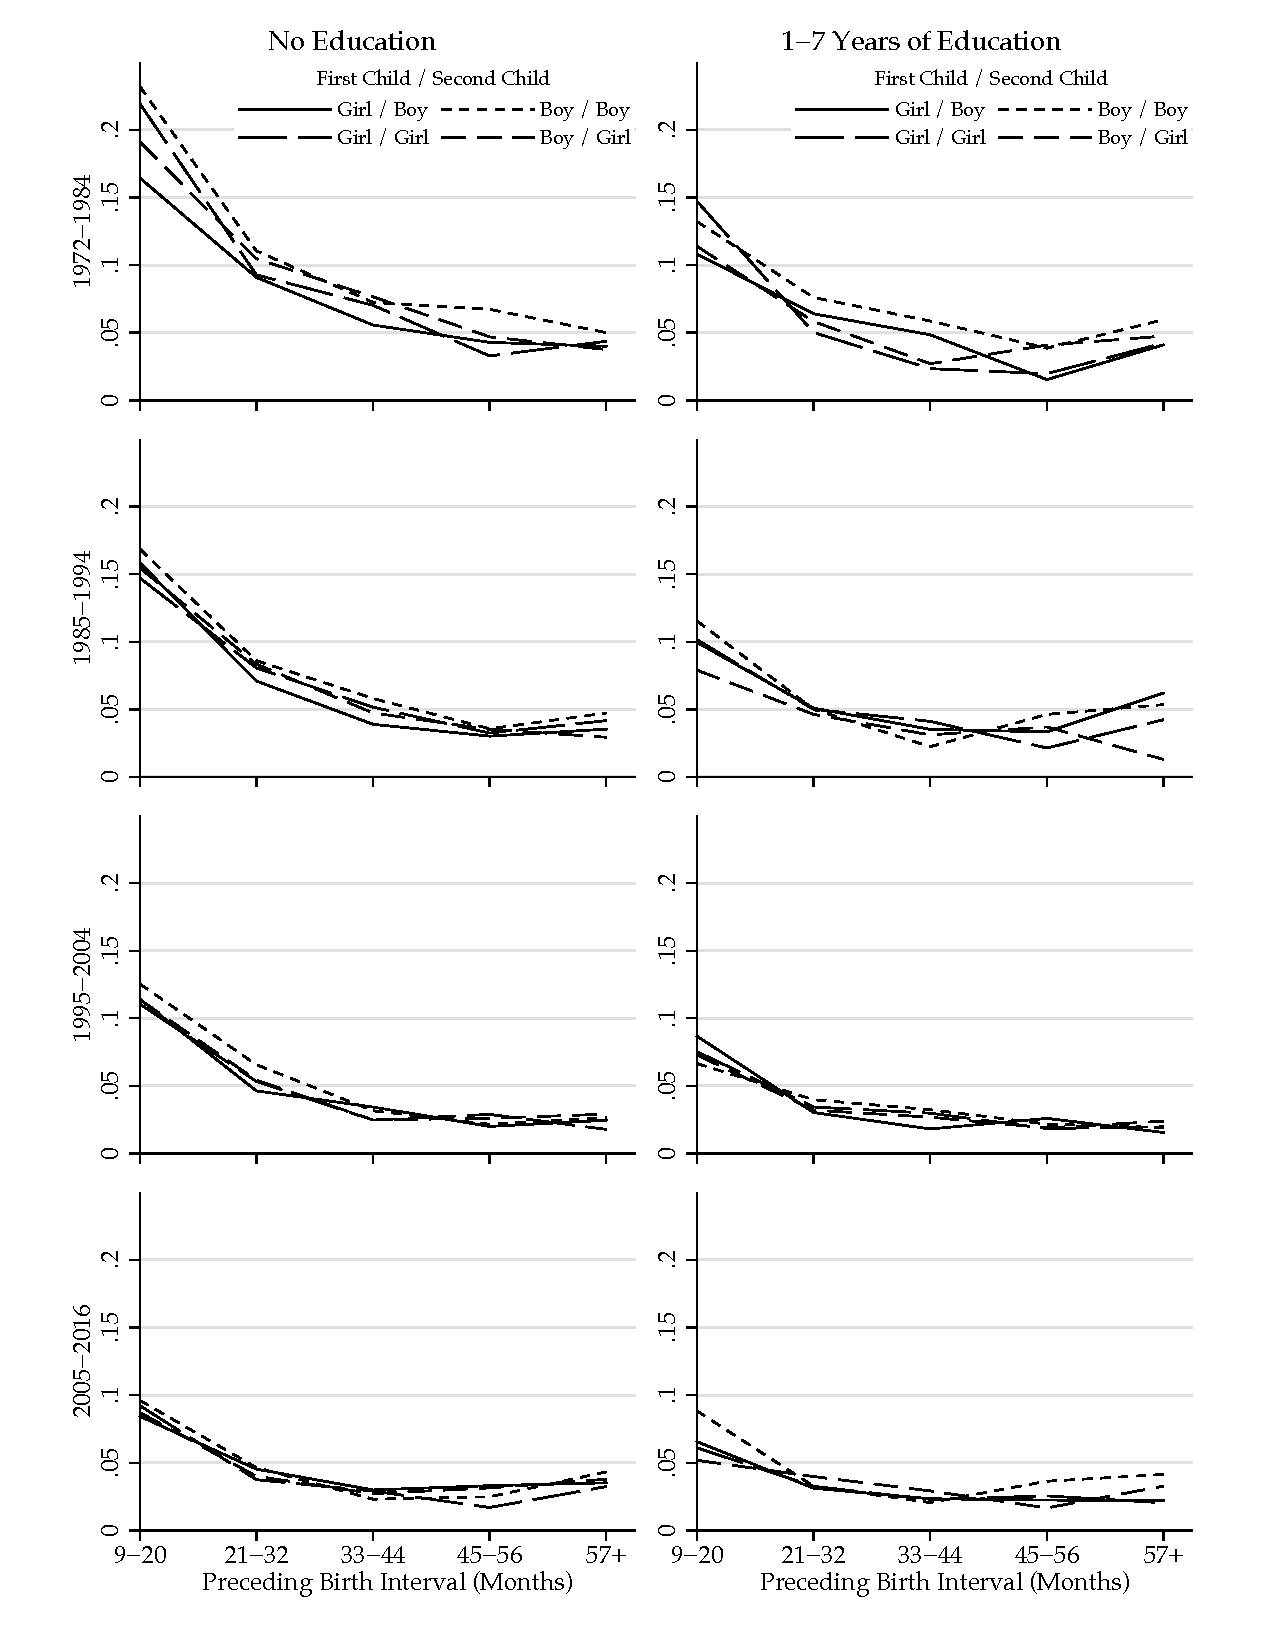
\includegraphics[width=\textwidth,height=\textheight,keepaspectratio=true]{mortality_spell_2_low_med}
\caption{Infant mortality by preceding birth interval across periods for second child of women with 
no education and women with 1--7 years of education}
\label{fig:mortality_low_med}
\end{figure}


\begin{figure}
\centering
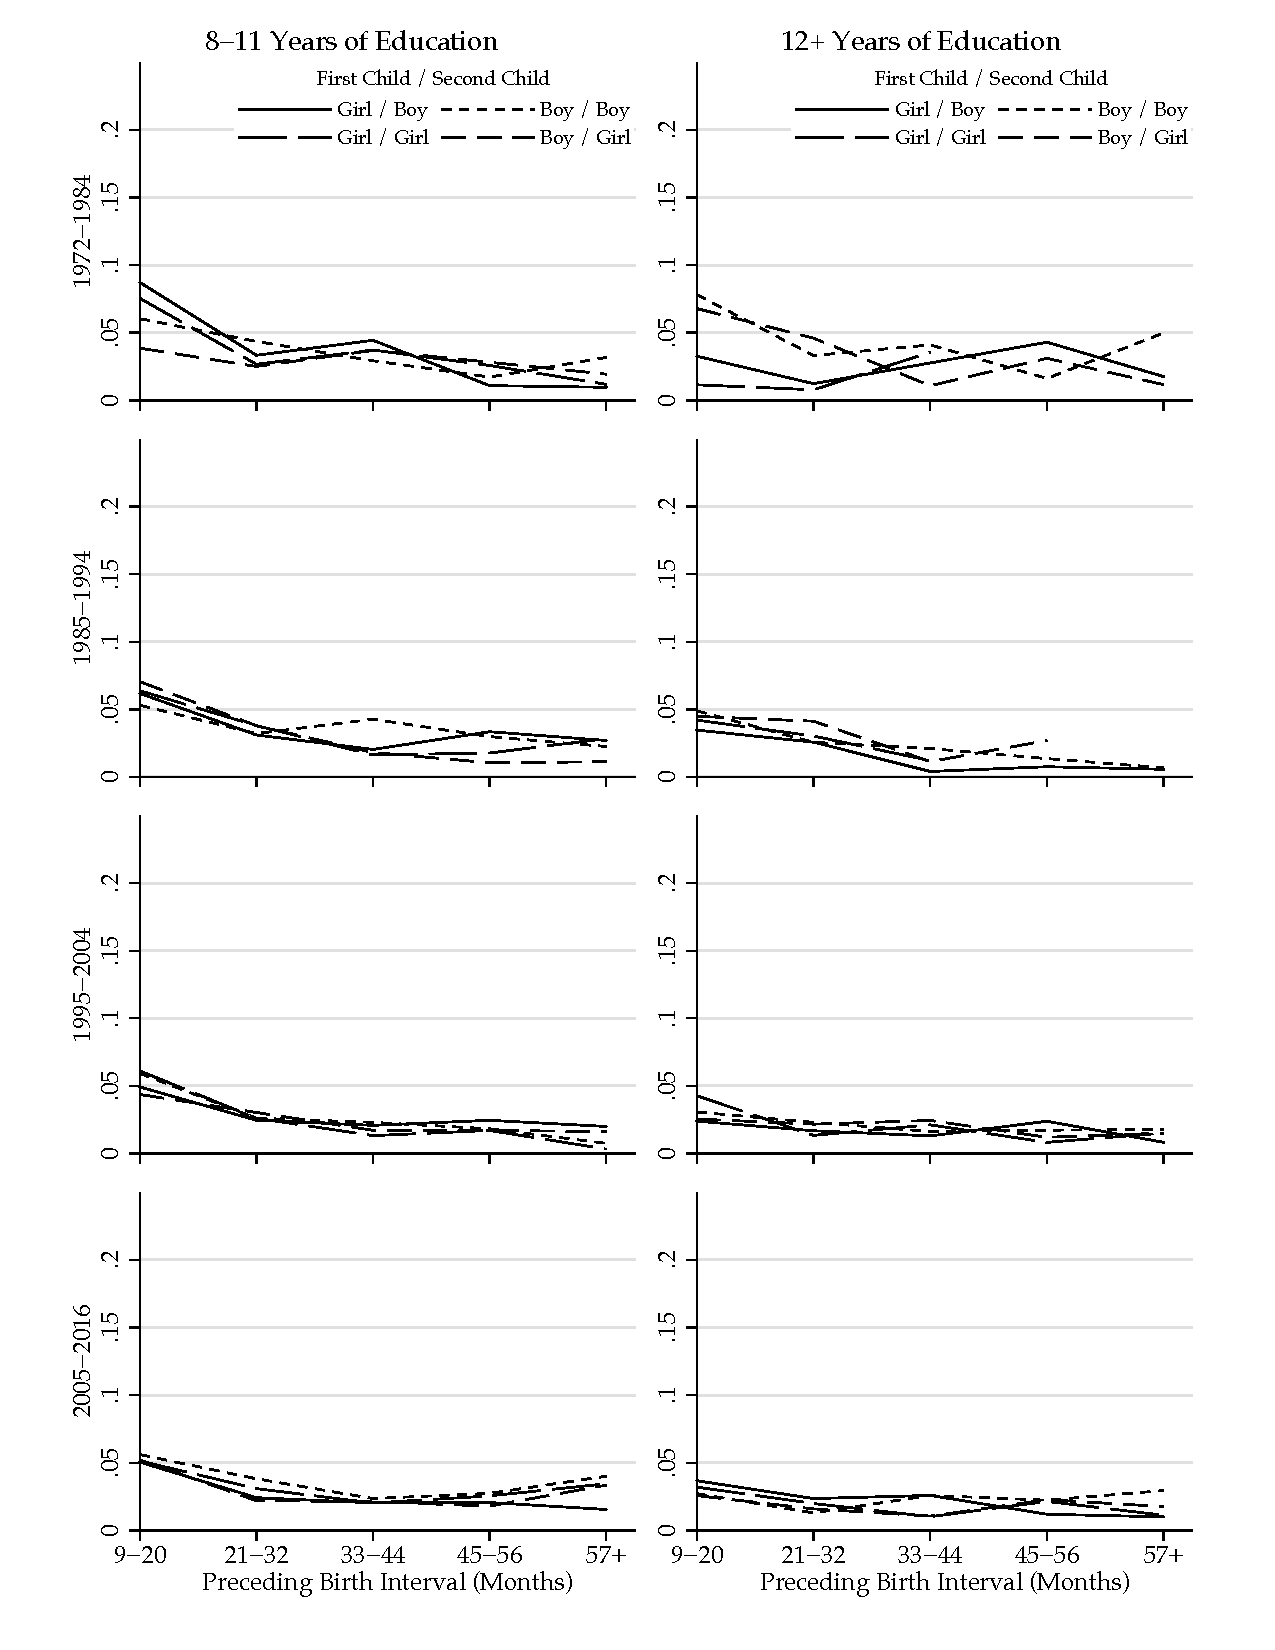
\includegraphics[width=\textwidth,height=\textheight,keepaspectratio=true]{mortality_spell_2_high_highest}
\caption{Infant mortality by preceding birth interval across periods for second child of women with 
8--11 and 12 and above years of education}
\label{fig:mortality_high_highest}
\end{figure}



There has been substantial convergence in mortality risk across groups over time.
For intervals 21 months or longer, there is now little difference across 
the education groups, with even the no-education group showing an infant mortality risk 
below 5\%.

Very short birth intervals still exhibit a higher mortality risk, although the 
effect declines with education level.
For the best-educated women, the mortality risk is 3\%--4\%,
whereas women with no education still show a risk that is close to 10\%.

Despite the prior findings of differential mortality by sex, there is little evidence 
that girls have substantially higher mortality risk.
There is some weak evidence that a boy born after a girl has a lower mortality
risk in the earliest periods.
However, this difference disappears with the general decline in mortality risk. 

Despite the concern that multiple abortions might increase mortality risk by shortening 
the interval between pregnancies, there is no evidence for this effect. 
Suppose sex-selective abortions lead to higher mortality risk. In that case, boys born 
after a girl---the solid lines---should have an increased risk with longer spacing for 
the two highest education groups in the last two periods.
However, there are no apparent consistent differences between these groups and the other 
potential combinations. 
The same holds for the third spell.

% line 3661 in an_infant_mortality.log
The raw numbers for women with the most uneven sex ratio also suggest that even with 
very high use of sex selection, there is no impact on mortality. 
A total of 1,004 women with 12 or more years of education and no boys at the start of 
the third spell in the last period had a third child, of which 685 were boys. 
Of these 685 boys, only six died within the first year of life. 
Half of those who died were born in the 9--32-month interval, and none in the 57-month+ 
interval.



\section{Conclusion\label{sec:conclusion}}

% Background
Over the past four decades, India saw a dramatic increase in the male-to-female
sex ratio at birth as access to sex selection spread and son preference remained high. 
Simultaneously, economic growth was strong, schooling increased, and the total
fertility rate fell to close to the replacement level.

% Questions
The main question I address in this paper is how birth spacing responded to the 
significant changes in India between 1972 and 2016, particularly the spread of sex 
selection.
I also examine two related questions.
First, did the changes in birth spacing bias the standard fertility estimates for India? 
Second, what is the relationship between infant mortality and the changes in birth spacing 
and sex selection?


% What has happened to spacing and why
The most substantial lengthening of birth intervals came from the best-educated women
because of their substantial use of sex selection combined with falling fertility.
Take, for example, women with 12 or more years of education who had two girls. 
As the sex ratio increased to close to 80\% boys, the expected median birth interval 
increased by almost 15 months, and the 75th percentile interval increased by 21 months.
Most of the increase in the long intervals came immediately after the introduction of sex 
selection in India.

Some of these increases are so large that we even observed a reversal of the traditional 
spacing pattern for some groups; when there are no sons, we now see the longest, rather 
than the shortest, birth intervals because of sex selection.
The women who are the least likely to use sex selection still show the traditional 
spacing pattern with short spacing in the absence of sons.

Son preference continues to show in fertility decisions. 
Fertility has declined for all groups, but the likelihood of having an additional child
still depends strongly on the number of sons, with women with no sons having the highest 
parity progression probabilities.

Birth intervals also lengthened in cases when sex selection is less likely to be used. 
However, compared to other countries with similar declines in fertility, the median 
spacing increases were smaller at three to six months over the period. 
Most of the median intervals when sex selection is less used are still short at 36 months 
or below. 
Furthermore, many women still have very short birth intervals. 
In many cases, more than 25\% have their next child within 24 months of the previous 
birth.  

% [predictions of declining sex selection] 
Despite predictions that the use of sex selection would decline, there is no clear 
evidence of this. 
The original users of sex selection continue to show substantial male-biased sex ratios, 
although there may be some leveling off. 
More concerning, sex selection appears to be spreading to less educated women as their 
fertility is falling.



% fertility bias

The increases in spacing make the total fertility rate a more biased measure of cohort 
fertility. 
This bias was most prominent early in the spread of sex selection when the fertility rate 
was up to one child lower than the predicted cohort fertility. 
However, it is still present, with the predicted cohort fertility 10\%--20\% 
higher than the fertility rate. 
At 1.8 children, the best-educated urban women are the only group for whom the predicted 
cohort fertility is below replacement.

Tempo effects are studied extensively in the literature \citep[see, for example, ][]{Bongaarts1999}.
Still, there are, to my knowledge, no other cases where there has been as 
substantial an increase in birth intervals and associated bias in fertility rates 
as for India.
It is conceivable that we might see increases in the total fertility rate as birth spacing 
stabilizes or even shortens again if interventions against sex selection are successful.


% Mortality
There has been a substantial reduction in infant mortality over time, and the size of the 
reductions is inversely related to the mother's education.
Hence, there is now little difference in mortality risk across education groups if the 
birth took place more than 21 months from the prior birth.
Short birth spacing is still associated with higher mortality, although the effect is 
small for the best-educated women.
There is no evidence that repeated abortions are associated with higher infant mortality 
for the child eventually born. 


% Implications 
The results here paint a less rosy picture of India's prospects for a continued reduction 
in population growth than generally accepted. 
With predicted cohort fertility still substantially higher than the fertility rate, 
India's total fertility rate will likely stabilize or even increase as birth intervals slow 
their lengthening. 
The more successful the attempts at combatting sex selection are, the more likely an 
increase in the total fertility rate will be. 
Furthermore, the rapid decline in infant mortality risk, combined with likely future 
declines as the proportion of very short birth intervals falls, may also slow the 
reduction in population growth. 



% Future research and policy 

There are two critical questions that future research should address.
First, sex selection means that girls-only families are less likely to have
very short birth intervals, which may reduce sibling competition. 
Hence, better health outcomes for girls with sex selection could be an unintended 
side-effect, rather than the result of girls becoming more valued as is often 
assumed \citep{Hu2015}. 
Comparing prior children's outcomes across sex composition and the sex of the next child 
could be a way to understand why girls' health outcomes improve in the presence of sex selection.

Second, what is the relationship between female labor force participation and sex selection? 
Women may be staying out of the labor market precisely because sex selection makes 
them more likely to have a boy and increases the expected birth spacing. 
Better job opportunities for women would affect sex selection for two reasons. 
First, it makes it more expensive to be out of the labor market for long periods. 
Second, it would moderate the differential in potential earnings between husband and wife 
and make it more attractive to invest in daughters' human capital. 
This approach could, however, be a double-edged sword. 
If better job opportunities further lower fertility, the use of sex selection may increase, 
everything else being equal.
Understanding the trade-off between long-term benefits from improvements in women's labor 
force participation and short-term costs from potential increases in sex selection is of 
paramount importance.


% The higher return to male offspring's human capital combined with access to sex
% selection may also explain another puzzle, why is the labor force participation so
% low when fertility is low and education has increased.
% As shown here, part of the answer may be that the number of children is, in fact, not as 
% low as previously thought, both because of the increased spacing and that more 
% children survive.



\clearpage

\onehalfspacing
\bibliographystyle{aer}
\bibliography{sex_selection_spacing}

\addcontentsline{toc}{section}{References}



\clearpage
\newpage

\appendix

% CHANGING NUMBERING OF FIGURES AND TABLES FOR APPENDIX
\renewcommand\thefigure{\thesection.\arabic{figure}}    
\renewcommand\thetable{\thesection.\arabic{table}}    

\section*{Appendices for Online Publication}

These appendices are intended for online publication.
They provide the descriptive statistics, additional
estimated duration tables, and graphs for all 
education groups and spells.

\clearpage
\newpage

\section{Characteristics of Women's Work Experiences}


\setcounter{figure}{0}
\setcounter{table}{0}

Figure \ref{fig:work_by_survey} shows the percent of married women who are 
currently working at the time of the survey by age group and education level.
No other labor force participation question is consistently available across all 
four surveys. 
Because the question refers to currently working, the percentages are lower in previous
studies. 

\captionsetup[figure]{skip = 10pt}

\begin{figure}[!htpb]
\centering
\rotatebox[origin=c]{90}{\small{40 Years or Older}}
\subfloat[Rural]{
    \begin{minipage}{0.45\textwidth}
        \includegraphics[width=\textwidth]{currently_working_rural_40}
    \end{minipage}
} 
\subfloat[Urban]{
    \begin{minipage}{0.45\textwidth}
        \includegraphics[width=\textwidth]{currently_working_urban_40} 
    \end{minipage}
}
\\
\rotatebox[origin=c]{90}{\small{30--39 Years Old}}
\subfloat[Rural]{
    \begin{minipage}{0.45\textwidth}
        \includegraphics[width=\textwidth]{currently_working_rural_30}
    \end{minipage}
} 
\subfloat[Urban]{
    \begin{minipage}{0.45\textwidth}
        \includegraphics[width=\textwidth]{currently_working_urban_30} 
    \end{minipage}
}
\\
\rotatebox[origin=c]{90}{\small{20--29 Years Old}}
\subfloat[Rural]{
    \begin{minipage}{0.45\textwidth}
        \includegraphics[width=\textwidth]{currently_working_rural_20}
    \end{minipage}
} 
\subfloat[Urban]{
    \begin{minipage}{0.45\textwidth}
        \includegraphics[width=\textwidth]{currently_working_urban_20} 
    \end{minipage}
}
\caption{Percentage of married women who were working at the time of the 
survey by age group and area of residence}
\label{fig:work_by_survey}
\end{figure}


\begin{figure}[!htpb]
\centering
\rotatebox[origin=c]{90}{\small{40 Years or Older}}
\subfloat[Rural]{
    \begin{minipage}{0.45\textwidth}
        \includegraphics[width=\textwidth]{work_cash_rural_40}
    \end{minipage}
} 
\subfloat[Urban]{
    \begin{minipage}{0.45\textwidth}
        \includegraphics[width=\textwidth]{work_cash_urban_40} 
    \end{minipage}
}
\\
\rotatebox[origin=c]{90}{\small{30--39 Years Old}}
\subfloat[Rural]{
    \begin{minipage}{0.45\textwidth}
        \includegraphics[width=\textwidth]{work_cash_rural_30}
    \end{minipage}
} 
\subfloat[Urban]{
    \begin{minipage}{0.45\textwidth}
        \includegraphics[width=\textwidth]{work_cash_urban_30} 
    \end{minipage}
}
\\
\rotatebox[origin=c]{90}{\small{20--29 Years Old}}
\subfloat[Rural]{
    \begin{minipage}{0.45\textwidth}
        \includegraphics[width=\textwidth]{work_cash_rural_20}
    \end{minipage}
} 
\subfloat[Urban]{
    \begin{minipage}{0.45\textwidth}
        \includegraphics[width=\textwidth]{work_cash_urban_20} 
    \end{minipage}
}
\caption{Percentage of women paid cash or cash and in-kind of those women who were 
working at the time of the survey by age group and area of residence}
\label{fig:work_cash_by_survey}
\end{figure}



\begin{figure}[!htpb]
\centering
\rotatebox[origin=c]{90}{\small{40 Years or Older}}
\subfloat[Rural]{
    \begin{minipage}{0.45\textwidth}
        \includegraphics[width=\textwidth]{work_family_rural_40}
    \end{minipage}
} 
\subfloat[Urban]{
    \begin{minipage}{0.45\textwidth}
        \includegraphics[width=\textwidth]{work_family_urban_40} 
    \end{minipage}
}
\\
\rotatebox[origin=c]{90}{\small{30--39 Years Old}}
\subfloat[Rural]{
    \begin{minipage}{0.45\textwidth}
        \includegraphics[width=\textwidth]{work_family_rural_30}
    \end{minipage}
} 
\subfloat[Urban]{
    \begin{minipage}{0.45\textwidth}
        \includegraphics[width=\textwidth]{work_family_urban_30} 
    \end{minipage}
}
\\
\rotatebox[origin=c]{90}{\small{20--29 Years Old}}
\subfloat[Rural]{
    \begin{minipage}{0.45\textwidth}
        \includegraphics[width=\textwidth]{work_family_rural_20}
    \end{minipage}
} 
\subfloat[Urban]{
    \begin{minipage}{0.45\textwidth}
        \includegraphics[width=\textwidth]{work_family_urban_20} 
    \end{minipage}
}
\caption{Percentage women who worked for a family member of those 
working at the time of the survey, by age group and area of residence}
\label{fig:work_family_by_survey}
\end{figure}


\clearpage
\newpage

\section{Empirical Model Details}

\setcounter{figure}{0}
\setcounter{table}{0}

% [More formal version of empirical strategy section]


The model is a discrete time, nonproportional, competing risk hazard model with two exit 
states: Either a boy or a girl is born.
The unit of analysis is a spell, the period from nine months after one birth to the next.
For each woman, $i=1,\ldots,n$, the starting point for a spell is time $t=1$, and 
the spell continues until time $t_i$, when either a birth occurs or the spell 
is censored.%
\footnote{
The time of censoring is assumed independent of the hazard rate,
as is standard in the literature.
}
There are two exit states: The birth of a boy, $j=1$, or the birth of a girl, $j=2$, and 
$J_i$ is a random variable indicating which event took place.
The discrete time hazard rate $h_{ijt}$ is 
\begin{equation}
 h_{ijt} = \frac{\exp(D_j(t) + \alpha_{jt}'\mathbf{Z}_{it} + \beta_j'\mathbf{X}_{i})} 
 {1 + \sum_{l=1}^2 \exp(D_j(t) + \alpha_{lt}'\mathbf{Z}_{it} + \beta_l'\mathbf{X}_{i})} \: \: \; \; \;  j = 1,2
 \label{eq:hazard_appendix}
\end{equation}
where the explanatory variable vectors, $\mathbf{Z}_{it}$ and $\mathbf{X}_{i}$, capture 
individual, household, and community characteristics,
and $D_{j}(t)$ is the piece-wise linear baseline hazard for outcome $j$, captured
by dummies and the associated coefficients,
\begin{equation}
D_j(t) = \gamma_{j1} D_1 + \gamma_{j2} D_2 + \ldots + \gamma_{jT} D_T,
\end{equation}
with $D_m = 1$ if $t=m$ and zero otherwise.
This approach to modeling the baseline hazard is flexible and does not place 
overly strong restrictions on the baseline hazard.

The explanatory variables in $\mathbf{Z}$, and the interactions between them, 
constitute the nonproportional part of the model, which means that they are
interacted with the baseline hazard:
\begin{equation}
 \mathbf{Z}_{it} = D_j(t) \times (\mathbf{Z}_1 + Z_2 + \mathbf{Z}_1 \times Z_2),
\end{equation}
where $D_j(t)$ is the piece-wise linear baseline hazard, $\mathbf{Z}_1$ captures sex 
composition of previous children, if any, and $Z_2$ captures area of residence.
The remaining explanatory variables, $\mathbf{X}$, enter proportionally,
but to further minimize any potential bias from assuming proportionality, estimations 
are done separately for different levels of mothers' education and different 
periods.

Equation (\ref{eq:hazard_appendix}) is equivalent to the logistic hazard model and has the same 
likelihood function as the multinomial logit model \citep{allison82,jenkins95}.
Hence, transforming the data, so each observation is an interval---here equal
to three months---the model can be estimated using a standard multinomial logit model.

The distribution of spacing is captured by the survival curve, which shows the probability 
of not having had a birth yet by spell duration, for a given set of explanatory variables.
The survival curve at time $t$ is 
\begin{equation}
\label{eq:survival}
S_{t} 
= 
\prod_{d=1}^t
\left(
\frac{ 1 }
{1 + \sum_{l=2}^2 \exp(D_j(t) + \alpha_{ld}'\mathbf{Z}_{kd} + \beta_l'\mathbf{X}_{k})}
\right).
\end{equation}

% Because the probability of ever having a next birth varies across groups, a direct 
% comparison of standard survival curves tells us little about how the spread of sex 
% selection affects birth spacing across groups.
% I, therefore, condition on the predicted likelihood of parity progression when examining 
% birth spacing measures, such as the average duration to a birth.
% The reliability of this approach depends on whether the spell length covered is 
% sufficiently long that few women are likely to give birth after the spell cut-off.
% I discuss the choice of spell length below.%
% \footnote{
% It is important to note that the approach is not the same as merely calculating 
% the birth spacing measures for women who already have a given 
% parity child in the survey because that number does not take into account
% the censoring of spells that will eventually lead to a birth.
% }
% In addition, I present graphs of survival curves conditional on parity progression,
% which therefore begin at 100\% and end at 0\%.

Interpretation of the model coefficients is challenging \citep{thomas96}.
It is, however, possible to calculate the predicted probabilities of 
having a boy, $b$, and of having a girl, $g$, in period $t$, conditional on 
a set of explanatory variables and not having had a child before that period, as
\begin{align}
P(b_{t} | \mathbf{X}_{k}, \mathbf{Z}_{kt}, t ) 
& =  
\frac{ \exp(D_j(t) + \alpha_{1t}' \mathbf{Z}_{kt} + \beta_1' \mathbf{X}_{k} )}
{1 + \sum_{l=1}^2 \exp(D_j(t) + \alpha_{lt} ' \mathbf{Z}_{kt} + \beta_l ' \mathbf{X}_{k})}
\label{eq:probability_boy} \\
P(g_{t} | \mathbf{X}_{k}, \mathbf{Z}_{kt},t ) 
& =  
\frac{ \exp(D_j(t) + \alpha_{2t}'\mathbf{Z}_{kt} + \beta_2'\mathbf{X}_{k} )}
{1 + \sum_{l=2}^2 \exp(D_j(t) + \alpha_{lt}'\mathbf{Z}_{kt} + \beta_l'\mathbf{X}_{k})}
\label{eq:probability_girl}
\end{align}
It is then straightforward to calculate the estimated percentage of children born that 
are boys, $\hat{Y}$, at each $t$:  
\begin{equation}
\hat{Y}_t 
= 
\frac{ P(b_{t} | \mathbf{X}_{k}, \mathbf{Z}_{kt},t )}
{ P(b_{t} | \mathbf{X}_{k}, \mathbf{Z}_{kt},t) + P(g_{t} | \mathbf{X}_{k}, \mathbf{Z}_{kt},t )} 
\times 100.
\label{eq:probability_son}
\end{equation}
Combining the percentage boys and the likelihood of exiting the spell 
across all $t$ gives the predicted percent boys born over the entire spell.%
\footnote{
Imagine $T=2$. 
If 54\% and 66\% of births are boys and the likelihood of giving birth 20\% and 40\%, 
then the predicted sex ratio is $\frac{54*0.2+66*0.4}{0.2+0.4} = 62$\% boys. 
}




\clearpage
\newpage

\section{Recall Error and the Sex Ratio}

\setcounter{figure}{0}
\setcounter{table}{0}

The reliability of the results depends on the correctness of the birth histories
provided by the respondents.
A significant concern here is underreporting of child mortality, especially a systematic
recall error where respondents' likelihood of reporting a deceased child depends on the 
sex of that child. 
This appendix section assesses the degree of recall error across the surveys and discusses 
methods to address it.

NFHS enumerators probe for any missed births, although the method depends on the survey.
NFHS-1 probe for each calendar birth interval that is four or more years.
NFHS-2 asked for stillbirths, spontaneous and induced abortions and also probed 
for each calendar birth interval four or more years.
NFHS-3 and NFHS-4 did not directly use birth intervals, but asked whether there were any 
other live births between (name of previous birth) and (name), including any children who 
died after birth, and asked for births before the birth listed as first birth and
after the last birth listed as the last birth.

Probing catches many initially missed births, but systematic recall error based on son
preference may still be a problem.
First, son preference leads to significantly higher mortality for girls than boys.
Secondly, son preference makes it more likely that parents will remember deceased boys 
than deceased girls.
Finally, in the absence of sex-selective abortions, parents with a preference for sons may
have the next birth sooner if the last child was a girl than if it was a boy.
If this girl subsequently dies, she is more likely to be missed if probing for missed 
births is only done for long intervals as in NFHS-1 and NFHS-2.

I use two approaches to examine the degree of recall error.
The first approach is to test whether the observed sex ratio is significantly different
from the natural sex ratio.
The natural sex ratio is approximately 105 boys to 100 girls or
51.2\% \citep{ben-porath76b,jacobsen99,Portner2015b}.
Prenatal sex determination techniques did not become widely available until the mid-1980s, 
so any significant deviation from the natural sex ratio before that time is likely the 
result of recall error.
The second approach is to compare births that took place during the same period but
where captured in different surveys.
Recall error is likely to increase with time, so births and deaths that took place earlier 
are more likely to be subject to recall error than more recent events.

Table \ref{tab:recallBirthBO1} shows the sex ratios of children recorded as first-born by 
year of birth, together with tests for whether the observed sex ratio is significantly 
higher than the natural sex ratio and whether more recent surveys have a higher sex ratio 
for the cohort than earlier surveys for the same period births.
Births are combined into five-year cohorts to achieve sufficient power.

\input{../tables/recallBirthBO1.tex}

% \input{../tables/recallBirthBO2.tex}


The ``first-born'' sex ratios illustrate the systematic recall error problem well.
In all four surveys around 55\% of children reported as first-born are boys
for the first cohort of births observed.
Given that these cohorts cover from 1960-1964 to 1980-1984, which is before sex selection 
techniques became available in India, the most likely explanation for the skewed sex ratio 
is that some children listed as first-borns were not, in fact, the first children born in 
their families.
Instead, for a substantial proportion of families, their first-born was a girl who died 
and went unreported when enumerators asked about birth history.

As expected, the difference between the observed sex ratio and the natural sex ratio is 
less pronounced the closer to the survey date the cohort is.
The observed sex ratio for children born just before the NFHS-1 survey and listed as 
first-born is 0.517, which is not statistically significantly different from the
natural sex ratio.
The same general pattern holds for the other three surveys, with cohorts further away
from the survey date more likely to have a sex ratio skewed male.

% Second births show a pattern very similar to that for first births.
% An interesting difference is that there is evidence of a U-shaped relationship between
% time and sex ratio for second births.
% Cohorts furthest away from the survey year show the highest sex ratios, but declines to the
% natural sex ratio in the mid-1980s, and the sex ratio is then significantly higher again 
% for more recent births.
% This is in line with the results in the main paper that show that sex selective abortions 
% take place on lower parity births as desired fertility declined.

Finally, across surveys, the same cohort tends to show a higher sex ratio the more recent 
the survey (births in the cohort took place earlier relative to the survey date).
Despite this, few cohorts show significantly different sex ratios across surveys, most 
likely because of a lack of power.
The exception is that comparisons involving NFHS-4 are mostly statistically significant
since the number of surveyed households in NFHS-4 were much larger than in prior surveys.

The problem with the above approach is that the year of birth is affected by recall error; 
a second born child listed as first-born is born later than the real first born child.
Year of marriage should, however, be affected neither by parental recall error 
nor the use of sex-selective abortions.
Tables \ref{tab:recallMarriageBO1} and \ref{tab:recallMarriageBO2}, therefore, shows sex 
ratios of children recorded as first-born and second-born by year of parents' marriage, 
together with tests for whether the observed sex ratio is significantly higher than the 
natural sex ratio and whether more recent surveys show a higher sex ratio for the cohort 
than earlier surveys.
The basic recall error pattern remains, with women married longer ago more
likely to report that their first-born is a boy.
Similarly, comparing women married in the same five-year period across surveys shows
that women married longer ago are more likely to report having a son.


\input{../tables/recallMarriageBO1.tex}

\input{../tables/recallMarriageBO2.tex}


The relationship between the length of marriage and recall error can also be seen in 
Figures \ref{fig:sex_ratio_recall_rounds_bo1} and \ref{fig:sex_ratio_recall_rounds_bo2}, 
which show the observed sex ratio for children reported as first born as a function of 
the duration of marriage at the time of the survey.
The solid line is the sex ratio of children reported as first-born by the number of years 
between the survey and marriage, while the dashed lines indicate the 95\% confidence 
interval and the horizontal line the natural sex ratio (approximately 0.512).
To ensure sufficient cell sizes I group years into twos.
In line with the results from Tables \ref{tab:recallMarriageBO1} and 
\ref{tab:recallMarriageBO2}, the observed ratio of boys is increasingly above the expected 
value the longer ago the parents were married.

\begin{figure}
\centering
\subfloat[NFHS-1]{\includegraphics[width=.49\textwidth]{recall_sex_ratio_marriage_round_1}}
\subfloat[NFHS-2]{\includegraphics[width=.49\textwidth]{recall_sex_ratio_marriage_round_2}} \\
\subfloat[NFHS-3]{\includegraphics[width=.49\textwidth]{recall_sex_ratio_marriage_round_3}} 
\subfloat[NFHS-4]{\includegraphics[width=.49\textwidth]{recall_sex_ratio_marriage_round_4}} 
\caption{Ratio of Boys for ``First'' Births by Survey Round}
\label{fig:sex_ratio_recall_rounds_bo1}
\end{figure}

\begin{figure}
\centering
\subfloat[NFHS-1]{\includegraphics[width=.49\textwidth]{recall_sex_ratio_marriage_round_1_bo2}}
\subfloat[NFHS-2]{\includegraphics[width=.49\textwidth]{recall_sex_ratio_marriage_round_2_bo2}} \\
\subfloat[NFHS-3]{\includegraphics[width=.49\textwidth]{recall_sex_ratio_marriage_round_3_bo2}} 
\subfloat[NFHS-4]{\includegraphics[width=.49\textwidth]{recall_sex_ratio_marriage_round_4_bo2}} 
\caption{Ratio of Boys for ``Second'' Births by Survey Round}
\label{fig:sex_ratio_recall_rounds_bo2}
\end{figure}


The increasingly unequal sex ratio with increasing marriage duration suggests that
a solution to the recall error problem is to drop observations for 
women who were married ``too far'' from the survey year.
The main problem is establishing what the best cut-off point should be, with the
trade-off between retaining enough observations and the correctness of the information.
As Tables \ref{tab:recallMarriageBO1} and \ref{tab:recallMarriageBO2} show, there are 
differences in recall error across the three surveys and between the two birth
orders, although this may be the result of differences in the number of observations 
across surveys.
Furthermore, the recall error pattern is not entirely consistent across observed birth 
orders.
Since most of the surveys start showing significantly biased sex ratio from around 22
years of marriage on, I drop all observations where the marriage took place 22 years
or more.


\clearpage
\newpage

\section{Descriptive Statistics}
\setcounter{figure}{0}
\setcounter{table}{0}


% Descriptive statistics tables
\input{../tables/des_stat.tex}

\clearpage
\newpage



\section{Additional Results Figures and  Tables}

\setcounter{figure}{0}
\setcounter{table}{0}

\captionsetup[figure]{skip = -16pt}

Figures \ref{fig:spacing_low_urban} and \ref{fig:spacing_highest_rural} show 25th, 50th,
and 75th percentile birth intervals, the sex ratio, and the probability of parity
progression by spell for urban women with no education and rural women with 12 or
more years of education, respectively.

\begin{figure}
\centering
\includegraphics[width=\textwidth,height=\textheight,keepaspectratio=true]{bs_low_urban}
\caption{Percentile birth intervals, sex ratios, and parity progression  
for urban women with no education by spell, sex composition, and period}
\label{fig:spacing_low_urban}
\end{figure}

\begin{figure}
\centering
\includegraphics[width=\textwidth,height=\textheight,keepaspectratio=true]{bs_highest_rural}
\caption{Percentile birth intervals, sex ratios, and parity progression  
for rural women with 12 or more years of education by spell, sex composition, and period}
\label{fig:spacing_highest_rural}
\end{figure}



The first set of tables, Tables \ref{tab:p25_p50_p75_low}, \ref{tab:p25_p50_p75_med},
\ref{tab:p25_p50_p75_high}, and \ref{tab:p25_p50_p75_highest} show 25th, 50th, and
75th percentile birth intervals together with their standard errors.
The standard errors for all measures are based on bootstrapping,
where the model is repeatedly estimated using resampling with replacement.

The second set of tables, 
Tables \ref{tab:avg_sex_ratio_low}, \ref{tab:avg_sex_ratio_med}, 
\ref{tab:avg_sex_ratio_high}, and \ref{tab:avg_sex_ratio_highest}, show predicted average 
birth intervals, sex ratios, and probabilities of having a birth by decade, spell, and sex 
composition for the four education levels separated by the area of residence, together 
with bootstrapped standard errors for all three outcomes.
To find the average birth interval, I calculate, for each woman, the probability of 
giving birth in each $t$, and her expected spell length from these probabilities. 
I then average the individual expected spell lengths across women using their parity 
progression probabilities as weights. Finally, I add nine months because spells begin 
nine months after the previous birth.

I also show whether durations for sex composition other than only girls are statistically 
significantly different from the duration with only girls based on bootstrapped 
differences. 
The cleanest test is comparing durations after only boys with durations after
only girls, but the number of births to women with only sons becomes small 
in the later periods.
Hence, it is possible to have substantial differences in spacing that are
not statistically significant because of low power, especially for the third 
and fourth spell.

Each predicted percent of boys is tested against the natural percentage of
boys using the bootstrapped standard errors.
The natural sex ratio is approximately 105 boys to 100 girls or
51.2\% \citep{ben-porath76b,jacobsen99,Portner2015b}.
The predicted percentage boys may differ from the natural rate because of 
natural variation, any remaining recall error not corrected for, or 
sex selection. 

\input{../tables/bootstrap_duration_p25_p75_low_all.tex}

\input{../tables/bootstrap_duration_p25_p75_med_all.tex}

\input{../tables/bootstrap_duration_p25_p75_high_all.tex}

\input{../tables/bootstrap_duration_p25_p75_highest_all.tex}

\input{../tables/bootstrap_duration_avg_sex_ratio_low_all.tex}

\input{../tables/bootstrap_duration_avg_sex_ratio_med_all.tex}

\input{../tables/bootstrap_duration_avg_sex_ratio_high_all.tex}

\input{../tables/bootstrap_duration_avg_sex_ratio_highest_all.tex}



\clearpage

% \begin{figure}[htpb]
% \captionsetup[subfigure]{labelformat=empty,position=top}
% \captionsetup{font=footnotesize,skip=2pt}
% \centering
% \caption*{No education}
% \subfloat[][Second Spell]{\includegraphics[width=0.32\textwidth]{p25_spell2_low_urban}}
% \subfloat[][Third Spell]{\includegraphics[width=0.32\textwidth]{p25_spell3_low_urban}}
% \subfloat[][Fourth Spell]{\includegraphics[width=0.32\textwidth]{p25_spell4_low_urban}}
% \\
% \caption*{One to Seven Years of Education}
% \subfloat[][Second Spell]{\includegraphics[width=0.32\textwidth]{p25_spell2_med_urban}}
% \subfloat[][Third Spell]{\includegraphics[width=0.32\textwidth]{p25_spell3_med_urban}}
% \subfloat[][Fourth Spell]{\includegraphics[width=0.32\textwidth]{p25_spell4_med_urban}}
% \\
% \caption*{Eight to Eleven Years of Education}
% \subfloat[][Second Spell]{\includegraphics[width=0.32\textwidth]{p25_spell2_high_urban}}
% \subfloat[][Third Spell]{\includegraphics[width=0.32\textwidth]{p25_spell3_high_urban}}
% \subfloat[][Fourth Spell]{\includegraphics[width=0.32\textwidth]{p25_spell4_high_urban}}
% \\
% \caption*{Twelve or More Years of Education}
% \subfloat[][Second Spell]{\includegraphics[width=0.32\textwidth]{p25_spell2_highest_urban}}
% \subfloat[][Third Spell]{\includegraphics[width=0.32\textwidth]{p25_spell3_highest_urban}}
% \begin{minipage}{0.32\textwidth}\hspace{1cm}\end{minipage}
% \captionsetup{font=normalsize}
% \caption{
% Changes in 25th Percentile Birth Intervals for Urban Women by Spell and Education
% }
% \label{fig:p25_urban}
% \end{figure}
% 
% 
% \begin{figure}[htpb]
% \captionsetup[subfigure]{labelformat=empty,position=top}
% \captionsetup{font=footnotesize,skip=2pt}
% \centering
% \caption*{No education}
% \subfloat[][Second Spell]{\includegraphics[width=0.32\textwidth]{p25_spell2_low_rural}}
% \subfloat[][Third Spell]{\includegraphics[width=0.32\textwidth]{p25_spell3_low_rural}}
% \subfloat[][Fourth Spell]{\includegraphics[width=0.32\textwidth]{p25_spell4_low_rural}}
% \\
% \caption*{One to Seven Years of Education}
% \subfloat[][Second Spell]{\includegraphics[width=0.32\textwidth]{p25_spell2_med_rural}}
% \subfloat[][Third Spell]{\includegraphics[width=0.32\textwidth]{p25_spell3_med_rural}}
% \subfloat[][Fourth Spell]{\includegraphics[width=0.32\textwidth]{p25_spell4_med_rural}}
% \\
% \caption*{Eight to Eleven Years of Education}
% \subfloat[][Second Spell]{\includegraphics[width=0.32\textwidth]{p25_spell2_high_rural}}
% \subfloat[][Third Spell]{\includegraphics[width=0.32\textwidth]{p25_spell3_high_rural}}
% \subfloat[][Fourth Spell]{\includegraphics[width=0.32\textwidth]{p25_spell4_high_rural}}
% \\
% \caption*{Twelve or More Years of Education}
% \subfloat[][Second Spell]{\includegraphics[width=0.32\textwidth]{p25_spell2_highest_rural}}
% \subfloat[][Third Spell]{\includegraphics[width=0.32\textwidth]{p25_spell3_highest_rural}}
% \begin{minipage}{0.32\textwidth}\hspace{1cm}\end{minipage}
% \captionsetup{font=normalsize}
% \caption{
% Changes in 25th Percentile Birth Intervals for Rural Women by Spell and Education
% }
% \label{fig:p25_rural}
% \end{figure}
% 
% \begin{figure}[htpb]
% \captionsetup[subfigure]{labelformat=empty,position=top}
% \captionsetup{font=footnotesize,skip=2pt}
% \centering
% \caption*{No education}
% \subfloat[][Second Spell]{\includegraphics[width=0.32\textwidth]{p50_spell2_low_urban}}
% \subfloat[][Third Spell]{\includegraphics[width=0.32\textwidth]{p50_spell3_low_urban}}
% \subfloat[][Fourth Spell]{\includegraphics[width=0.32\textwidth]{p50_spell4_low_urban}}
% \\
% \caption*{One to Seven Years of Education}
% \subfloat[][Second Spell]{\includegraphics[width=0.32\textwidth]{p50_spell2_med_urban}}
% \subfloat[][Third Spell]{\includegraphics[width=0.32\textwidth]{p50_spell3_med_urban}}
% \subfloat[][Fourth Spell]{\includegraphics[width=0.32\textwidth]{p50_spell4_med_urban}}
% \\
% \caption*{Eight to Eleven Years of Education}
% \subfloat[][Second Spell]{\includegraphics[width=0.32\textwidth]{p50_spell2_high_urban}}
% \subfloat[][Third Spell]{\includegraphics[width=0.32\textwidth]{p50_spell3_high_urban}}
% \subfloat[][Fourth Spell]{\includegraphics[width=0.32\textwidth]{p50_spell4_high_urban}}
% \\
% \caption*{Twelve or More Years of Education}
% \subfloat[][Second Spell]{\includegraphics[width=0.32\textwidth]{p50_spell2_highest_urban}}
% \subfloat[][Third Spell]{\includegraphics[width=0.32\textwidth]{p50_spell3_highest_urban}}
% \begin{minipage}{0.32\textwidth}\hspace{1cm}\end{minipage}
% \captionsetup{font=normalsize}
% \caption{
% Changes in 50th Percentile Birth Intervals for Urban Women by Spell and Education
% }
% \label{fig:p50_urban}
% \end{figure}
% 
% 
% \begin{figure}[htpb]
% \captionsetup[subfigure]{labelformat=empty,position=top}
% \captionsetup{font=footnotesize,skip=2pt}
% \centering
% \caption*{No education}
% \subfloat[][Second Spell]{\includegraphics[width=0.32\textwidth]{p50_spell2_low_rural}}
% \subfloat[][Third Spell]{\includegraphics[width=0.32\textwidth]{p50_spell3_low_rural}}
% \subfloat[][Fourth Spell]{\includegraphics[width=0.32\textwidth]{p50_spell4_low_rural}}
% \\
% \caption*{One to Seven Years of Education}
% \subfloat[][Second Spell]{\includegraphics[width=0.32\textwidth]{p50_spell2_med_rural}}
% \subfloat[][Third Spell]{\includegraphics[width=0.32\textwidth]{p50_spell3_med_rural}}
% \subfloat[][Fourth Spell]{\includegraphics[width=0.32\textwidth]{p50_spell4_med_rural}}
% \\
% \caption*{Eight to Eleven Years of Education}
% \subfloat[][Second Spell]{\includegraphics[width=0.32\textwidth]{p50_spell2_high_rural}}
% \subfloat[][Third Spell]{\includegraphics[width=0.32\textwidth]{p50_spell3_high_rural}}
% \subfloat[][Fourth Spell]{\includegraphics[width=0.32\textwidth]{p50_spell4_high_rural}}
% \\
% \caption*{Twelve or More Years of Education}
% \subfloat[][Second Spell]{\includegraphics[width=0.32\textwidth]{p50_spell2_highest_rural}}
% \subfloat[][Third Spell]{\includegraphics[width=0.32\textwidth]{p50_spell3_highest_rural}}
% \begin{minipage}{0.32\textwidth}\hspace{1cm}\end{minipage}
% \captionsetup{font=normalsize}
% \caption{
% Changes in 50th Percentile Birth Intervals for Rural Women by Spell and Education
% }
% \label{fig:p50_rural}
% \end{figure}
% 
% 
% \begin{figure}[htpb]
% \captionsetup[subfigure]{labelformat=empty,position=top}
% \captionsetup{font=footnotesize,skip=2pt}
% \centering
% \caption*{No education}
% \subfloat[][Second Spell]{\includegraphics[width=0.32\textwidth]{avg_spell2_low_urban}}
% \subfloat[][Third Spell]{\includegraphics[width=0.32\textwidth]{avg_spell3_low_urban}}
% \subfloat[][Fourth Spell]{\includegraphics[width=0.32\textwidth]{avg_spell4_low_urban}}
% \\
% \caption*{One to Seven Years of Education}
% \subfloat[][Second Spell]{\includegraphics[width=0.32\textwidth]{avg_spell2_med_urban}}
% \subfloat[][Third Spell]{\includegraphics[width=0.32\textwidth]{avg_spell3_med_urban}}
% \subfloat[][Fourth Spell]{\includegraphics[width=0.32\textwidth]{avg_spell4_med_urban}}
% \\
% \caption*{Eight to Eleven Years of Education}
% \subfloat[][Second Spell]{\includegraphics[width=0.32\textwidth]{avg_spell2_high_urban}}
% \subfloat[][Third Spell]{\includegraphics[width=0.32\textwidth]{avg_spell3_high_urban}}
% \subfloat[][Fourth Spell]{\includegraphics[width=0.32\textwidth]{avg_spell4_high_urban}}
% \\
% \caption*{Twelve or More Years of Education}
% \subfloat[][Second Spell]{\includegraphics[width=0.32\textwidth]{avg_spell2_highest_urban}}
% \subfloat[][Third Spell]{\includegraphics[width=0.32\textwidth]{avg_spell3_highest_urban}}
% \begin{minipage}{0.32\textwidth}\hspace{1cm}\end{minipage}
% \captionsetup{font=normalsize}
% \caption{
% Changes in Average Birth Intervals for Urban Women by Spell and Education
% }
% \label{fig:avg_urban}
% \end{figure}
% 
% 
% \begin{figure}[htpb]
% \captionsetup[subfigure]{labelformat=empty,position=top}
% \captionsetup{font=footnotesize,skip=2pt}
% \centering
% \caption*{No education}
% \subfloat[][Second Spell]{\includegraphics[width=0.32\textwidth]{avg_spell2_low_rural}}
% \subfloat[][Third Spell]{\includegraphics[width=0.32\textwidth]{avg_spell3_low_rural}}
% \subfloat[][Fourth Spell]{\includegraphics[width=0.32\textwidth]{avg_spell4_low_rural}}
% \\
% \caption*{One to Seven Years of Education}
% \subfloat[][Second Spell]{\includegraphics[width=0.32\textwidth]{avg_spell2_med_rural}}
% \subfloat[][Third Spell]{\includegraphics[width=0.32\textwidth]{avg_spell3_med_rural}}
% \subfloat[][Fourth Spell]{\includegraphics[width=0.32\textwidth]{avg_spell4_med_rural}}
% \\
% \caption*{Eight to Eleven Years of Education}
% \subfloat[][Second Spell]{\includegraphics[width=0.32\textwidth]{avg_spell2_high_rural}}
% \subfloat[][Third Spell]{\includegraphics[width=0.32\textwidth]{avg_spell3_high_rural}}
% \subfloat[][Fourth Spell]{\includegraphics[width=0.32\textwidth]{avg_spell4_high_rural}}
% \\
% \caption*{Twelve or More Years of Education}
% \subfloat[][Second Spell]{\includegraphics[width=0.32\textwidth]{avg_spell2_highest_rural}}
% \subfloat[][Third Spell]{\includegraphics[width=0.32\textwidth]{avg_spell3_highest_rural}}
% \begin{minipage}{0.32\textwidth}\hspace{1cm}\end{minipage}
% \captionsetup{font=normalsize}
% \caption{
% Changes in Average Birth Intervals for Rural Women by Spell and Education
% }
% \label{fig:avg_rural}
% \end{figure}



\clearpage
\newpage


% \section{Survival Curves Conditional on Parity Progression for All Education and Spell Groups}
% 
% \setcounter{figure}{0}
% \setcounter{table}{0}
% 
% 
% % [FIRST SPELL]
% 
% % \subsection{First Spell}
% % 
% % \input{../figures/appendix_spell1_low.tex}
% % 
% % \input{../figures/appendix_spell1_med.tex}
% % 
% % \input{../figures/appendix_spell1_high.tex}
% % 
% % \begin{figure}[htpb]
% % \centering
% % \caption*{No Education}
% % \subfloat[Urban]{\includegraphics[width=0.49\textwidth]{spell1_low_urban_pps}} 
% % \subfloat[Rural]{\includegraphics[width=0.49\textwidth]{spell1_low_rural_pps}} \\
% % \caption*{1-7 Years of Education}
% % \subfloat[Urban]{\includegraphics[width=0.49\textwidth]{spell1_med_urban_pps}} 
% % \subfloat[Rural]{\includegraphics[width=0.49\textwidth]{spell1_med_rural_pps}} \\
% % \caption*{8 or more Years of Education}
% % \subfloat[Urban]{\includegraphics[width=0.49\textwidth]{spell1_highest_urban_pps}} 
% % \subfloat[Rural]{\includegraphics[width=0.49\textwidth]{spell1_highest_rural_pps}} 
% % \caption{Survival curves conditional on progression to first birth; start point is month of marriage}
% % \label{fig:results_spell1_pps}
% % \end{figure}
% % 
% % 
% % \clearpage
% % \newpage
% % 
% \subsection{Second Spell}
% 
% 
% % \input{../figures/appendix_spell2_low.tex}
% 
% 
% % PARITY PROGRESSION SURVIVAL CURVES - Low
% 
% % Low education
% \vspace*{-0.75cm}
% \begin{figure}[hp!]
% \centering
% \caption*{Urban}
% \setcounter{subfigure}{-1}
% \subfloat[1972--1984]{
%     \begin{minipage}{0.32\textwidth}
%         \captionsetup[subfigure]{labelformat=empty,position=top,captionskip=-1pt,farskip=-0.5pt}
%         \subfloat[Prob.\ no birth yet]{\includegraphics[width=\textwidth]{spell2_g1_low_urban_pps}} 
%         \captionsetup[subfigure]{labelformat=parens}
%     \end{minipage}
% } 
% \setcounter{subfigure}{-0}
% \subfloat[1985--1994]{
%     \begin{minipage}{0.32\textwidth}
%         \captionsetup[subfigure]{labelformat=empty,position=top,captionskip=-1pt,farskip=-0.5pt}
%         \subfloat[Prob. no birth yet]{\includegraphics[width=\textwidth]{spell2_g2_low_urban_pps}}
%         \captionsetup[subfigure]{labelformat=parens}
%     \end{minipage}
% } \\
% \setcounter{subfigure}{1}
% \subfloat[1995--2005]{
%     \begin{minipage}{0.32\textwidth}
%         \captionsetup[subfigure]{labelformat=empty,position=top,captionskip=-1pt,farskip=-0.5pt}
%         \subfloat[Prob. no birth yet]{\includegraphics[width=\textwidth]{spell2_g3_low_urban_pps}}
%         \captionsetup[subfigure]{labelformat=parens}
%     \end{minipage}
% }
% \setcounter{subfigure}{2}
% \subfloat[2005--2016]{
%     \begin{minipage}{0.32\textwidth}
%         \captionsetup[subfigure]{labelformat=empty,position=top,captionskip=-1pt,farskip=-0.5pt}
%         \subfloat[Prob. no birth yet]{\includegraphics[width=\textwidth]{spell2_g4_low_urban_pps}}
%         \captionsetup[subfigure]{labelformat=parens}
%     \end{minipage}
% }
% \caption*{Rural}
% \setcounter{subfigure}{3}
% \subfloat[1972--1984]{
%     \begin{minipage}{0.32\textwidth}
%         \captionsetup[subfigure]{labelformat=empty,position=top,captionskip=-1pt,farskip=-0.5pt}
%         \subfloat[Prob. no birth yet]{\includegraphics[width=\textwidth]{spell2_g1_low_rural_pps}} 
%         \captionsetup[subfigure]{labelformat=parens}
%     \end{minipage}
% } 
% \setcounter{subfigure}{4}
% \subfloat[1985--1994]{
%     \begin{minipage}{0.32\textwidth}
%         \captionsetup[subfigure]{labelformat=empty,position=top,captionskip=-1pt,farskip=-0.5pt}
%         \subfloat[Prob. no birth yet]{\includegraphics[width=\textwidth]{spell2_g2_low_rural_pps}}
%         \captionsetup[subfigure]{labelformat=parens}
%     \end{minipage}
% } \\
% \setcounter{subfigure}{5}
% \subfloat[1995--2004]{
%     \begin{minipage}{0.32\textwidth}
%         \captionsetup[subfigure]{labelformat=empty,position=top,captionskip=-1pt,farskip=-0.5pt}
%         \subfloat[Prob. no birth yet]{\includegraphics[width=\textwidth]{spell2_g3_low_rural_pps}}
%         \captionsetup[subfigure]{labelformat=parens}
%     \end{minipage}
% }
% \setcounter{subfigure}{6}
% \subfloat[2005--2016]{
%     \begin{minipage}{0.32\textwidth}
%         \captionsetup[subfigure]{labelformat=empty,position=top,captionskip=-1pt,farskip=-0.5pt}
%         \subfloat[Prob. no birth yet]{\includegraphics[width=\textwidth]{spell2_g4_low_rural_pps}}
%         \captionsetup[subfigure]{labelformat=parens}
%     \end{minipage}
% }
% \caption{Survival curves conditional on parity progression
% for women with no education by month beginning 9 months after prior birth.
% }
% \label{fig:results_spell2_low_pps}
% \end{figure}
% 
% 
% 
% 
% % SPELL 2 - URBAN - MEDIUM
% 
% % \input{../figures/appendix_spell2_med.tex}
% 
% % PARITY PROGRESSION SURVIVAL - MEDIUM
% 
% 
% % Low education
% 
% \begin{figure}[htpb]
% \centering
% \caption*{Urban}
% \setcounter{subfigure}{-1}
% \subfloat[1972--1984]{
%     \begin{minipage}{0.32\textwidth}
%         \captionsetup[subfigure]{labelformat=empty,position=top,captionskip=-1pt,farskip=-0.5pt}
%         \subfloat[Prob.\ no birth yet]{\includegraphics[width=\textwidth]{spell2_g1_med_urban_pps}} 
%         \captionsetup[subfigure]{labelformat=parens}
%     \end{minipage}
% } 
% \setcounter{subfigure}{-0}
% \subfloat[1985--1994]{
%     \begin{minipage}{0.32\textwidth}
%         \captionsetup[subfigure]{labelformat=empty,position=top,captionskip=-1pt,farskip=-0.5pt}
%         \subfloat[Prob. no birth yet]{\includegraphics[width=\textwidth]{spell2_g2_med_urban_pps}}
%         \captionsetup[subfigure]{labelformat=parens}
%     \end{minipage}
% } \\
% \setcounter{subfigure}{1}
% \subfloat[1995--2004]{
%     \begin{minipage}{0.32\textwidth}
%         \captionsetup[subfigure]{labelformat=empty,position=top,captionskip=-1pt,farskip=-0.5pt}
%         \subfloat[Prob. no birth yet]{\includegraphics[width=\textwidth]{spell2_g3_med_urban_pps}}
%         \captionsetup[subfigure]{labelformat=parens}
%     \end{minipage}
% }
% \setcounter{subfigure}{2}
% \subfloat[2005--2016]{
%     \begin{minipage}{0.32\textwidth}
%         \captionsetup[subfigure]{labelformat=empty,position=top,captionskip=-1pt,farskip=-0.5pt}
%         \subfloat[Prob. no birth yet]{\includegraphics[width=\textwidth]{spell2_g4_med_urban_pps}}
%         \captionsetup[subfigure]{labelformat=parens}
%     \end{minipage}
% }
% \caption*{Rural}
% \setcounter{subfigure}{3}
% \subfloat[1972--1984]{
%     \begin{minipage}{0.32\textwidth}
%         \captionsetup[subfigure]{labelformat=empty,position=top,captionskip=-1pt,farskip=-0.5pt}
%         \subfloat[Prob. no birth yet]{\includegraphics[width=\textwidth]{spell2_g1_med_rural_pps}} 
%         \captionsetup[subfigure]{labelformat=parens}
%     \end{minipage}
% } 
% \setcounter{subfigure}{4}
% \subfloat[1985--1994]{
%     \begin{minipage}{0.32\textwidth}
%         \captionsetup[subfigure]{labelformat=empty,position=top,captionskip=-1pt,farskip=-0.5pt}
%         \subfloat[Prob. no birth yet]{\includegraphics[width=\textwidth]{spell2_g2_med_rural_pps}}
%         \captionsetup[subfigure]{labelformat=parens}
%     \end{minipage}
% } \\
% \setcounter{subfigure}{5}
% \subfloat[1995--2004]{
%     \begin{minipage}{0.32\textwidth}
%         \captionsetup[subfigure]{labelformat=empty,position=top,captionskip=-1pt,farskip=-0.5pt}
%         \subfloat[Prob. no birth yet]{\includegraphics[width=\textwidth]{spell2_g3_med_rural_pps}}
%         \captionsetup[subfigure]{labelformat=parens}
%     \end{minipage}
% }
% \setcounter{subfigure}{6}
% \subfloat[2005--2016]{
%     \begin{minipage}{0.32\textwidth}
%         \captionsetup[subfigure]{labelformat=empty,position=top,captionskip=-1pt,farskip=-0.5pt}
%         \subfloat[Prob. no birth yet]{\includegraphics[width=\textwidth]{spell2_g4_med_rural_pps}}
%         \captionsetup[subfigure]{labelformat=parens}
%     \end{minipage}
% }
% \caption{Survival curves conditional on parity progression
% for women with 1-7 years of education by month beginning 9 months after prior birth.
% }
% \label{fig:results_spell2_med_pps}
% \end{figure}
% 
% 
% 
% % High education
% 
% % \input{../figures/appendix_spell2_high.tex}
% 
% % PARITY PROGRESSION SURVIVAL - High education
% 
% \begin{figure}[htpb]
% \centering
% \caption*{Urban}
% \setcounter{subfigure}{-1}
% \subfloat[1972--1984]{
%     \begin{minipage}{0.31\textwidth}
%         \captionsetup[subfigure]{labelformat=empty,position=top,captionskip=-1pt,farskip=-0.5pt}
%         \subfloat[Prob.\ no birth yet]{\includegraphics[width=\textwidth]{spell2_g1_high_urban_pps}} 
%         \captionsetup[subfigure]{labelformat=parens}
%     \end{minipage}
% } 
% \setcounter{subfigure}{-0}
% \subfloat[1985--1994]{
%     \begin{minipage}{0.31\textwidth}
%         \captionsetup[subfigure]{labelformat=empty,position=top,captionskip=-1pt,farskip=-0.5pt}
%         \subfloat[Prob. no birth yet]{\includegraphics[width=\textwidth]{spell2_g2_high_urban_pps}}
%         \captionsetup[subfigure]{labelformat=parens}
%     \end{minipage}
% } \\
% \setcounter{subfigure}{1}
% \subfloat[1995--2004]{
%     \begin{minipage}{0.31\textwidth}
%         \captionsetup[subfigure]{labelformat=empty,position=top,captionskip=-1pt,farskip=-0.5pt}
%         \subfloat[Prob. no birth yet]{\includegraphics[width=\textwidth]{spell2_g3_high_urban_pps}}
%         \captionsetup[subfigure]{labelformat=parens}
%     \end{minipage}
% }
% \setcounter{subfigure}{2}
% \subfloat[2005--2016]{
%     \begin{minipage}{0.31\textwidth}
%         \captionsetup[subfigure]{labelformat=empty,position=top,captionskip=-1pt,farskip=-0.5pt}
%         \subfloat[Prob. no birth yet]{\includegraphics[width=\textwidth]{spell2_g4_high_urban_pps}}
%         \captionsetup[subfigure]{labelformat=parens}
%     \end{minipage}
% }
% \caption*{Rural}
% \setcounter{subfigure}{3}
% \subfloat[1972--1984]{
%     \begin{minipage}{0.31\textwidth}
%         \captionsetup[subfigure]{labelformat=empty,position=top,captionskip=-1pt,farskip=-0.5pt}
%         \subfloat[Prob. no birth yet]{\includegraphics[width=\textwidth]{spell2_g1_high_rural_pps}} 
%         \captionsetup[subfigure]{labelformat=parens}
%     \end{minipage}
% } 
% \setcounter{subfigure}{4}
% \subfloat[1985--1994]{
%     \begin{minipage}{0.31\textwidth}
%         \captionsetup[subfigure]{labelformat=empty,position=top,captionskip=-1pt,farskip=-0.5pt}
%         \subfloat[Prob. no birth yet]{\includegraphics[width=\textwidth]{spell2_g2_high_rural_pps}}
%         \captionsetup[subfigure]{labelformat=parens}
%     \end{minipage}
% } \\
% \setcounter{subfigure}{5}
% \subfloat[1995--2004]{
%     \begin{minipage}{0.31\textwidth}
%         \captionsetup[subfigure]{labelformat=empty,position=top,captionskip=-1pt,farskip=-0.5pt}
%         \subfloat[Prob. no birth yet]{\includegraphics[width=\textwidth]{spell2_g3_high_rural_pps}}
%         \captionsetup[subfigure]{labelformat=parens}
%     \end{minipage}
% }
% \setcounter{subfigure}{6}
% \subfloat[2005--2016]{
%     \begin{minipage}{0.31\textwidth}
%         \captionsetup[subfigure]{labelformat=empty,position=top,captionskip=-1pt,farskip=-0.5pt}
%         \subfloat[Prob. no birth yet]{\includegraphics[width=\textwidth]{spell2_g4_high_rural_pps}}
%         \captionsetup[subfigure]{labelformat=parens}
%     \end{minipage}
% }
% \caption{Survival curves conditional on parity progression
% for women with eight to eleven years of education by month beginning 9 months after prior birth.
% }
% \label{fig:results_spell2_high_pps}
% \end{figure}
% 
% 
% % Highest education
% 
% % PARITY PROGRESSION SURVIVAL - Highest education
% 
% \begin{figure}[htpb]
% \centering
% \caption*{Urban}
% \setcounter{subfigure}{-1}
% \subfloat[1972--1984]{
%     \begin{minipage}{0.31\textwidth}
%         \captionsetup[subfigure]{labelformat=empty,position=top,captionskip=-1pt,farskip=-0.5pt}
%         \subfloat[Prob.\ no birth yet]{\includegraphics[width=\textwidth]{spell2_g1_highest_urban_pps}} 
%         \captionsetup[subfigure]{labelformat=parens}
%     \end{minipage}
% } 
% \setcounter{subfigure}{-0}
% \subfloat[1985--1994]{
%     \begin{minipage}{0.31\textwidth}
%         \captionsetup[subfigure]{labelformat=empty,position=top,captionskip=-1pt,farskip=-0.5pt}
%         \subfloat[Prob. no birth yet]{\includegraphics[width=\textwidth]{spell2_g2_highest_urban_pps}}
%         \captionsetup[subfigure]{labelformat=parens}
%     \end{minipage}
% } \\
% \setcounter{subfigure}{1}
% \subfloat[1995--2004]{
%     \begin{minipage}{0.31\textwidth}
%         \captionsetup[subfigure]{labelformat=empty,position=top,captionskip=-1pt,farskip=-0.5pt}
%         \subfloat[Prob. no birth yet]{\includegraphics[width=\textwidth]{spell2_g3_highest_urban_pps}}
%         \captionsetup[subfigure]{labelformat=parens}
%     \end{minipage}
% }
% \setcounter{subfigure}{2}
% \subfloat[2005--2016]{
%     \begin{minipage}{0.31\textwidth}
%         \captionsetup[subfigure]{labelformat=empty,position=top,captionskip=-1pt,farskip=-0.5pt}
%         \subfloat[Prob. no birth yet]{\includegraphics[width=\textwidth]{spell2_g4_highest_urban_pps}}
%         \captionsetup[subfigure]{labelformat=parens}
%     \end{minipage}
% }
% \caption*{Rural}
% \setcounter{subfigure}{3}
% \subfloat[1972--1984]{
%     \begin{minipage}{0.31\textwidth}
%         \captionsetup[subfigure]{labelformat=empty,position=top,captionskip=-1pt,farskip=-0.5pt}
%         \subfloat[Prob. no birth yet]{\includegraphics[width=\textwidth]{spell2_g1_highest_rural_pps}} 
%         \captionsetup[subfigure]{labelformat=parens}
%     \end{minipage}
% } 
% \setcounter{subfigure}{4}
% \subfloat[1985--1994]{
%     \begin{minipage}{0.31\textwidth}
%         \captionsetup[subfigure]{labelformat=empty,position=top,captionskip=-1pt,farskip=-0.5pt}
%         \subfloat[Prob. no birth yet]{\includegraphics[width=\textwidth]{spell2_g2_highest_rural_pps}}
%         \captionsetup[subfigure]{labelformat=parens}
%     \end{minipage}
% } \\
% \setcounter{subfigure}{5}
% \subfloat[1995--2004]{
%     \begin{minipage}{0.31\textwidth}
%         \captionsetup[subfigure]{labelformat=empty,position=top,captionskip=-1pt,farskip=-0.5pt}
%         \subfloat[Prob. no birth yet]{\includegraphics[width=\textwidth]{spell2_g3_highest_rural_pps}}
%         \captionsetup[subfigure]{labelformat=parens}
%     \end{minipage}
% }
% \setcounter{subfigure}{6}
% \subfloat[2005--2016]{
%     \begin{minipage}{0.31\textwidth}
%         \captionsetup[subfigure]{labelformat=empty,position=top,captionskip=-1pt,farskip=-0.5pt}
%         \subfloat[Prob. no birth yet]{\includegraphics[width=\textwidth]{spell2_g4_highest_rural_pps}}
%         \captionsetup[subfigure]{labelformat=parens}
%     \end{minipage}
% }
% \caption{Survival curves conditional on parity progression
% for women with twelve or more years of education by month beginning 9 months after prior birth.
% }
% \label{fig:results_spell2_highest_pps}
% \end{figure}
% 
% 
% \clearpage
% \newpage
% 
% \subsection{Third Spell}
% 
% % low education
% % \input{../figures/appendix_spell3_low.tex}
% 
% % PARITY PROGRESSION SURVIVAL - LOW
% \vspace*{-0.75cm}
% \begin{figure}[hp!]
% \centering
% \caption*{Urban}
% \setcounter{subfigure}{-1}
% \subfloat[1972--1984]{
%     \begin{minipage}{0.31\textwidth}
%         \captionsetup[subfigure]{labelformat=empty,position=top,captionskip=-1pt,farskip=-0.5pt}
%         \subfloat[Prob.\ no birth yet]{\includegraphics[width=\textwidth]{spell3_g1_low_urban_pps}} 
%         \captionsetup[subfigure]{labelformat=parens}
%     \end{minipage}
% } 
% \setcounter{subfigure}{-0}
% \subfloat[1985--1994]{
%     \begin{minipage}{0.31\textwidth}
%         \captionsetup[subfigure]{labelformat=empty,position=top,captionskip=-1pt,farskip=-0.5pt}
%         \subfloat[Prob. no birth yet]{\includegraphics[width=\textwidth]{spell3_g2_low_urban_pps}}
%         \captionsetup[subfigure]{labelformat=parens}
%     \end{minipage}
% } \\
% \setcounter{subfigure}{1}
% \subfloat[1995--2004]{
%     \begin{minipage}{0.31\textwidth}
%         \captionsetup[subfigure]{labelformat=empty,position=top,captionskip=-1pt,farskip=-0.5pt}
%         \subfloat[Prob. no birth yet]{\includegraphics[width=\textwidth]{spell3_g3_low_urban_pps}}
%         \captionsetup[subfigure]{labelformat=parens}
%     \end{minipage}
% }
% \setcounter{subfigure}{2}
% \subfloat[2005--2016]{
%     \begin{minipage}{0.31\textwidth}
%         \captionsetup[subfigure]{labelformat=empty,position=top,captionskip=-1pt,farskip=-0.5pt}
%         \subfloat[Prob. no birth yet]{\includegraphics[width=\textwidth]{spell3_g4_low_urban_pps}}
%         \captionsetup[subfigure]{labelformat=parens}
%     \end{minipage}
% }
% \caption*{Rural}
% \setcounter{subfigure}{3}
% \subfloat[1972--1984]{
%     \begin{minipage}{0.31\textwidth}
%         \captionsetup[subfigure]{labelformat=empty,position=top,captionskip=-1pt,farskip=-0.5pt}
%         \subfloat[Prob. no birth yet]{\includegraphics[width=\textwidth]{spell3_g1_low_rural_pps}} 
%         \captionsetup[subfigure]{labelformat=parens}
%     \end{minipage}
% } 
% \setcounter{subfigure}{4}
% \subfloat[1985--1994]{
%     \begin{minipage}{0.31\textwidth}
%         \captionsetup[subfigure]{labelformat=empty,position=top,captionskip=-1pt,farskip=-0.5pt}
%         \subfloat[Prob. no birth yet]{\includegraphics[width=\textwidth]{spell3_g2_low_rural_pps}}
%         \captionsetup[subfigure]{labelformat=parens}
%     \end{minipage}
% } \\
% \setcounter{subfigure}{5}
% \subfloat[1995--2004]{
%     \begin{minipage}{0.31\textwidth}
%         \captionsetup[subfigure]{labelformat=empty,position=top,captionskip=-1pt,farskip=-0.5pt}
%         \subfloat[Prob. no birth yet]{\includegraphics[width=\textwidth]{spell3_g3_low_rural_pps}}
%         \captionsetup[subfigure]{labelformat=parens}
%     \end{minipage}
% }
% \setcounter{subfigure}{6}
% \subfloat[2005--2016]{
%     \begin{minipage}{0.31\textwidth}
%         \captionsetup[subfigure]{labelformat=empty,position=top,captionskip=-1pt,farskip=-0.5pt}
%         \subfloat[Prob. no birth yet]{\includegraphics[width=\textwidth]{spell3_g4_low_rural_pps}}
%         \captionsetup[subfigure]{labelformat=parens}
%     \end{minipage}
% }
% \caption{Survival curves conditional on parity progression
% for women with no education by month beginning 9 months after prior birth.
% }
% \label{fig:results_spell3_low_pps}
% \end{figure}
% 
% 
% 
% 
% % Medium education
% 
% % \input{../figures/appendix_spell3_med.tex}
% 
% % PARITY PROGRESSION SURVIVAL - MEDIUM
% 
% \begin{figure}[htpb]
% \centering
% \caption*{Urban}
% \setcounter{subfigure}{-1}
% \subfloat[1972--1984]{
%     \begin{minipage}{0.31\textwidth}
%         \captionsetup[subfigure]{labelformat=empty,position=top,captionskip=-1pt,farskip=-0.5pt}
%         \subfloat[Prob.\ no birth yet]{\includegraphics[width=\textwidth]{spell3_g1_med_urban_pps}} 
%         \captionsetup[subfigure]{labelformat=parens}
%     \end{minipage}
% } 
% \setcounter{subfigure}{-0}
% \subfloat[1985--1994]{
%     \begin{minipage}{0.31\textwidth}
%         \captionsetup[subfigure]{labelformat=empty,position=top,captionskip=-1pt,farskip=-0.5pt}
%         \subfloat[Prob. no birth yet]{\includegraphics[width=\textwidth]{spell3_g2_med_urban_pps}}
%         \captionsetup[subfigure]{labelformat=parens}
%     \end{minipage}
% } \\
% \setcounter{subfigure}{1}
% \subfloat[1995--2004]{
%     \begin{minipage}{0.31\textwidth}
%         \captionsetup[subfigure]{labelformat=empty,position=top,captionskip=-1pt,farskip=-0.5pt}
%         \subfloat[Prob. no birth yet]{\includegraphics[width=\textwidth]{spell3_g3_med_urban_pps}}
%         \captionsetup[subfigure]{labelformat=parens}
%     \end{minipage}
% }
% \setcounter{subfigure}{2}
% \subfloat[2005--2016]{
%     \begin{minipage}{0.31\textwidth}
%         \captionsetup[subfigure]{labelformat=empty,position=top,captionskip=-1pt,farskip=-0.5pt}
%         \subfloat[Prob. no birth yet]{\includegraphics[width=\textwidth]{spell3_g4_med_urban_pps}}
%         \captionsetup[subfigure]{labelformat=parens}
%     \end{minipage}
% }
% \caption*{Rural}
% \setcounter{subfigure}{3}
% \subfloat[1972--1984]{
%     \begin{minipage}{0.31\textwidth}
%         \captionsetup[subfigure]{labelformat=empty,position=top,captionskip=-1pt,farskip=-0.5pt}
%         \subfloat[Prob. no birth yet]{\includegraphics[width=\textwidth]{spell3_g1_med_rural_pps}} 
%         \captionsetup[subfigure]{labelformat=parens}
%     \end{minipage}
% } 
% \setcounter{subfigure}{4}
% \subfloat[1985--1994]{
%     \begin{minipage}{0.31\textwidth}
%         \captionsetup[subfigure]{labelformat=empty,position=top,captionskip=-1pt,farskip=-0.5pt}
%         \subfloat[Prob. no birth yet]{\includegraphics[width=\textwidth]{spell3_g2_med_rural_pps}}
%         \captionsetup[subfigure]{labelformat=parens}
%     \end{minipage}
% } \\
% \setcounter{subfigure}{5}
% \subfloat[1995--2004]{
%     \begin{minipage}{0.31\textwidth}
%         \captionsetup[subfigure]{labelformat=empty,position=top,captionskip=-1pt,farskip=-0.5pt}
%         \subfloat[Prob. no birth yet]{\includegraphics[width=\textwidth]{spell3_g3_med_rural_pps}}
%         \captionsetup[subfigure]{labelformat=parens}
%     \end{minipage}
% }
% \setcounter{subfigure}{6}
% \subfloat[2005--2016]{
%     \begin{minipage}{0.31\textwidth}
%         \captionsetup[subfigure]{labelformat=empty,position=top,captionskip=-1pt,farskip=-0.5pt}
%         \subfloat[Prob. no birth yet]{\includegraphics[width=\textwidth]{spell3_g4_med_rural_pps}}
%         \captionsetup[subfigure]{labelformat=parens}
%     \end{minipage}
% }
% \caption{Survival curves conditional on parity progression
% for women with 1 to 7 years of education by month beginning 9 months after prior birth.
% }
% \label{fig:results_spell3_med_pps}
% \end{figure}
% 
% 
% 
% 
% % High education
% 
% % \input{../figures/appendix_spell3_high.tex}
% 
% % PARITY PROGRESSION SURVIVAL - high
% 
% \begin{figure}[htpb]
% \centering
% \caption*{Urban}
% \setcounter{subfigure}{-1}
% \subfloat[1972--1984]{
%     \begin{minipage}{0.31\textwidth}
%         \captionsetup[subfigure]{labelformat=empty,position=top,captionskip=-1pt,farskip=-0.5pt}
%         \subfloat[Prob.\ no birth yet]{\includegraphics[width=\textwidth]{spell3_g1_high_urban_pps}} 
%         \captionsetup[subfigure]{labelformat=parens}
%     \end{minipage}
% } 
% \setcounter{subfigure}{-0}
% \subfloat[1985--1994]{
%     \begin{minipage}{0.31\textwidth}
%         \captionsetup[subfigure]{labelformat=empty,position=top,captionskip=-1pt,farskip=-0.5pt}
%         \subfloat[Prob. no birth yet]{\includegraphics[width=\textwidth]{spell3_g2_high_urban_pps}}
%         \captionsetup[subfigure]{labelformat=parens}
%     \end{minipage}
% } \\
% \setcounter{subfigure}{1}
% \subfloat[1995--2004]{
%     \begin{minipage}{0.31\textwidth}
%         \captionsetup[subfigure]{labelformat=empty,position=top,captionskip=-1pt,farskip=-0.5pt}
%         \subfloat[Prob. no birth yet]{\includegraphics[width=\textwidth]{spell3_g3_high_urban_pps}}
%         \captionsetup[subfigure]{labelformat=parens}
%     \end{minipage}
% }
% \setcounter{subfigure}{2}
% \subfloat[2005--2016]{
%     \begin{minipage}{0.31\textwidth}
%         \captionsetup[subfigure]{labelformat=empty,position=top,captionskip=-1pt,farskip=-0.5pt}
%         \subfloat[Prob. no birth yet]{\includegraphics[width=\textwidth]{spell3_g4_high_urban_pps}}
%         \captionsetup[subfigure]{labelformat=parens}
%     \end{minipage}
% }
% \caption*{Rural}
% \setcounter{subfigure}{3}
% \subfloat[1972--1984]{
%     \begin{minipage}{0.31\textwidth}
%         \captionsetup[subfigure]{labelformat=empty,position=top,captionskip=-1pt,farskip=-0.5pt}
%         \subfloat[Prob. no birth yet]{\includegraphics[width=\textwidth]{spell3_g1_high_rural_pps}} 
%         \captionsetup[subfigure]{labelformat=parens}
%     \end{minipage}
% } 
% \setcounter{subfigure}{4}
% \subfloat[1985--1994]{
%     \begin{minipage}{0.31\textwidth}
%         \captionsetup[subfigure]{labelformat=empty,position=top,captionskip=-1pt,farskip=-0.5pt}
%         \subfloat[Prob. no birth yet]{\includegraphics[width=\textwidth]{spell3_g2_high_rural_pps}}
%         \captionsetup[subfigure]{labelformat=parens}
%     \end{minipage}
% } \\
% \setcounter{subfigure}{5}
% \subfloat[1995--2004]{
%     \begin{minipage}{0.31\textwidth}
%         \captionsetup[subfigure]{labelformat=empty,position=top,captionskip=-1pt,farskip=-0.5pt}
%         \subfloat[Prob. no birth yet]{\includegraphics[width=\textwidth]{spell3_g3_high_rural_pps}}
%         \captionsetup[subfigure]{labelformat=parens}
%     \end{minipage}
% }
% \setcounter{subfigure}{6}
% \subfloat[2005--2016]{
%     \begin{minipage}{0.31\textwidth}
%         \captionsetup[subfigure]{labelformat=empty,position=top,captionskip=-1pt,farskip=-0.5pt}
%         \subfloat[Prob. no birth yet]{\includegraphics[width=\textwidth]{spell3_g4_high_rural_pps}}
%         \captionsetup[subfigure]{labelformat=parens}
%     \end{minipage}
% }
% \caption{Survival curves conditional on parity progression
% for women with eight to eleven years of education by month beginning 9 months after prior birth.
% }
% \label{fig:results_spell3_high_pps}
% \end{figure}
% 
% 
% % Highest education
% 
% % PARITY PROGRESSION SURVIVAL - highest
% 
% \begin{figure}[htpb]
% \centering
% \caption*{Urban}
% \setcounter{subfigure}{-1}
% \subfloat[1972--1984]{
%     \begin{minipage}{0.31\textwidth}
%         \captionsetup[subfigure]{labelformat=empty,position=top,captionskip=-1pt,farskip=-0.5pt}
%         \subfloat[Prob.\ no birth yet]{\includegraphics[width=\textwidth]{spell3_g1_highest_urban_pps}} 
%         \captionsetup[subfigure]{labelformat=parens}
%     \end{minipage}
% } 
% \setcounter{subfigure}{-0}
% \subfloat[1985--1994]{
%     \begin{minipage}{0.31\textwidth}
%         \captionsetup[subfigure]{labelformat=empty,position=top,captionskip=-1pt,farskip=-0.5pt}
%         \subfloat[Prob. no birth yet]{\includegraphics[width=\textwidth]{spell3_g2_highest_urban_pps}}
%         \captionsetup[subfigure]{labelformat=parens}
%     \end{minipage}
% } \\
% \setcounter{subfigure}{1}
% \subfloat[1995--2004]{
%     \begin{minipage}{0.31\textwidth}
%         \captionsetup[subfigure]{labelformat=empty,position=top,captionskip=-1pt,farskip=-0.5pt}
%         \subfloat[Prob. no birth yet]{\includegraphics[width=\textwidth]{spell3_g3_highest_urban_pps}}
%         \captionsetup[subfigure]{labelformat=parens}
%     \end{minipage}
% }
% \setcounter{subfigure}{2}
% \subfloat[2005--2016]{
%     \begin{minipage}{0.31\textwidth}
%         \captionsetup[subfigure]{labelformat=empty,position=top,captionskip=-1pt,farskip=-0.5pt}
%         \subfloat[Prob. no birth yet]{\includegraphics[width=\textwidth]{spell3_g4_highest_urban_pps}}
%         \captionsetup[subfigure]{labelformat=parens}
%     \end{minipage}
% }
% \caption*{Rural}
% \setcounter{subfigure}{3}
% \subfloat[1972--1984]{
%     \begin{minipage}{0.31\textwidth}
%         \captionsetup[subfigure]{labelformat=empty,position=top,captionskip=-1pt,farskip=-0.5pt}
%         \subfloat[Prob. no birth yet]{\includegraphics[width=\textwidth]{spell3_g1_highest_rural_pps}} 
%         \captionsetup[subfigure]{labelformat=parens}
%     \end{minipage}
% } 
% \setcounter{subfigure}{4}
% \subfloat[1985--1994]{
%     \begin{minipage}{0.31\textwidth}
%         \captionsetup[subfigure]{labelformat=empty,position=top,captionskip=-1pt,farskip=-0.5pt}
%         \subfloat[Prob. no birth yet]{\includegraphics[width=\textwidth]{spell3_g2_highest_rural_pps}}
%         \captionsetup[subfigure]{labelformat=parens}
%     \end{minipage}
% } \\
% \setcounter{subfigure}{5}
% \subfloat[1995--2004]{
%     \begin{minipage}{0.31\textwidth}
%         \captionsetup[subfigure]{labelformat=empty,position=top,captionskip=-1pt,farskip=-0.5pt}
%         \subfloat[Prob. no birth yet]{\includegraphics[width=\textwidth]{spell3_g3_highest_rural_pps}}
%         \captionsetup[subfigure]{labelformat=parens}
%     \end{minipage}
% }
% \setcounter{subfigure}{6}
% \subfloat[2005--2016]{
%     \begin{minipage}{0.31\textwidth}
%         \captionsetup[subfigure]{labelformat=empty,position=top,captionskip=-1pt,farskip=-0.5pt}
%         \subfloat[Prob. no birth yet]{\includegraphics[width=\textwidth]{spell3_g4_highest_rural_pps}}
%         \captionsetup[subfigure]{labelformat=parens}
%     \end{minipage}
% }
% \caption{Survival curves conditional on parity progression
% for women with twelve or more years of education by month beginning 9 months after prior birth.
% }
% \label{fig:results_spell3_highest_pps}
% \end{figure}
% 
% 
% 
% 
% 
% \clearpage
% \newpage
% 
% \subsection{Fourth Spell}
% 
% % low education
% 
% % \input{../figures/appendix_spell4_low.tex}
% 
% % PARITY PROGRESSION SURVIVAL - LOW
% \vspace*{-0.75cm}
% \begin{figure}[hp!]
% \centering
% \caption*{Urban}
% \setcounter{subfigure}{-1}
% \subfloat[1972--1984]{
%     \begin{minipage}{0.31\textwidth}
%         \captionsetup[subfigure]{labelformat=empty,position=top,captionskip=-1pt,farskip=-0.5pt}
%         \subfloat[Prob.\ no birth yet]{\includegraphics[width=\textwidth]{spell4_g1_low_urban_pps}} 
%         \captionsetup[subfigure]{labelformat=parens}
%     \end{minipage}
% } 
% \setcounter{subfigure}{-0}
% \subfloat[1985--1994]{
%     \begin{minipage}{0.31\textwidth}
%         \captionsetup[subfigure]{labelformat=empty,position=top,captionskip=-1pt,farskip=-0.5pt}
%         \subfloat[Prob. no birth yet]{\includegraphics[width=\textwidth]{spell4_g2_low_urban_pps}}
%         \captionsetup[subfigure]{labelformat=parens}
%     \end{minipage}
% } \\
% \setcounter{subfigure}{1}
% \subfloat[1995--2004]{
%     \begin{minipage}{0.31\textwidth}
%         \captionsetup[subfigure]{labelformat=empty,position=top,captionskip=-1pt,farskip=-0.5pt}
%         \subfloat[Prob. no birth yet]{\includegraphics[width=\textwidth]{spell4_g3_low_urban_pps}}
%         \captionsetup[subfigure]{labelformat=parens}
%     \end{minipage}
% }
% \setcounter{subfigure}{2}
% \subfloat[2005--2016]{
%     \begin{minipage}{0.31\textwidth}
%         \captionsetup[subfigure]{labelformat=empty,position=top,captionskip=-1pt,farskip=-0.5pt}
%         \subfloat[Prob. no birth yet]{\includegraphics[width=\textwidth]{spell4_g4_low_urban_pps}}
%         \captionsetup[subfigure]{labelformat=parens}
%     \end{minipage}
% }
% \caption*{Rural}
% \setcounter{subfigure}{3}
% \subfloat[1972--1984]{
%     \begin{minipage}{0.31\textwidth}
%         \captionsetup[subfigure]{labelformat=empty,position=top,captionskip=-1pt,farskip=-0.5pt}
%         \subfloat[Prob. no birth yet]{\includegraphics[width=\textwidth]{spell4_g1_low_rural_pps}} 
%         \captionsetup[subfigure]{labelformat=parens}
%     \end{minipage}
% } 
% \setcounter{subfigure}{4}
% \subfloat[1985--1994]{
%     \begin{minipage}{0.31\textwidth}
%         \captionsetup[subfigure]{labelformat=empty,position=top,captionskip=-1pt,farskip=-0.5pt}
%         \subfloat[Prob. no birth yet]{\includegraphics[width=\textwidth]{spell4_g2_low_rural_pps}}
%         \captionsetup[subfigure]{labelformat=parens}
%     \end{minipage}
% } \\
% \setcounter{subfigure}{5}
% \subfloat[1995--2004]{
%     \begin{minipage}{0.31\textwidth}
%         \captionsetup[subfigure]{labelformat=empty,position=top,captionskip=-1pt,farskip=-0.5pt}
%         \subfloat[Prob. no birth yet]{\includegraphics[width=\textwidth]{spell4_g3_low_rural_pps}}
%         \captionsetup[subfigure]{labelformat=parens}
%     \end{minipage}
% }
% \setcounter{subfigure}{6}
% \subfloat[2005--2016]{
%     \begin{minipage}{0.31\textwidth}
%         \captionsetup[subfigure]{labelformat=empty,position=top,captionskip=-1pt,farskip=-0.5pt}
%         \subfloat[Prob. no birth yet]{\includegraphics[width=\textwidth]{spell4_g4_low_rural_pps}}
%         \captionsetup[subfigure]{labelformat=parens}
%     \end{minipage}
% }
% \caption{Survival curves conditional on parity progression
% for women with no education by month beginning 9 months after prior birth.
% }
% \label{fig:results_spell4_low_pps}
% \end{figure}
% 
% 
% 
% 
% % Medium education
% 
% % \input{../figures/appendix_spell4_med.tex}
% 
% % PARITY PROGRESSION SURVIVAL - MEDIUM
% 
% 
% \begin{figure}[htpb]
% \centering
% \caption*{Urban}
% \setcounter{subfigure}{-1}
% \subfloat[1972--1984]{
%     \begin{minipage}{0.31\textwidth}
%         \captionsetup[subfigure]{labelformat=empty,position=top,captionskip=-1pt,farskip=-0.5pt}
%         \subfloat[Prob.\ no birth yet]{\includegraphics[width=\textwidth]{spell4_g1_med_urban_pps}} 
%         \captionsetup[subfigure]{labelformat=parens}
%     \end{minipage}
% } 
% \setcounter{subfigure}{-0}
% \subfloat[1985--1994]{
%     \begin{minipage}{0.31\textwidth}
%         \captionsetup[subfigure]{labelformat=empty,position=top,captionskip=-1pt,farskip=-0.5pt}
%         \subfloat[Prob. no birth yet]{\includegraphics[width=\textwidth]{spell4_g2_med_urban_pps}}
%         \captionsetup[subfigure]{labelformat=parens}
%     \end{minipage}
% } \\
% \setcounter{subfigure}{1}
% \subfloat[1995--2004]{
%     \begin{minipage}{0.31\textwidth}
%         \captionsetup[subfigure]{labelformat=empty,position=top,captionskip=-1pt,farskip=-0.5pt}
%         \subfloat[Prob. no birth yet]{\includegraphics[width=\textwidth]{spell4_g3_med_urban_pps}}
%         \captionsetup[subfigure]{labelformat=parens}
%     \end{minipage}
% }
% \setcounter{subfigure}{2}
% \subfloat[2005--2016]{
%     \begin{minipage}{0.31\textwidth}
%         \captionsetup[subfigure]{labelformat=empty,position=top,captionskip=-1pt,farskip=-0.5pt}
%         \subfloat[Prob. no birth yet]{\includegraphics[width=\textwidth]{spell4_g4_med_urban_pps}}
%         \captionsetup[subfigure]{labelformat=parens}
%     \end{minipage}
% }
% \caption*{Rural}
% \setcounter{subfigure}{3}
% \subfloat[1972--1984]{
%     \begin{minipage}{0.31\textwidth}
%         \captionsetup[subfigure]{labelformat=empty,position=top,captionskip=-1pt,farskip=-0.5pt}
%         \subfloat[Prob. no birth yet]{\includegraphics[width=\textwidth]{spell4_g1_med_rural_pps}} 
%         \captionsetup[subfigure]{labelformat=parens}
%     \end{minipage}
% } 
% \setcounter{subfigure}{4}
% \subfloat[1985--1994]{
%     \begin{minipage}{0.31\textwidth}
%         \captionsetup[subfigure]{labelformat=empty,position=top,captionskip=-1pt,farskip=-0.5pt}
%         \subfloat[Prob. no birth yet]{\includegraphics[width=\textwidth]{spell4_g2_med_rural_pps}}
%         \captionsetup[subfigure]{labelformat=parens}
%     \end{minipage}
% } \\
% \setcounter{subfigure}{5}
% \subfloat[1995--2004]{
%     \begin{minipage}{0.31\textwidth}
%         \captionsetup[subfigure]{labelformat=empty,position=top,captionskip=-1pt,farskip=-0.5pt}
%         \subfloat[Prob. no birth yet]{\includegraphics[width=\textwidth]{spell4_g3_med_rural_pps}}
%         \captionsetup[subfigure]{labelformat=parens}
%     \end{minipage}
% }
% \setcounter{subfigure}{6}
% \subfloat[2005--2016]{
%     \begin{minipage}{0.31\textwidth}
%         \captionsetup[subfigure]{labelformat=empty,position=top,captionskip=-1pt,farskip=-0.5pt}
%         \subfloat[Prob. no birth yet]{\includegraphics[width=\textwidth]{spell4_g4_med_rural_pps}}
%         \captionsetup[subfigure]{labelformat=parens}
%     \end{minipage}
% }
% \caption{Survival curves conditional on parity progression
% for women with 1 to 7 years of education by month beginning 9 months after prior birth.
% }
% \label{fig:results_spell4_med_pps}
% \end{figure}
% 
% 
% 
% % High education
% 
% % \input{../figures/appendix_spell4_high.tex}
% 
% % PARITY PROGRESSION SURVIVAL - high
% 
% \begin{figure}[htpb]
% \centering
% \caption*{Urban}
% \setcounter{subfigure}{-1}
% \subfloat[1972--1984]{
%     \begin{minipage}{0.31\textwidth}
%         \captionsetup[subfigure]{labelformat=empty,position=top,captionskip=-1pt,farskip=-0.5pt}
%         \subfloat[Prob.\ no birth yet]{\includegraphics[width=\textwidth]{spell4_g1_high_urban_pps}} 
%         \captionsetup[subfigure]{labelformat=parens}
%     \end{minipage}
% } 
% \setcounter{subfigure}{-0}
% \subfloat[1985--1994]{
%     \begin{minipage}{0.31\textwidth}
%         \captionsetup[subfigure]{labelformat=empty,position=top,captionskip=-1pt,farskip=-0.5pt}
%         \subfloat[Prob. no birth yet]{\includegraphics[width=\textwidth]{spell4_g2_high_urban_pps}}
%         \captionsetup[subfigure]{labelformat=parens}
%     \end{minipage}
% } \\
% \setcounter{subfigure}{1}
% \subfloat[1995--2004]{
%     \begin{minipage}{0.31\textwidth}
%         \captionsetup[subfigure]{labelformat=empty,position=top,captionskip=-1pt,farskip=-0.5pt}
%         \subfloat[Prob. no birth yet]{\includegraphics[width=\textwidth]{spell4_g3_high_urban_pps}}
%         \captionsetup[subfigure]{labelformat=parens}
%     \end{minipage}
% }
% \setcounter{subfigure}{2}
% \subfloat[2005--2016]{
%     \begin{minipage}{0.31\textwidth}
%         \captionsetup[subfigure]{labelformat=empty,position=top,captionskip=-1pt,farskip=-0.5pt}
%         \subfloat[Prob. no birth yet]{\includegraphics[width=\textwidth]{spell4_g4_high_urban_pps}}
%         \captionsetup[subfigure]{labelformat=parens}
%     \end{minipage}
% }
% \caption*{Rural}
% \setcounter{subfigure}{3}
% \subfloat[1972--1984]{
%     \begin{minipage}{0.31\textwidth}
%         \captionsetup[subfigure]{labelformat=empty,position=top,captionskip=-1pt,farskip=-0.5pt}
%         \subfloat[Prob. no birth yet]{\includegraphics[width=\textwidth]{spell4_g1_high_rural_pps}} 
%         \captionsetup[subfigure]{labelformat=parens}
%     \end{minipage}
% } 
% \setcounter{subfigure}{4}
% \subfloat[1985--1994]{
%     \begin{minipage}{0.31\textwidth}
%         \captionsetup[subfigure]{labelformat=empty,position=top,captionskip=-1pt,farskip=-0.5pt}
%         \subfloat[Prob. no birth yet]{\includegraphics[width=\textwidth]{spell4_g2_high_rural_pps}}
%         \captionsetup[subfigure]{labelformat=parens}
%     \end{minipage}
% } \\
% \setcounter{subfigure}{5}
% \subfloat[1995--2004]{
%     \begin{minipage}{0.31\textwidth}
%         \captionsetup[subfigure]{labelformat=empty,position=top,captionskip=-1pt,farskip=-0.5pt}
%         \subfloat[Prob. no birth yet]{\includegraphics[width=\textwidth]{spell4_g3_high_rural_pps}}
%         \captionsetup[subfigure]{labelformat=parens}
%     \end{minipage}
% }
% \setcounter{subfigure}{6}
% \subfloat[2005--2016]{
%     \begin{minipage}{0.31\textwidth}
%         \captionsetup[subfigure]{labelformat=empty,position=top,captionskip=-1pt,farskip=-0.5pt}
%         \subfloat[Prob. no birth yet]{\includegraphics[width=\textwidth]{spell4_g4_high_rural_pps}}
%         \captionsetup[subfigure]{labelformat=parens}
%     \end{minipage}
% }
% \caption{Survival curves conditional on parity progression
% for women with eight to eleven years of education by month beginning 9 months after prior birth.
% }
% \label{fig:results_spell4_high_pps}
% \end{figure}
% 
% 
% \clearpage
% \newpage
% 

\section{Infant Mortality Graphs}

\setcounter{figure}{0}
\setcounter{table}{0}

% \captionsetup[figure]{skip = 5pt}


\begin{figure}
\centering
\includegraphics[width=\textwidth,height=\textheight,keepaspectratio=true]{mortality_spell_3_low_med}
\caption{Infant mortality by preceding birth interval across periods for third child of women with 
no education and women with 1--7 years of education}
\label{fig:mortality_low_med_spell_3}
\end{figure}


\begin{figure}
\centering
\includegraphics[width=\textwidth,height=\textheight,keepaspectratio=true]{mortality_spell_3_high_highest}
\caption{Infant mortality by preceding birth interval across periods for third child of women with 
8--11 and 12 and above years of education}
\label{fig:mortality_high_highest_spell_3}
\end{figure}





% \begin{figure}[htpb]
% \centering
% \rotatebox[origin=c]{90}{\small{1972-1984}}
% \subfloat[Second Spell]{
%     \begin{minipage}{0.40\textwidth}
%         \includegraphics[width=\textwidth]{mortality_s2_p1_low_dummies}
%     \end{minipage}
% } 
% \subfloat[Third Spell]{
%     \begin{minipage}{0.40\textwidth}
%         \includegraphics[width=\textwidth]{mortality_s3_p1_low_dummies} 
%     \end{minipage}
% }
% \\
% \rotatebox[origin=c]{90}{\small{1985-1994}}
% \subfloat[Second Spell]{
%     \begin{minipage}{0.40\textwidth}
%         \includegraphics[width=\textwidth]{mortality_s2_p2_low_dummies}
%     \end{minipage}
% } 
% \subfloat[Third Spell]{
%     \begin{minipage}{0.40\textwidth}
%         \includegraphics[width=\textwidth]{mortality_s3_p2_low_dummies} 
%     \end{minipage}
% } 
% \\
% \rotatebox[origin=c]{90}{\small{1995-2004}}
% \subfloat[Second Spell]{
%     \begin{minipage}{0.40\textwidth}
%         \includegraphics[width=\textwidth]{mortality_s2_p3_low_dummies}
%     \end{minipage}
% } 
% \subfloat[Third Spell]{
%     \begin{minipage}{0.40\textwidth}
%         \includegraphics[width=\textwidth]{mortality_s3_p3_low_dummies} 
%     \end{minipage}
% } 
% \\
% \rotatebox[origin=c]{90}{\small{2005-2016}}
% \subfloat[Second Spell]{
%     \begin{minipage}{0.40\textwidth}
%         \includegraphics[width=\textwidth]{mortality_s2_p4_low_dummies}
%     \end{minipage}
% } 
% \subfloat[Third Spell]{
%     \begin{minipage}{0.40\textwidth}
%         \includegraphics[width=\textwidth]{mortality_s3_p4_low_dummies} 
%     \end{minipage}
% } 
% \caption{Predicted Probability of Infant Mortality for women with no education}
% \label{fig:mortality_low}
% \end{figure}

% \begin{figure}[htpb]
% \centering
% \rotatebox[origin=c]{90}{\small{1972-1984}}
% \subfloat[Second Spell]{
%     \begin{minipage}{0.40\textwidth}
%         \includegraphics[width=\textwidth]{mortality_s2_p1_med_dummies}
%     \end{minipage}
% } 
% \subfloat[Third Spell]{
%     \begin{minipage}{0.40\textwidth}
%         \includegraphics[width=\textwidth]{mortality_s3_p1_med_dummies} 
%     \end{minipage}
% }
% \\
% \rotatebox[origin=c]{90}{\small{1985-1994}}
% \subfloat[Second Spell]{
%     \begin{minipage}{0.40\textwidth}
%         \includegraphics[width=\textwidth]{mortality_s2_p2_med_dummies}
%     \end{minipage}
% } 
% \subfloat[Third Spell]{
%     \begin{minipage}{0.40\textwidth}
%         \includegraphics[width=\textwidth]{mortality_s3_p2_med_dummies} 
%     \end{minipage}
% } 
% \\
% \rotatebox[origin=c]{90}{\small{1995-2004}}
% \subfloat[Second Spell]{
%     \begin{minipage}{0.40\textwidth}
%         \includegraphics[width=\textwidth]{mortality_s2_p3_med_dummies}
%     \end{minipage}
% } 
% \subfloat[Third Spell]{
%     \begin{minipage}{0.40\textwidth}
%         \includegraphics[width=\textwidth]{mortality_s3_p3_med_dummies} 
%     \end{minipage}
% } 
% \\
% \rotatebox[origin=c]{90}{\small{2005-2016}}
% \subfloat[Second Spell]{
%     \begin{minipage}{0.40\textwidth}
%         \includegraphics[width=\textwidth]{mortality_s2_p4_med_dummies}
%     \end{minipage}
% } 
% \subfloat[Third Spell]{
%     \begin{minipage}{0.40\textwidth}
%         \includegraphics[width=\textwidth]{mortality_s3_p4_med_dummies} 
%     \end{minipage}
% } 
% \caption{Predicted Probability of Infant Mortality for women with one to
% seven years of education}
% \label{fig:mortality_med}
% \end{figure}


% \begin{figure}[htpb]
% \centering
% \rotatebox[origin=c]{90}{\small{1972-1984}}
% \subfloat[Second Spell]{
%     \begin{minipage}{0.40\textwidth}
%         \includegraphics[width=\textwidth]{mortality_s2_p1_high_dummies}
%     \end{minipage}
% } 
% \subfloat[Third Spell]{
%     \begin{minipage}{0.40\textwidth}
%         \includegraphics[width=\textwidth]{mortality_s3_p1_high_dummies} 
%     \end{minipage}
% }
% \\
% \rotatebox[origin=c]{90}{\small{1985-1994}}
% \subfloat[Second Spell]{
%     \begin{minipage}{0.40\textwidth}
%         \includegraphics[width=\textwidth]{mortality_s2_p2_high_dummies}
%     \end{minipage}
% } 
% \subfloat[Third Spell]{
%     \begin{minipage}{0.40\textwidth}
%         \includegraphics[width=\textwidth]{mortality_s3_p2_high_dummies} 
%     \end{minipage}
% } 
% \\
% \rotatebox[origin=c]{90}{\small{1995-2004}}
% \subfloat[Second Spell]{
%     \begin{minipage}{0.40\textwidth}
%         \includegraphics[width=\textwidth]{mortality_s2_p3_high_dummies}
%     \end{minipage}
% } 
% \subfloat[Third Spell]{
%     \begin{minipage}{0.40\textwidth}
%         \includegraphics[width=\textwidth]{mortality_s3_p3_high_dummies} 
%     \end{minipage}
% } 
% \\
% \rotatebox[origin=c]{90}{\small{2005-2016}}
% \subfloat[Second Spell]{
%     \begin{minipage}{0.40\textwidth}
%         \includegraphics[width=\textwidth]{mortality_s2_p4_high_dummies}
%     \end{minipage}
% } 
% \subfloat[Third Spell]{
%     \begin{minipage}{0.40\textwidth}
%         \includegraphics[width=\textwidth]{mortality_s3_p4_high_dummies} 
%     \end{minipage}
% } 
% \caption{Predicted Probability of Infant Mortality for women with eight
% to eleven years of education}
% \label{fig:mortality_high}
% \end{figure}


% \begin{figure}[htpb]
% \centering
% \rotatebox[origin=c]{90}{\small{1985-1994}}
% \subfloat[Second Spell]{
%     \begin{minipage}{0.40\textwidth}
%         \includegraphics[width=\textwidth]{mortality_s2_p2_highest_dummies}
%     \end{minipage}
% } 
% \subfloat[Third Spell]{
%     \begin{minipage}{0.40\textwidth}
%         \includegraphics[width=\textwidth]{mortality_s3_p2_highest_dummies} 
%     \end{minipage}
% } 
% \\
% \rotatebox[origin=c]{90}{\small{1995-2004}}
% \subfloat[Second Spell]{
%     \begin{minipage}{0.40\textwidth}
%         \includegraphics[width=\textwidth]{mortality_s2_p3_highest_dummies}
%     \end{minipage}
% } 
% \subfloat[Third Spell]{
%     \begin{minipage}{0.40\textwidth}
%         \includegraphics[width=\textwidth]{mortality_s3_p3_highest_dummies} 
%     \end{minipage}
% } 
% \\
% \rotatebox[origin=c]{90}{\small{2005-2016}}
% \subfloat[Second Spell]{
%     \begin{minipage}{0.40\textwidth}
%         \includegraphics[width=\textwidth]{mortality_s2_p4_highest_dummies}
%     \end{minipage}
% } 
% \subfloat[Third Spell]{
%     \begin{minipage}{0.40\textwidth}
%         \includegraphics[width=\textwidth]{mortality_s3_p4_highest_dummies} 
%     \end{minipage}
% } 
% \caption{Predicted Probability of Infant Mortality for women with twelve or
% more years of education}
% \label{fig:mortality_highest}
% \end{figure}


\end{document}



